%============== NÃO MODIFICAR ESTES COMANDOS =============
% Opções:
%   Qualificação          = qualificacao
%   Curso                 = doutorado/mestrado
%   Situação do trabalho  = pre-defesa/pos-defesa (exceto para qualificação)
%   Versão para impressão = impressao
%=========================================================

% QUALIFICAÇÃO DE DOUTORADO:
\documentclass[qualificacao,doutorado]{packages/icmc}

\usepackage{booktabs}
\usepackage{longtable}
\usepackage{array}
\usepackage{url}
\usepackage{mdframed}
\usepackage{enumerate}
\usepackage{multirow}
\usepackage{multicol}
\usepackage{algpseudocode}
\usepackage{pdfpages}

% ------------------------------------------------------------------------
% Correcao de alinhamento
% ------------------------------------------------------------------------
% A macro \inserefolhaaprovacao (packages/icmc.cls, l. 1079) emite \centering
% no corpo da macro, fora de qualquer grupo ou ambiente. Como ela e chamada
% dentro do \AtBeginDocument da classe, o \centering nunca e desfeito e vaza
% para todo o texto que vem depois: dedicatoria, resumos e os capitulos.
%
% O hook abaixo e declarado depois do da classe e, portanto, executa depois
% dele, restaurando a justificacao. Nao altera a classe.
\makeatletter
\AtBeginDocument{%
    \let\\\@normalcr
    \leftskip\z@
    \rightskip\z@
    \parfillskip\@flushglue
    \setlength{\parindent}{1.3cm}%
}
\makeatother

% ------------------------------------------------------------------------
% Folha de aprovacao com banca de quatro membros
% ------------------------------------------------------------------------
% A classe imprime o segundo membro da UEM e o segundo membro externo apenas
% quando o tipo de trabalho e "Tese" (packages/icmc.cls, l. 1123 e l. 1134),
% pois assume banca de tres para os demais tipos. Esta qualificacao tem quatro
% titulares, entao a folha e emitida com o tipo ajustado dentro de um grupo,
% depois de fixar a frase de preambulo com o termo real do documento. Fora do
% grupo nada muda, e a classe permanece intacta.
\makeatletter
\let\icmc@folhaaprovacaoorig\inserefolhaaprovacao
\renewcommand{\inserefolhaaprovacao}{%
    \begingroup
        \edef\icmc@tipotrabalhoreal{\imprimirtipotrabalho}%
        \renewcommand{\imprimirpreambuloaprovacao}{%
            \icmc@tipotrabalhoreal~apresentada ao Programa de Pós-Graduação em
            Ciência da Computação do Departamento de Informática, do Centro de
            Tecnologia da Universidade Estadual de Maringá,
            \exam~\degree~\imprimirespecialidade.}%
        \tipotrabalho{Tese}%
        \icmc@folhaaprovacaoorig
    \endgroup
}
\makeatother

% ------------------------------------------------------------------------
% Cover and title-page metadata
% ------------------------------------------------------------------------

\tituloPT{Minimapas de Código-Fonte como Abordagem Visual para Análise de Software Baseada em IA}
\tituloEN{Source Code Minimaps as a Visual Approach for AI-Based Software Analysis}

\autor[Gebara Junior, Munif]{Munif Gebara Junior}
\genero{M}

\orientador[Costa, Yandre Maldonado e Gomes da]{Prof. Dr.}{Yandre Maldonado e Gomes da Costa}
\iesorientador{Universidade Estadual de Maringá (DIN--UEM)}
\generoOR{M}

\coorientador[Wiese, Igor Scaliante and Cordeiro, André F. R.]{Prof. Drs.}{Igor Scaliante Wiese e André F. R. Cordeiro}
\iescoorientador{Universidade Tecnológica Federal do Paraná (UTFPR), Campus Campo Mourão, Brasil; e Universidade Estadual de Maringá (DIN--UEM)}
\generoCOOR{M}

\curso{CCMC}
\data{15}{08}{2026}
\idioma{EN}

% Examination board and defense data, as approved by the PCC Academic Council
% (qualification exam scheduled for September 18, 2026, 2:00 p.m.)
\dataaprovacao{September 18, 2026}
\localdefesa{Auditório João Ângelo, Universidade Estadual de Maringá}

\bancauemnomeA{Valéria Delisandra Feltrim}
\bancaueminstituicaoA{Universidade Estadual de Maringá (DIN--UEM)}
\generoUEMA{F}

\bancauemnomeB{Lucas de Oliveira Teixeira}
\bancaueminstituicaoB{Universidade Estadual de Maringá (UEM)}
\generoUEMB{M}

\bancaexternonomeA{Diego Bertolini Gonçalves}
\bancaexternoinstituicaoA{Universidade Tecnológica Federal do Paraná (UTFPR)}
\generoExteriorA{M}

\bancaexternonomeB{José Valderlei da Silva}
\bancaexternoinstituicaoB{Centro Universitário de Maringá (UniCesumar)}
\generoExteriorB{M}

% ------------------------------------------------------------------------
% Abstracts
% ------------------------------------------------------------------------

\textoresumo[brazil]{
\textbf{Contexto:} Repositórios de software modernos são grandes, heterogêneos e difíceis de analisar em escala. Uma barreira adicional é a confidencialidade: o código-fonte frequentemente codifica informações estratégicas de negócio em identificadores, constantes numéricas, fórmulas e comentários, e as organizações não podem compartilhar esse conteúdo com serviços externos de análise. A maioria das representações de código para aprendizado de máquina retém exatamente essa camada lexical. \textbf{Objetivo:} Este trabalho investiga minimapas de código-fonte como assinaturas visuais compactas e anonimizadas para análise de software. A abordagem muda a representação em dois sentidos: em vez da sequência unidimensional de caracteres ou tokens consumida pela maioria das técnicas de análise de código, cada arquivo é renderizado como uma imagem bidimensional em que o layout (indentação, comprimento de linha, densidade de pontuação, organização de blocos) se torna geometria; e, ao contrário da visualização de software projetada para inspeção humana, a imagem é produzida para ser lida por modelos de aprendizado de máquina. A anonimização em nível de caractere suprime identificadores, literais numéricos e comentários, preservando esses sinais estruturais. O objetivo é avaliar se essa abstração sustenta análises em escala e independentes de linguagem, incluindo a análise de bases de código que não podem ser compartilhadas em sua forma original. \textbf{Metodologia:} A pesquisa está estruturada em três etapas. O primeiro estudo aplicou Local Binary Patterns e classificadores tradicionais a minimapas em um cenário balanceado com sete classes de tipos de arquivo e estereótipos Java. O segundo estudo ampliou a abordagem para 685.906 minimapas de 100 projetos de código aberto em 10 linguagens de programação, avaliando ResNet-18 e EfficientNet-B0 em três objetivos de classificação (Tipo, Projeto e Autor) e interpretando as decisões dos modelos com Integrated Gradients. A terceira etapa produziu o MinimapSignatures, um ecossistema de ferramentas composto por um backend de inferência FastAPI/PyTorch, uma extensão para Visual Studio Code e um plugin para IntelliJ IDEA; os minimapas são gerados localmente e apenas a imagem anonimizada é transmitida ao backend. \textbf{Resultados preliminares:} Random Forest sobre atributos Local Binary Patterns alcançou acurácia de aproximadamente 93\% no primeiro estudo. EfficientNet-B0 com pré-treinamento ImageNet alcançou acurácias de validação de 93,3\% (Tipo), 86,0\% (Projeto) e 87,1\% (Autor) no estudo em larga escala. Uma ablação pareada com validação cruzada repetida sobre 10.923 minimapas e doze classes não encontrou perda de acurácia com a anonimização (diferença de $-0{,}0060$ em favor da representação anonimizada; equivalência dentro de dois pontos percentuais com $p = 2{,}4 \times 10^{-5}$), embora a transformação descarte 56,7\% da entropia por pixel, indicando que o sinal discriminativo é estrutural, e não lexical; a persistência de estilo autoral identificável após a supressão lexical completa reforça a mesma conclusão. O MinimapSignatures foi validado de ponta a ponta; um alvo de classificação de qualidade permanece reservado para trabalho futuro. \textbf{Contribuições esperadas:} Espera-se que a tese entregue uma metodologia reprodutível para análise visual de código com preservação de confidencialidade, um estudo de ablação de anonimização documentado com curvas de compromisso entre supressão e desempenho, avaliação com partições disjuntas por projeto, uma comparação sistemática entre atributos projetados manualmente e aprendidos automaticamente, protocolos de explicabilidade e um protótipo MinimapSignatures estendido com suporte multiarquivo e avaliação centrada em desenvolvedores.
}{Minimapas de código-fonte; Visualização de software; Aprendizado de máquina; Proteção de propriedade intelectual; Inteligência artificial explicável; Plugins de IDE}

\textoresumo[english]{
\textbf{Context:} Modern software repositories are large, heterogeneous, and difficult to analyze at scale. A further barrier is confidentiality: source code often encodes strategic business information in identifiers, numeric constants, formulas, and comments, and organizations cannot share this content with external analysis services. Most machine learning representations for code retain exactly this lexical layer. \textbf{Objective:} This work investigates source code minimaps as compact, anonymized visual signatures for software analysis. The approach changes the representation in two ways: instead of the one-dimensional character or token sequence consumed by most code analysis techniques, each file is rendered as a two-dimensional image in which layout (indentation, line length, punctuation density, block organization) becomes geometry; and, unlike software visualization designed for human inspection, the image is produced to be read by machine learning models. Character-level anonymization suppresses identifiers, numeric literals, and comments while preserving these structural signals. The goal is to evaluate whether this abstraction supports scalable, language-agnostic software analysis, including the analysis of codebases that cannot be shared in raw form. \textbf{Methodology:} The research is structured in three stages. The first study applied Local Binary Patterns and traditional classifiers to minimaps in a balanced setting with seven file-type and Java-stereotype classes. The second study scaled the approach to 685,906 minimaps from 100 open-source projects in 10 programming languages, evaluating ResNet-18 and EfficientNet-B0 on three classification objectives (Type, Project, Author) and interpreting model decisions with Integrated Gradients. The third stage produced MinimapSignatures, a tool ecosystem composed of a FastAPI/PyTorch inference backend, a Visual Studio Code extension, and an IntelliJ IDEA plugin; minimaps are generated locally and only the anonymized image is transmitted to the backend. \textbf{Preliminary results:} Random Forest over Local Binary Pattern features reached approximately 93\% accuracy in the first study. EfficientNet-B0 with ImageNet pretraining reached validation accuracies of 93.3\% (Type), 86.0\% (Project), and 87.1\% (Author) in the large-scale study. A paired ablation with repeated cross-validation over 10,923 minimaps and twelve classes found no accuracy cost for anonymization (difference of $-0.0060$ in favour of the anonymized representation; equivalence within two percentage points at $p = 2.4 \times 10^{-5}$), even though the transformation discards 56.7\% of the entropy per pixel, indicating that the discriminative signal is structural rather than lexical; the persistence of identifiable authorship style after full lexical suppression supports the same conclusion. MinimapSignatures was validated end-to-end; a quality classification target remains a placeholder for future work. \textbf{Expected contributions:} The thesis is expected to deliver a reproducible methodology for confidentiality-preserving visual code analysis, a documented anonymization ablation with suppression-performance trade-off curves, evaluation under project-disjoint splits, a systematic comparison of handcrafted and learned representations, explainability protocols, and an extended MinimapSignatures prototype with multi-file support and developer-centered evaluation.
}{Source code minimaps; Software visualization; Machine learning; Intellectual property protection; Explainable artificial intelligence; IDE plugins}

% ------------------------------------------------------------------------
% Pre-textual elements
% ------------------------------------------------------------------------

\textodedicatoria*{tex/pre-textual/dedicatoria}
\textoagradecimentos*{tex/pre-textual/agradecimentos}
\textoepigrafe*{tex/pre-textual/epigrafe}

\incluilistadefiguras
\incluilistadetabelas
\incluilistadealgoritmos

\begin{document}

\textual

\chapter{Introduction}
\label{chapter:introduction}
\section{Context and Motivation}

Software systems are now built as large, heterogeneous, and continuously
changing artifacts. A single product may combine several programming languages,
frameworks, generated files, configuration formats, build scripts, tests,
front-end components, backend services, data-access layers, and infrastructure
definitions. This heterogeneity is not merely an implementation detail. It
changes how developers understand systems, how maintainers reason about
evolution, and how teams assess whether a codebase still follows expected
architectural and organizational conventions.

Program comprehension has therefore become one of the central activities in
software maintenance. Developers spend substantial time locating relevant
artifacts, recognizing responsibilities, understanding dependencies, and
deciding whether a given file conforms to project-specific expectations.
Traditional static analysis tools support this process by extracting metrics,
detecting code smells, checking rules, and reporting violations. Software
visualization tools complement these mechanisms by exposing dependencies,
architectural structures, evolution patterns, or fault-localization evidence in
forms that are easier to inspect than raw source code
\cite{pinzger2008tool,novais2013sourceminer,kobayashi2013sarf,qayum2022finecodeanalyzer,sun2024sflvis}.

At the same time, machine learning has expanded the range of possible source
code analyses. Modern models can process tokens, abstract syntax trees, graphs,
embeddings, and long code sequences for tasks such as code classification,
defect prediction, clone detection, summarization, and vulnerability analysis
\cite{allamanis2018survey,alon2019code2vec,feng2020codebert,guo2021graphcodebert,yang2025sparsecoder}.
These representations are powerful, but they often depend on language-specific
parsers, tokenizers, semantic analyzers, or pretraining corpora. Such
requirements can make the first layer of analysis harder to reproduce across
multiple ecosystems and harder to integrate into lightweight tooling.

This qualification project investigates a complementary path: representing
source code as visual signatures. In particular, it studies \textit{source code
minimaps}, compact image-like representations generated from source files. A
minimap preserves spatial and structural cues such as indentation, line density,
punctuation, block delimiters, and layout regularities, while lexical content can
be anonymized. This idea is inspired by the minimap widgets that developers
already know from modern editors, but the purpose is different. In this research,
the minimap is not primarily a user-interface element for manual navigation. It
is a machine-readable visual abstraction that can be processed with texture
descriptors, computer vision models, deep learning architectures, and
explainable artificial intelligence techniques.

The motivation for this representation is twofold. First, software artifacts
exhibit visual regularities. A Java entity, a test class, a JSON configuration, a
large generated file, a shell script, and an SVG file may differ substantially in
their visual structure even before their full lexical content is interpreted.
Second, visual abstractions can provide a common input format across languages
and file types. This does not remove the value of parsers, static analyzers, or
semantic models. Rather, it provides a lightweight first representation that can
be used to classify, cluster, inspect, or prioritize artifacts before deeper
analysis is applied.

The project has already produced preliminary evidence in this direction. An
initial study used source code minimaps, Local Binary Patterns, and traditional
classifiers to detect software features, with Random Forest reaching accuracy
near 93\% in the evaluated setting \cite{gebara2025iwssip}. A second study
scaled the approach to 685,906 minimap images extracted from 100 open-source
projects across 10 programming languages, using deep learning models and
Integrated Gradients for interpretation \cite{gebara2025ciarp}. A tool-support
line, named \textit{MinimapSignatures}, then brought the approach into Visual
Studio Code and IntelliJ IDEA through IDE plugins connected to a Python backend
\cite{gebara2026minimapsignatures}. This qualification document consolidates
these results into a coherent doctoral proposal and defines the remaining path
toward the thesis.

\section{Problem Statement}

The general problem addressed in this research is the difficulty of performing
scalable, reproducible, and language-agnostic source code analysis across
heterogeneous software repositories. More specifically, the project focuses on
the following tension:

\begin{quote}
Software projects contain rich structural and stylistic signals that are useful
for classification, comprehension, quality assessment, and tool support, but
many existing representations either require language-specific processing or are
not designed to be compact, anonymized, and directly reusable by visual learning
models.
\end{quote}

Traditional static analysis is effective when the target language, framework,
and rule set are known. However, such tools typically require parsers,
language-specific rules, and expert configuration. Software visualization
approaches expose structures to human analysts, but many of them are not
designed as machine-readable representations for large-scale classification.
Machine learning representations for code, in turn, commonly rely on tokens,
abstract syntax trees, graphs, or pretrained language models; these
representations may require significant preprocessing and may retain lexical
content that is sensitive in industrial contexts.

The project therefore asks whether a visual representation of source files can
serve as an intermediate abstraction: simple enough to be generated across many
languages and file types, compact enough to support large datasets, structured
enough to retain useful information, and anonymizable enough to reduce exposure
of raw source code. Source code minimaps are proposed as this abstraction.

\section{Research Gap}

The literature contains several lines of work related to this proposal. Software
visualization has produced tools for dependency inspection, architecture
recovery, feature evolution, code-smell visualization, and fault localization
\cite{pinzger2008tool,novais2013sourceminer,kobayashi2013sarf,reis2022code,sun2024sflvis}.
Machine learning for source code has explored token sequences, graph
representations, embeddings, and transformer-based models
\cite{allamanis2018survey,feng2020codebert,guo2021graphcodebert,yang2025sparsecoder}.
More recent work has also begun to treat source code as visual data, as in
CV4Code \cite{shi2023cv4code}, and language-agnostic visual inspection tools
such as CodePanorama \cite{etter2022codepanorama} have shown the relevance of
zoomed-out representations.

Despite these advances, four gaps remain relevant for this doctoral project.
First, many visual tools are primarily designed for human inspection rather than
for systematic machine learning over large corpora. Second, many learning-based
representations depend on language-specific preprocessing or preserve lexical
content that may be sensitive. Third, there is still limited empirical evidence
about how much structural information compact minimap images preserve across
many projects, languages, and prediction objectives. Fourth, minimap-based
analysis has rarely been operationalized in the environments where developers
actually work, such as integrated development environments.

This project positions source code minimaps at the intersection of these gaps.
It treats minimaps as compact visual signatures, evaluates them empirically with
traditional and deep learning models, interprets model behavior with explainable
AI, and integrates the resulting analysis into IDE-based tooling.

\section{Hypothesis}

The central hypothesis of this doctoral project is:

\begin{quote}
Anonymized source code minimaps preserve enough structural and visual
information to support scalable and language-agnostic software analysis, while
reducing dependence on language-specific parsers and expert-defined rules.
\end{quote}

The hypothesis has three important boundaries. First, it does not claim that
minimaps replace semantic analysis. Source code meaning still depends on
language constructs, dependencies, runtime behavior, and domain knowledge.
Second, it does not claim that anonymization provides a formal privacy guarantee.
The goal is to reduce lexical exposure while preserving structural cues; privacy
must still be evaluated carefully. Third, it does not claim that a single visual
representation is sufficient for all software-engineering tasks. Instead, it
claims that minimaps can provide a useful, reproducible, and extensible first
representation for a family of analysis tasks.

\section{Research Questions}

The project is organized around five research questions:

\begin{description}
    \item[RQ1.] To what extent can source code minimaps preserve discriminative
    structural cues for source artifact classification across programming
    languages?

    \item[RQ2.] How do handcrafted texture descriptors compare with learned
    visual representations for minimap-based software analysis?

    \item[RQ3.] Which visual regions or patterns do deep models use when
    classifying source code minimaps, and how can explainable AI support the
    interpretation of these decisions?

    \item[RQ4.] How does anonymization affect the balance between
    confidentiality and predictive performance in minimap-based analysis?

    \item[RQ5.] How can source code minimap analysis be integrated into practical
    IDE workflows for developer-facing feedback?
\end{description}

These questions connect representation, empirical evaluation, interpretation,
privacy, and tool support. RQ1 and RQ2 address the feasibility and modeling
capacity of minimaps. RQ3 addresses transparency. RQ4 addresses the ethical and
practical need to reduce exposure of source code. RQ5 addresses the transition
from offline experiments to software-engineering practice.

\section{Objectives}

The general objective of this doctoral project is to define, evaluate, and
operationalize a source code minimap approach for visual software analysis.

The specific objectives are:

\begin{enumerate}
    \item Define a reproducible method for generating source code minimaps from
    heterogeneous software repositories.

    \item Design and evaluate anonymization strategies that suppress lexical
    content while preserving structural and visual cues.

    \item Build datasets and catalogs that support supervised learning tasks
    over minimap images.

    \item Compare handcrafted texture descriptors and deep visual models for
    minimap-based classification.

    \item Investigate explainable AI techniques to identify which visual regions
    contribute to model predictions.

    \item Develop tool support that integrates minimap generation and inference
    into developer environments.

    \item Extend the current evaluation toward software quality, code-smell
    detection, architectural deviation analysis, and project-specific model
    adaptation.
\end{enumerate}

\section{Expected Contributions}

The expected contributions of the thesis are both scientific and practical.
Scientifically, the project aims to establish source code minimaps as a
reproducible visual representation for software analysis, supported by empirical
evidence across datasets, models, and tasks. It also contributes to the growing
body of work on visual representations of code by studying anonymization,
class imbalance, cross-language applicability, and explainability.

Practically, the project aims to produce datasets, scripts, trained-model
pipelines, and IDE-integrated tools that can be reused and extended by other
researchers and practitioners. The MinimapSignatures ecosystem is particularly
important in this regard because it moves the approach from offline notebooks
and experiments into development environments.

Table~\ref{tab:intro-contributions} summarizes the main contribution areas and
their current status.

\begin{table}[ht]
\centering
\caption{Expected contribution areas and current status.}
\label{tab:intro-contributions}
\begin{tabular}{p{0.30\textwidth}p{0.38\textwidth}p{0.20\textwidth}}
\toprule
\textbf{Contribution area} & \textbf{Description} & \textbf{Status} \\
\midrule
Representation & Source code minimaps as compact visual signatures of software artifacts. & Validated (two studies) \\
Anonymization & Character-to-pixel mapping that suppresses lexical content while preserving layout signals. & Validated; ablation study planned \\
Datasets & 685,906-image corpus from 100 projects across 10 languages; archived on Zenodo. & Available \\
Modeling & LBP + shallow classifiers (Study 1); ResNet-18 and EfficientNet-B0 (Study 2); custom multitask CNN (Stage 3). & Validated \\
Explainability & Integrated Gradients attribution maps for Type, Project, and Author objectives. & Initial results \\
Tool support & VS Code and IntelliJ IDEA plugins connected to a FastAPI/PyTorch backend; functional prototype. & Prototype validated \\
Quality tasks & Extension toward code smells, quality indicators, and architectural deviations. & Planned \\
\bottomrule
\end{tabular}
\fautor
\end{table}

\section{Scope and Assumptions}

The scope of this qualification proposal is intentionally focused on file-level
visual signatures. A source code minimap represents one artifact at a time. It
does not directly encode the full dependency graph of a project, the runtime
behavior of a system, the semantics of API calls, or the history of a design
decision. These aspects remain important, but they belong to complementary
analysis layers. The initial research question is whether a compact visual
projection of a single artifact already contains useful signals for software
analysis.

This scope has practical advantages. File-level artifacts are the units that
developers often inspect during maintenance and review. They are also convenient
for dataset generation because repositories can be traversed automatically and
each file can be rendered independently. Moreover, file-level analysis is a
reasonable first step for IDE integration. A developer can trigger a command on
the active editor and receive immediate feedback without submitting an entire
repository.

The project also assumes that visual structure is meaningful even when lexical
content is suppressed. This assumption is plausible because software artifacts
are not random text. Formatting conventions, indentation, block delimiters,
annotation placement, repeated declarations, template regions, and generated
sections produce visual patterns. Nevertheless, the assumption must be tested
empirically. If minimaps only worked when lexical content was preserved, the
privacy and generality motivation would be weak. For this reason, anonymization
is treated as part of the representation, not as an optional post-processing
step.

Another assumption is that a language-light first representation is useful even
when language-specific analysis remains necessary for deeper tasks. A minimap
may identify that a file visually resembles a test class, but it cannot prove
that the tests assert meaningful behavior. It may show that a source artifact
deviates from common project patterns, but it cannot alone determine whether the
deviation is a defect or an intentional design choice. The intended use is
therefore decision support: minimaps can help prioritize, classify, cluster, and
explain artifacts, while human judgment and complementary tools remain central.

Finally, the project assumes that practical adoption depends on tool support.
An offline dataset and model can demonstrate scientific feasibility, but a
software-engineering technique becomes more meaningful when it can be connected
to actual workflows. MinimapSignatures is included in the scope of the doctorate
for this reason. It provides a path from representation learning to developer
interaction, and it creates a platform for future studies about usefulness,
trust, and explanation design.

\section{Document Organization}

The remainder of this qualification document is organized as follows.
Chapter~\ref{chapter:foundations} presents the theoretical foundations required
to understand the proposal, including software visualization, static analysis,
source code representations, machine learning, computer vision, and explainable
AI. Chapter~\ref{chapter:related-work} reviews related work and synthesizes the
literature gaps that motivate the research. Chapter~\ref{chapter:methodology}
describes the proposed methodology for generating, anonymizing, cataloging, and
analyzing source code minimaps. Chapter~\ref{chapter:preliminary-results}
consolidates preliminary studies and results already produced during the
doctorate. Chapter~\ref{chapter:tool-support} presents MinimapSignatures, the
tool ecosystem that integrates the approach into IDE workflows.
Chapter~\ref{chapter:research-plan} defines the remaining research plan, risks,
threats to validity, and ethical considerations. Finally,
Chapter~\ref{chapter:final-remarks} summarizes the proposal and expected thesis
contributions.


\chapter{Theoretical Foundations}
\label{chapter:foundations}
\section{Software Analysis and Program Comprehension}

Software analysis is a broad term that covers techniques used to inspect,
summarize, evaluate, and reason about software artifacts. In the context of this
project, the term includes static analysis, visual analysis, machine learning
over source artifacts, and tool-supported feedback inside development
environments. These activities are closely related to program comprehension:
before a developer can modify, review, test, or refactor a system, the developer
must form a working understanding of what its artifacts are, how they are
organized, and what roles they play.

Program comprehension is difficult because source code is not only text. It is
also structure, convention, history, style, architecture, dependency, and domain
knowledge. The same syntactic construct may have different meaning depending on
frameworks and project conventions; conversely, visually similar files may
perform similar roles even when they belong to different projects. This tension
motivates the search for representations that capture useful structural signals
without requiring a full semantic interpretation at the first step.

Traditional program-comprehension support includes code navigation,
cross-reference search, syntax highlighting, dependency views, metrics,
architectural diagrams, and static-analysis warnings. These mechanisms are
essential, but they tend to operate either at the textual level or through
language-aware abstractions. A minimap-based approach adds another layer: it
represents a source artifact as an image-like signature that can be inspected by
models and, in some cases, by humans. It does not aim to answer every semantic
question about a file. Instead, it supports a preliminary form of recognition:
what type of artifact does this resemble, which project conventions does it
share, and which visual regions explain a classification?

\section{Static Analysis and Source Code Representations}

Static analysis examines software artifacts without executing them. It may
detect coding-rule violations, compute metrics, identify possible defects,
extract dependencies, or enforce architectural constraints. Static analysis is
particularly valuable because it can run automatically and repeatedly during
development, testing, code review, and continuous integration. However, static
analysis usually requires parsers, language grammars, rule definitions, or
framework-specific knowledge.

Source code can be represented in several ways for static or learning-based
analysis. Table~\ref{tab:foundations-representations} summarizes common
representations and their implications for this project.

\begin{table}[ht]
\centering
\caption{Common source code representations and their implications.}
\label{tab:foundations-representations}
\begin{tabular}{p{0.21\textwidth}p{0.35\textwidth}p{0.31\textwidth}}
\toprule
\textbf{Representation} & \textbf{Strengths} & \textbf{Limitations} \\
\midrule
Raw text & Simple, universal, preserves full content. & Sensitive, noisy, and difficult to compare across languages. \\
Tokens & Captures lexical structure and supports sequence models. & Requires tokenization and often preserves identifiers. \\
Abstract syntax trees & Captures grammar and hierarchy. & Requires language-specific parsers and valid code. \\
Graphs & Represents dependencies, flows, and structural relations. & Can be expensive to build and normalize. \\
Metrics & Compact and interpretable. & Often loses local structure and layout. \\
Images/minimaps & Compact, visual, language-light, compatible with computer vision. & Loses explicit semantics and may require careful interpretation. \\
\bottomrule
\end{tabular}
\fautor
\end{table}

Learning-based software engineering has explored several of these
representations. Surveys and empirical studies discuss how tokens, trees,
graphs, and neural representations can support code classification,
summarization, defect prediction, and related tasks
\cite{allamanis2018survey,alon2019code2vec,feng2020codebert,guo2021graphcodebert}.
Graph-based representations are especially useful when dependencies and program
structure are central, as in just-in-time bug prediction using source code graphs
\cite{nadim2022sourcecodegraphs}. Sparse and transformer-based models seek to
handle long code sequences more efficiently \cite{yang2025sparsecoder}.

The minimap representation proposed in this project is not intended to replace
these approaches. Instead, it provides a complementary abstraction. A minimap is
less semantically explicit than an abstract syntax tree or graph, but it is
easier to generate for heterogeneous file types, including configuration files,
markup, scripts, and generated artifacts. It can also be anonymized in a way that
removes identifiers and literal values while retaining layout and structural
symbols.

\section{Software Visualization}

Software visualization studies techniques for representing software artifacts,
relationships, evolution, and runtime or static properties in visual forms.
Visualization can support program comprehension by reducing cognitive load,
revealing patterns, and allowing analysts to reason about large systems at
different levels of abstraction.

Several software visualization tools focus on structural understanding.
Pinzger et al. \cite{pinzger2008tool} presented a tool for visual understanding
of source code dependencies, emphasizing the role of visual relationships in
program comprehension. SourceMiner Evolution supports the comprehension of
feature evolution through coordinated views such as treemaps, polymetric views,
and dependency graphs \cite{novais2013sourceminer}. SArF Map visualizes software
architecture from feature and layer viewpoints, using map metaphors to help
analysts inspect implicit structures \cite{kobayashi2013sarf}.

More recent work extends this landscape. FineCodeAnalyzer provides
multi-perspective source code analysis through fine-grained interactive
visualization \cite{qayum2022finecodeanalyzer}. SFLVis supports visual analysis
for software fault localization \cite{sun2024sflvis}. Code-smell detection and
visualization have also been systematized in the literature, showing that visual
support remains relevant for understanding quality problems \cite{reis2022code}.
Tools such as CodePanorama further explore zoomed-out and language-agnostic code
inspection \cite{etter2022codepanorama}.

This project relates to software visualization but shifts the main audience of
the visual artifact. Traditional visualizations are usually designed for human
interpretation. Source code minimaps, in this project, are designed primarily as
machine-readable visual signatures. Humans may inspect them, and explainability
methods may expose salient regions, but the core pipeline treats minimaps as
inputs for computational models.

\section{Source Code as Visual Data}

Representing non-visual phenomena as images is not new in machine learning.
Audio signals, for example, can be transformed into spectrograms and then
processed with image-analysis techniques. Costa et al. used spectrograms for
music genre recognition \cite{costa2011music}, and later work showed that Local
Binary Patterns can be effective texture descriptors for music classification
\cite{costa2012music}. Convolutional neural networks have also been evaluated
for music classification using spectrograms \cite{costa2017cnn}. These studies
are methodologically relevant because they show how a domain that is not
originally visual can become amenable to visual pattern recognition.

Source code can be treated in a similar way. A code file contains characters,
lines, indentation, punctuation, comments, delimiters, blocks, and repeated
structures. When mapped to pixels, these elements form patterns that may reflect
artifact roles. For example, a JSON file often appears as nested punctuation and
short key-value lines; an SVG file may contain dense XML-like blocks; a Java
entity may contain annotations, field declarations, and method blocks; a test
class may have repeated setup and assertion structures. Even after letters and
digits are anonymized, layout and symbolic density may remain informative.

CV4Code explicitly explored source code understanding via visual code
representations \cite{shi2023cv4code}. This line of work is closely related to
the present project because both approaches challenge the assumption that source
code must always be processed first as text, syntax trees, or graphs. The
minimap approach adds emphasis on compact rendering, anonymization, dataset
construction, explainability, and IDE integration.

\section{Texture Descriptors and Local Binary Patterns}

Before deep learning became dominant in computer vision, many image-analysis
tasks used handcrafted descriptors. Texture descriptors are particularly
relevant when an image is characterized by repeated local patterns rather than
by objects with clear semantic boundaries. Local Binary Patterns (LBP) are a
well-known texture descriptor that compares each pixel with its neighborhood and
encodes local intensity relations as binary patterns
\cite{maenpaa2005texture,martins2013database}.

In a minimap, the discriminative signal may not be an object such as a face,
vehicle, or organ. It may instead be a pattern of indentation, delimiter density,
line length, repeated symbols, or blank-space distribution. This makes LBP a
reasonable baseline for initial experiments. The first study in this doctoral
project followed this direction by extracting LBP histograms from source code
minimaps and using classical classifiers such as K-Nearest Neighbors, Random
Forest, and Support Vector Machines \cite{gebara2025iwssip}.

Handcrafted descriptors have advantages and limitations. They are simpler,
faster, and more interpretable than large neural models in many contexts.
However, they may fail to capture multi-scale or task-specific patterns that
deep models can learn directly from data. This motivates the transition from LBP
experiments to convolutional and transfer-learning experiments in the larger
study.

\section{Deep Learning and Transfer Learning}

Deep learning models can learn hierarchical representations from images. In
computer vision, convolutional neural networks such as ResNet
\cite{he2016resnet} and EfficientNet \cite{tan2019efficientnet} have become
standard backbones for image classification and feature extraction. Vision
Transformers and hybrid architectures further expanded the range of possible
models by adapting attention mechanisms to image patches \cite{vaswani2017attention}.

Transfer learning is particularly useful when a model pretrained on a large
dataset can be adapted to a smaller or more specialized dataset. Although
natural-image pretraining is not designed for source code minimaps, pretrained
filters may still provide useful low-level visual features such as edges,
textures, contrast patterns, and spatial hierarchies. The large-scale minimap
study evaluates both from-scratch and pretrained variants, showing that
pretraining can provide consistent but sometimes modest gains
\cite{gebara2025ciarp}.

The use of deep learning in this project introduces methodological concerns.
First, source code datasets are often imbalanced: some file types, projects, or
authors dominate the corpus. Second, model performance must be interpreted with
metrics beyond accuracy, especially when minority classes matter. Third,
training and evaluation splits must avoid leakage, for example when files from
the same project or author appear across partitions in ways that inflate
performance. These concerns are addressed later in the methodology and research
plan chapters.

\section{Class Imbalance in Software Datasets}

Software datasets are rarely balanced. Some file types occur frequently because
they are part of the dominant language of a repository. Some projects are much
larger than others. Some contributors or automated accounts touch many files,
while others contribute only a small number of artifacts. This long-tail
structure appears naturally in software repositories and directly affects model
evaluation.

Class imbalance can make a model appear strong while hiding weak behavior on
minority classes. For example, if a dataset is dominated by Java, C, or
JavaScript files, a model can achieve high accuracy by learning the largest
classes and ignoring rare but important artifact types. This is particularly
problematic in software engineering because rare classes may be precisely the
ones that matter in maintenance: unusual configuration files, scripts, generated
artifacts, migration files, security-sensitive files, or framework-specific
components.

The literature on imbalanced data recommends paying attention to both training
strategies and evaluation metrics \cite{he2009imbalance,japkowicz2002}. Metrics
such as macro-F1 treat all classes equally and therefore expose poor performance
on minority classes. Weighted-F1 reflects the observed distribution and is useful
for understanding practical behavior under the real dataset. ROC-AUC can help
assess separability, but it should not be used alone. Ortigosa-Hernandez et al.
\cite{ortigosa2017} also emphasize that the extent of multi-class imbalance
should be measured rather than assumed.

In minimap-based analysis, imbalance has an additional interpretive dimension.
Head classes may contain more visual diversity simply because they have more
examples. Tail classes may look visually coherent but still be difficult to
learn because the model sees too few instances. Conversely, a small class may be
easy if it has a distinctive template. For this reason, the thesis must report
both aggregate metrics and per-class behavior. Confusion matrices, class-wise
recall, and attribution maps are necessary to understand whether the model is
learning useful patterns or mostly reproducing dataset frequency.

\section{IDE Workflows and Developer Feedback}

Integrated development environments are not passive text editors. They combine
navigation, syntax highlighting, build integration, refactoring, testing,
debugging, static analysis, version-control support, and extension mechanisms.
Any tool that aims to support developers must fit into this environment without
interrupting the flow of work.

This matters for minimap-based analysis because a visual signature is useful
only if it can be generated and interpreted at the right moment. During code
review, a developer may want to inspect whether a new file resembles existing
project conventions. During maintenance, a developer may want to identify
unusual artifacts in a folder. During onboarding, a developer may want to obtain
a quick overview of file roles in an unfamiliar repository. These scenarios
require different interaction designs. A single-file command may be enough for
quick inspection, while project-level analysis may require dashboards, grouping,
filtering, and explanation overlays.

Developer feedback should also be calibrated. A tool should avoid presenting a
prediction as an unquestionable fact. Instead, it should communicate that a file
visually resembles a class, that the confidence is limited, or that the model
focused on particular regions. This is where explainability and interface design
meet. Attribution maps, confidence scores, and textual summaries can help
developers decide whether to trust, ignore, or investigate a prediction.

The MinimapSignatures prototype is therefore not only an implementation detail.
It is part of the research strategy. It allows the project to study how minimap
analysis can be delivered in IDEs and which forms of feedback are plausible for
future evaluation.

\section{Explainable Artificial Intelligence}

Explainable artificial intelligence (XAI) studies methods for making model
behavior more transparent to humans. XAI is important when models are used in
high-stakes or interpretive contexts, but it is also useful in research settings:
it helps verify whether a model is learning plausible evidence or exploiting
spurious artifacts. Surveys such as \citeonline{adadi2018xai} discuss the
broader XAI landscape, including model-specific and model-agnostic methods.

In this project, XAI is used to interpret convolutional models trained on
minimap images in the large-scale study. Integrated Gradients is especially
relevant because it attributes prediction scores to input pixels by integrating
gradients along a path from a baseline (black image) to the actual minimap input
\cite{integratedgradients2017}. When applied to minimaps, the resulting
attribution maps highlight whether a model is relying on indentation bands,
delimiter regions, dense blocks, headers, boilerplate, or other structural
regularities.

These maps are interpretive aids, not proofs of causality. A high-attribution
region indicates that the model is sensitive to that area, but it does not
necessarily mean that region carries the ground-truth discriminative signal for
the task. XAI helps connect quantitative results to qualitative understanding
and can expose risks: if Type classification relies mainly on file headers or
boilerplate rather than structural body patterns, predictions may generalize
poorly to repositories with different templates.

\section{Anonymization as Intellectual Property Protection}

A key barrier to applying external analysis tools on industrial codebases is
that source code often encodes \textit{strategic business information}: formulas
embedded in arithmetic expressions, magic constants that encode pricing or
margin logic, variable and function names that reveal domain concepts, and
comments that describe business rules. Consider a hypothetical expression such
as \texttt{(Math.sin(x) + Math.cos(y)) * 23.45}: even without knowing the
context, a reader who sees the identifier \texttt{profitMargin} and the constant
\texttt{23.45} together can infer something about the company's internal
calculations. Sending such code to an external service---even for legitimate
analysis---exposes intellectual property that the organization may not wish to
share.

The character-level anonymization strategy adopted in this project addresses
this concern directly. By mapping all letters to one of two canonical values
(uppercase or lowercase) and all digits to a single canonical value, the
transformation guarantees that:

\begin{itemize}
    \item identifier names (\texttt{profitMargin}, \texttt{lucro},
    \texttt{calculateDiscount}) become visually indistinguishable from one
    another;
    \item numeric literals (\texttt{23.45}, \texttt{0.0031}, \texttt{1000000})
    are all mapped to the same intensity and carry no magnitude information;
    \item string literals and comments lose their lexical content entirely.
\end{itemize}

What \textit{is} preserved are structural signals: indentation depth, line
length, punctuation density, the relative positions of operators and delimiters,
and the block organization of the file. These signals reflect \textit{how}
code is organized, not \textit{what} it computes or \textit{why}. This
distinction makes it viable to send an anonymized minimap to an external backend
for structural analysis without disclosing the business logic embedded in the
lexical content.

\paragraph{Author prediction as structural validation.}
The Author prediction objective plays a specific methodological role in this
context. If a model can reliably identify the stylistic patterns of a
contributor even after all identifiers, literals, and comments are suppressed,
this constitutes direct evidence that the information captured by the minimap
is \textit{purely structural}: it comes from indentation habits, spacing
conventions, punctuation placement, and code organization---not from names or
values. Author prediction is therefore not presented as a deployment target but
as a \textit{proof-of-concept for the anonymization argument}: if style
survives suppression, then the model genuinely operates on structure, and
business-sensitive content is genuinely excluded.

\paragraph{Limits of anonymization.}
Anonymization in this sense is not a formal privacy guarantee against all
possible attacks. A highly distinctive architectural pattern or a very unusual
structural idiom could still be recognizable. The claim is more modest and more
useful: the approach removes the lexical layer that carries direct business
information, making the representation appropriate for contexts where the
concern is intellectual property exposure rather than individual privacy.
Stronger transformations---such as removing all punctuation or imposing uniform
indentation---can be evaluated as a trade-off between suppression strength and
predictive performance, and this is part of the planned research.

\section{Empirical Evaluation in Software Engineering}

Because this project proposes and evaluates a software-engineering method, it
must also follow principles from empirical software engineering. Guidelines for
systematic literature reviews \cite{kitchenham2007slr}, controlled and empirical
software-engineering studies \cite{wohlin2012experimentation,kitchenham2002preliminary},
case-study research \cite{runeson2012case}, and families of experiments
\cite{basili1999families} provide useful foundations for planning evaluation and
reporting threats to validity.

The empirical nature of the project appears in three places. First, the
literature mapping must be transparent about search, filtering, grouping, and
interpretation. Second, the model evaluation must describe datasets, splits,
metrics, baselines, and class imbalance. Third, the tool-support evaluation must
distinguish functional validation from usability, usefulness, or productivity
claims. A plugin that successfully sends a minimap to a backend and displays a
prediction is functionally validated; it is not yet proven to improve developer
performance. This distinction is important for the remaining doctoral plan.


\chapter{Related Work and Literature Mapping}
\label{chapter:related-work}
\section{Literature Mapping Strategy}

The related-work analysis in this qualification document is guided by the
reference material stored in the local folder \texttt{artigos\_referencia}. The
folder contains papers organized into thematic groups, CSV files with article
classifications, keyword matrices, and automatically generated group
descriptions. These automatic groupings were produced from an
article-by-controlled-expression matrix weighted with TF-IDF and clustered with
AGNES. Therefore, they are useful as a navigation instrument, but they are not
treated as final scientific interpretation.

The search strategy was structured around four logical blocks executed across
five major digital libraries: IEEE Xplore, ACM Digital Library, Scopus,
SpringerLink, and Google Scholar.

\begin{description}
    \item[Block A (Source Code):] \texttt{"source code" OR "software code" OR "program code"}
    \item[Block B (Analysis):] \texttt{"code analysis" OR "software analysis" OR "program analysis"}
    \item[Block C (Techniques):] \texttt{"machine learning" OR "deep learning" OR "static analysis" OR "dynamic analysis"}
    \item[Block D (Visual Representation):] \texttt{"visual representation" OR "code visualization" OR "minimap"}
\end{description}

For queries targeting visual paradigms, the blocks were combined as
\textit{(A) AND (B) AND (C) AND (D)}. To cover broader analysis methodologies,
Block D was omitted in complementary search runs.

Reference management relied on Zotero for automated metadata harvesting. Study
selection and blinded screening were managed through the Rayyan platform.
The filtering followed three progressive stages: (i)~title and abstract
screening produced an initial set of 270 candidates; (ii)~a keyword-based
refinement guided by a control group of 7 seminal baseline papers, from which 39
structural index terms were extracted, narrowed the pool to 155 articles;
(iii)~negative filtering eliminated secondary studies and out-of-scope formats
(survey, review, mapping study, tutorial, editorial, poster, and works centered
on security or UX), reducing the active set to 96 articles. Full-text inspection
with iterative peer validation then produced the final corpus of 56 selected
studies.

The literature was organized around seven analytical dimensions:

\begin{enumerate}
    \item the software-engineering problem addressed by each work;
    \item the representation used for source code or software artifacts;
    \item the degree of language dependence;
    \item the learning or visualization method adopted;
    \item the dataset or empirical basis;
    \item the evaluation strategy;
    \item the limitations that motivate the minimap-based proposal.
\end{enumerate}

This organization is intentionally problem-oriented rather than chronological.
The goal is not only to list existing tools or models, but to identify where
source code minimaps can contribute. The following sections synthesize the main
families of work.

\section{Interpretation of the Local Article Groups}

The local article groups provide an initial map of the literature. The largest
group concentrates on software visualization, source code analysis, static
analysis, software quality, maintenance, and evolution. This group is important
because it establishes the software-engineering context in which minimaps should
be positioned. It includes works that visualize dependencies, architecture,
tests, source-code relations, microservice boundaries, fault localization, and
quality indicators. These works show that visual and structural abstractions are
useful, but they usually remain tied to specific analysis goals or human-facing
views.

A smaller but central group is directly related to minimaps, Local Binary
Patterns, feature detection, and visual signatures. This group contains the
initial minimap study and therefore functions as the seed of the doctoral
proposal. Its role in the literature review is not only to cite previous work
by the candidate, but to identify what remains open after that first study:
larger datasets, deep models, explainability, stronger anonymization analysis,
and tool integration.

Another group emphasizes computer vision, Vision Transformers, ResNet,
Transformer-based models, and source-code representations such as CV4Code. This
group helps connect minimap analysis to modern visual learning. It also
supports the methodological move from handcrafted texture descriptors to
end-to-end learning. The relevance of this group is not that source code
minimaps are natural images, but that computer vision methods can process
spatial patterns and learn hierarchical representations.

The final group contains works related to large language models, conversational
data analysis, human-AI interaction, code verification, and visual programming.
This group is more peripheral to the current qualification proposal, but it is
useful for future positioning. As software-engineering tools increasingly adopt
AI assistants, minimap-based analysis may become one component of a multimodal
toolchain that combines visual, textual, structural, and conversational feedback.

This interpretation of the groups leads to a practical decision for the thesis:
the related-work chapter should not be organized by the automatic group numbers.
Instead, it should translate those groups into conceptual families. The families
used in this chapter are software visualization, machine learning for code,
visual code representations, software quality, explainability, and tool support.

\section{Software Visualization and Visual Code Inspection}

Software visualization is the most direct conceptual predecessor of this
project. It assumes that visual abstractions can help developers and researchers
reason about software systems in ways that raw text alone cannot support. In
early and classical work, visualization often focused on dependencies,
architectural structures, metrics, or evolution. Pinzger et al.
\cite{pinzger2008tool} proposed visual support for understanding source code
dependencies, while SourceMiner Evolution supported feature evolution
comprehension through coordinated views \cite{novais2013sourceminer}. SArF Map
used map metaphors to visualize software architecture from feature and layer
viewpoints \cite{kobayashi2013sarf}.

These works are important because they show that visual representations can
externalize structural information that is difficult to grasp from files alone.
However, their main output is designed for human inspection. A developer or
architect examines the visualization and draws conclusions. In contrast, this
work treats minimaps as visual signatures that can be processed by
models. The human may still inspect the image or the explanation, but the first
analytical step is computational.

Recent visualization tools reinforce the relevance of this area. FineCodeAnalyzer
provides multi-perspective visualization for fine-grained source code analysis
\cite{qayum2022finecodeanalyzer}. SFLVis supports visual analysis of software
fault localization results \cite{sun2024sflvis}. Code-smell detection and
visualization have also been reviewed systematically, showing that visual support
remains useful for quality-related tasks \cite{reis2022code}. ScaMaha parses,
analyzes, and visualizes object-oriented systems \cite{almsiedeen2025scamaha},
and CodeSketch explores real-time multi-language visualization with UML and
animation support \cite{shrivastava2025codesketch}.

CodePanorama is particularly close to this project because it explores
language-agnostic visual code inspection \cite{etter2022codepanorama}. It
supports the intuition that zoomed-out visual representations can expose
patterns across source artifacts. Nevertheless, CodePanorama remains primarily a
visual inspection tool. The minimap approach proposed here extends this line by
turning compact visual representations into data for supervised learning,
explainability, and IDE-integrated inference.

\section{Machine Learning Representations for Source Code}

A second body of work studies how source code can be represented for machine
learning. Allamanis et al. \cite{allamanis2018survey} review the broader field
of machine learning for big code and identify several recurring tasks and
representations. Token-based and sequence-based models treat code as a language,
while tree-based and graph-based models capture syntactic and semantic structure.
Code2vec, for example, represents code snippets using paths in abstract syntax
trees \cite{alon2019code2vec}. CodeBERT and GraphCodeBERT use transformer-based
pretraining for code and natural language, with GraphCodeBERT incorporating data
flow information \cite{feng2020codebert,guo2021graphcodebert}.

These approaches have strong semantic and syntactic advantages. They can capture
identifier use, API calls, syntactic roles, data flow, and natural-language
comments. However, this expressiveness often comes with preprocessing
requirements. Models may depend on tokenizers, parsers, language-specific
grammars, valid syntax, or large pretraining corpora. Such requirements are
reasonable for many tasks, but they can complicate analysis across repositories
containing many languages and non-code artifacts.

Graph-based methods provide another important representation family. Nadim et
al. \cite{nadim2022sourcecodegraphs} use structural properties of source code
graphs for just-in-time bug prediction. Graphs are highly informative when the
task depends on dependencies, calls, control flow, or structural relations. Yet
graphs require extraction procedures and normalization decisions that may vary
across languages and tools. SparseCoder represents a more recent effort to make
source code analysis more efficient with sparse attention and learned token
pruning \cite{yang2025sparsecoder}. Such advances reduce computational cost, but
they remain within a textual or token-based modeling tradition.

The minimap proposal differs in its first representation layer. Instead of
parsing source code into language-aware structures, it transforms files into
images. This loses explicit semantics, but it gains uniformity across many file
types. The proposal should therefore be understood as complementary to
token-based, tree-based, and graph-based methods. A practical pipeline may use
minimaps to quickly classify and prioritize artifacts, then apply deeper static
or semantic analysis only where needed.

\section{Computer Vision and Visual Representations of Code}

The idea of using visual representations for code has gained momentum with work
such as CV4Code \cite{shi2023cv4code}. CV4Code investigates source code
understanding through visual code representations, showing that image-like
encodings can support learning tasks that are usually addressed with textual or
syntactic models. This work is important because it validates the broader
premise that source code contains visual signals useful for machine learning.

A significant finding from the broader visual-code literature is the transition
toward deep visual computing. Early approaches to visual code analysis relied on
handcrafted texture descriptors such as Local Binary Patterns. More recent work
demonstrates increasing adoption of end-to-end computer vision architectures:
Convolutional Neural Networks, residual learning backbones (ResNet), and,
more recently, Vision Transformers (ViTs) are reported in the literature for
processing anonymized or visual code representations directly. The patch-based
attention mechanism of ViTs aligns naturally with spatial regions of a minimap
such as indentation bands, delimiter zones, and block boundaries, making them a
candidate architecture for future experiments.

In this work, the large-scale study (Study 2) evaluated ResNet-18
and EfficientNet-B0. The MinimapSignatures backend uses a custom
MultiTaskMinimapCNN with a shared convolutional backbone and independent
classification heads per target. Transformer-based and hybrid architectures
remain a direction for future model comparison rather than a current
contribution.

The minimap approach shares this premise but emphasizes a different set of
research concerns. First, minimaps are designed to be compact and editor-like,
with fixed-size variants such as 128 by 128 pixels. Second, the approach includes
anonymization as a central step, not only as a preprocessing option. Third, it
examines several prediction objectives: Type, Project, and Author. Fourth, it
uses explainability to investigate the visual regions learned by the models.
Fifth, it integrates the representation into IDE plugins through
MinimapSignatures.

The methodological inspiration also comes from domains beyond software
engineering. In music classification, spectrograms transform audio signals into
visual representations that can be analyzed by texture descriptors and neural
models \cite{costa2011music,costa2012music,costa2017cnn}. Similar strategies
have been used for sound-image classification in other domains
\cite{nanni2018bird,pereira2019representation}. These works suggest that a
domain need not be inherently visual to benefit from visual machine learning.
The key requirement is that the visual transformation preserves task-relevant
patterns.

For source code minimaps, the relevant patterns are not semantic objects but
layout regularities, symbol distributions, indentation structures, and repeated
regions. This makes the representation closer to texture and document-image
analysis than to natural-object recognition. Consequently, both handcrafted
texture descriptors and convolutional neural networks are relevant baselines.

\section{Software Quality, Code Smells, and Architecture-Specific Patterns}

One of the long-term goals of this work is to extend minimap-based
analysis toward software quality indicators, code smells, and architectural
deviations. The literature on code smells is therefore relevant. Aniche et al.
\cite{aniche2018code} show that Model--View--Controller architectures have
specific code smells, highlighting that quality problems often depend on
architectural roles and framework conventions. A generic rule may miss problems
that become visible only when the expected role of an artifact is known.

This observation is important for minimap research. If files with different
roles produce different visual signatures, then minimaps may help identify
artifacts whose structure deviates from project or architecture expectations.
For example, a controller, repository, entity, test file, or configuration file
may have visual regularities that are not sufficient to prove correctness but
are useful as weak signals. A minimap-based model could flag unusual files for
human review or for deeper static analysis.

However, quality assessment is more demanding than Type classification. A file
can visually resemble a valid controller and still be poorly designed. A
minimap can reveal structure, density, repetition, and layout, but it cannot
directly infer all semantic properties. Therefore, quality-related extensions
must be designed carefully, possibly combining minimap signals with metrics,
static-analysis outputs, or repository metadata.

\section{Explainability for Visual and Software Models}

Explainability is relevant in two ways. First, deep learning models applied to
minimaps must be inspected to determine whether they use plausible evidence.
Second, if minimap-based tools are to provide developer-facing feedback, the
feedback should not be limited to opaque labels and confidence scores.

Integrated Gradients provides one method for attributing predictions to input
features \cite{integratedgradients2017}. Broader XAI surveys discuss the
strengths and limitations of attribution, surrogate models, and local
explanations \cite{adadi2018xai}. In minimap analysis, attribution maps can
show whether predictions are influenced by indentation zones, headers,
boilerplate, dense generated regions, or file endings. This is valuable for
interpretation, but it must not be overstated. Attribution maps are not proofs
that a model understands source code; they are evidence about sensitivity and
salient visual regions.

The large-scale minimap study uses Integrated Gradients to compare explanations
across Type, Project, and Author objectives \cite{gebara2025ciarp}. Early
findings suggest that Type predictions often rely on structural bands,
Project predictions may emphasize repository conventions or boilerplate, and
Author predictions can be more diffuse. These results support the idea that
different objectives depend on different visual cues, but they also raise
important methodological questions about leakage, convention, and over-reliance
on non-semantic artifacts.

\section{Tool Support and IDE Integration}

A recurring limitation of research prototypes in software engineering is that
they remain detached from everyday development environments. Developers do not
usually analyze code through separate experimental pipelines; they work in IDEs,
version-control platforms, code-review systems, and continuous-integration
tools. For a minimap-based approach to be practically relevant, it must be
operationalized in such environments.

The tool literature includes many examples of visualization and analysis tools,
but fewer works connect compact visual representations, trained models, and
multi-IDE workflows. MinimapSignatures addresses this gap by using Visual Studio
Code and IntelliJ IDEA plugins to generate anonymized minimaps locally and send
them to a backend for prediction \cite{gebara2026minimapsignatures}. This design
separates IDE-specific interaction from model inference, allowing models to
evolve independently from the plugins.

The preliminary evaluation of MinimapSignatures is functional. It validates that
the complete workflow can be executed: source capture, minimap generation,
anonymization, HTTP communication, backend inference, and IDE feedback. This is
an important first step, but it is not yet a user study. Future work must
evaluate usefulness, trust, cognitive effort, and impact on development tasks.

\section{Application Domains Identified in the Mapping}

The systematic mapping reveals that source code minimaps have expanded well
beyond their historical role as IDE navigation widgets. The surveyed studies show
a strong concentration of minimap applications across three principal domains:

\begin{description}
    \item[Aesthetic and Structural Categorization.] Identifying functional
    stereotypes and geometric structural rhythms within multi-language
    repositories. Minimap classifiers can distinguish file roles based on visual
    patterns of indentation, delimiter density, and block geometry without
    exposing lexical content.

    \item[Author and Provenance Attribution.] Utilizing stylistic visual
    fingerprinting—such as individual indentation habits and spacing
    patterns—to map code authorship without exposing raw lexical tokens. This
    objective is treated as a research proxy for style and convention analysis.

    \item[Project and Ecosystem Clustering.] Discerning architectural similarities
    and matching files to specific project families or software components based
    on layout regularities and visual conventions unique to each codebase.
\end{description}

These domains confirm that minimap representations encode information at
multiple granularities: file type, project identity, and contributor style.
They also motivate the three prediction objectives (Type, Project, Author)
adopted in this work.

\section{Synthesis of Gaps}

Table~\ref{tab:related-synthesis} summarizes how the main related-work families
connect to this project and which gaps remain.

\begin{table}[ht]
\centering
\caption{Synthesis of related-work families and research gaps.}
\label{tab:related-synthesis}
\begin{tabular}{p{0.22\textwidth}p{0.33\textwidth}p{0.32\textwidth}}
\toprule
\textbf{Family} & \textbf{Typical contribution} & \textbf{Gap addressed by this project} \\
\midrule
Software visualization & Human-facing views for dependencies, architecture, evolution, or faults. & Use compact visual artifacts as machine-readable signatures. \\
Machine learning for code & Token, tree, graph, or transformer representations. & Provide a language-light visual representation that can include non-code artifacts. \\
Visual code representations & Treat code as image-like data. & Add anonymization, scale, explainability, and IDE integration around minimaps. \\
Quality and smells & Detect or visualize maintainability problems. & Investigate minimap signals as weak evidence for quality and architectural deviation. \\
Explainable AI & Attribute model predictions to inputs. & Interpret what visual regions of minimaps support software-analysis predictions. \\
IDE tool support & Bring analysis closer to developers. & Operationalize minimap generation and inference in multi-IDE workflows. \\
\bottomrule
\end{tabular}
\fautor
\end{table}

From this synthesis, the core research opportunity becomes clear. Source code
minimaps may provide a compact bridge between software visualization and
machine learning for code. They are visual enough to capture spatial and
structural patterns, simple enough to generate across heterogeneous repositories,
and compatible with both handcrafted descriptors and deep visual models. The
remaining challenge is to evaluate them rigorously, interpret their behavior,
understand their limitations, and integrate them into practical workflows.

\section{Positioning of the Proposed Research}

The proposed research can be positioned through three contrasts.

First, compared with traditional software visualization, minimap-based analysis
changes the primary consumer of the representation. A dependency graph, treemap,
or architecture map is usually designed so that a human can inspect it directly.
A source code minimap may be inspected by a human, but its first role is to
serve as data for a model. This distinction affects the design criteria. A human
visualization should be expressive, readable, and interactive. A minimap
signature should be compact, reproducible, and discriminative.

Second, compared with token, tree, graph, and transformer-based code models,
minimap-based analysis changes the first abstraction layer. Instead of
constructing a language-aware representation, it renders source artifacts into a
visual space. This makes the representation weaker semantically but broader
operationally. It can include code, markup, configuration, scripts, templates,
and generated artifacts under the same rendering procedure. This is particularly
useful for repositories whose maintenance problems span many kinds of files.

Third, compared with standalone machine learning pipelines, MinimapSignatures
connects the representation to developer environments. This is important because
software-engineering research often stops at the point where a model reports a
metric. The tool line asks what happens next: how a developer obtains the
prediction, how the result is shown, which files can be analyzed, and how a
backend can evolve independently from IDE clients.

These contrasts define the distinctive contribution of the thesis. It is not
only a new classifier, a new visualization, or a new plugin. It is a pipeline
that links visual representation, anonymization, empirical evaluation,
explainability, and tool support.

\section{Open Problems Derived from the Literature}

The literature also reveals open problems that the thesis must address. Three of
these gaps recur consistently across the surveyed studies and can be named
precisely:

\paragraph{Tooling Detachment.}
Visual source code machine learning pipelines remain almost entirely
disconnected from real-time developer workflows. There is a lack of automated
plugin infrastructures capable of capturing, anonymizing, and transmitting active
editing sequences directly from live modern IDEs. Offline accuracy metrics do not
capture the operational friction of live software engineering, where code
structures are constantly incomplete or undergoing syntax updates.

\paragraph{Absence of User-Centered Evaluation.}
Empirical evidence regarding usability, cognitive load, developer trust in AI
recommendations, and practitioner interaction paradigms is exceptionally scarce.
Almost no studies measure how real developers interact with visual AI feedback.
The community cannot yet assess whether minimap-based tools are useful,
interpretable, or trustworthy from a practitioner perspective.

\paragraph{The Single-File Scale Barrier.}
Current prototypes operate almost exclusively on isolated, single-file
representations at a fixed visual scale. Mechanisms supporting multi-file
modules, project-level collection analysis, adaptive multi-scale architectures,
and user-driven model retraining are virtually absent in the literature. This
limit prevents minimap analysis from addressing tasks that inherently span
multiple files or directory trees.

Beyond these three structural gaps, the thesis must also address:

\begin{itemize}
    \item \textit{Representation fidelity}: minimaps preserve layout and symbols but
    do not explicitly encode type hierarchies, API usage, or data flow. The thesis
    must identify which tasks are appropriate for minimaps and which require
    complementary representations.

    \item \textit{Privacy and leakage}: anonymization reduces exposure but is not
    a formal privacy guarantee. Generated files, framework templates, or
    distinctive repository conventions may remain identifiable. Stronger
    anonymization modes must be evaluated.

    \item \textit{Generalization}: strong performance inside one corpus does not
    guarantee transfer to other ecosystems. Repository-aware splits, ablations,
    and per-class analysis are necessary.
\end{itemize}

These problems shape the research plan presented later in this document.


\chapter{Source Code Minimaps: Proposed Methodology}
\label{chapter:methodology}
\section{Overview}

The proposed methodology transforms source files into source code minimaps and
uses these minimaps as visual signatures for software analysis. The method is
organized as a pipeline with seven stages:

\begin{enumerate}
    \item repository selection and file discovery;
    \item filtering of source and auxiliary artifacts;
    \item anonymization of lexical content;
    \item minimap rendering;
    \item catalog construction;
    \item model training and evaluation;
    \item interpretation and tool integration.
\end{enumerate}

Figure~\ref{fig:workflow} presents the general workflow adopted in the large-scale
study and reused as the methodological basis of this doctoral project.

\begin{figure}[ht]
    \centering
    \caption{General workflow for source code minimap analysis.}
    \label{fig:workflow}
    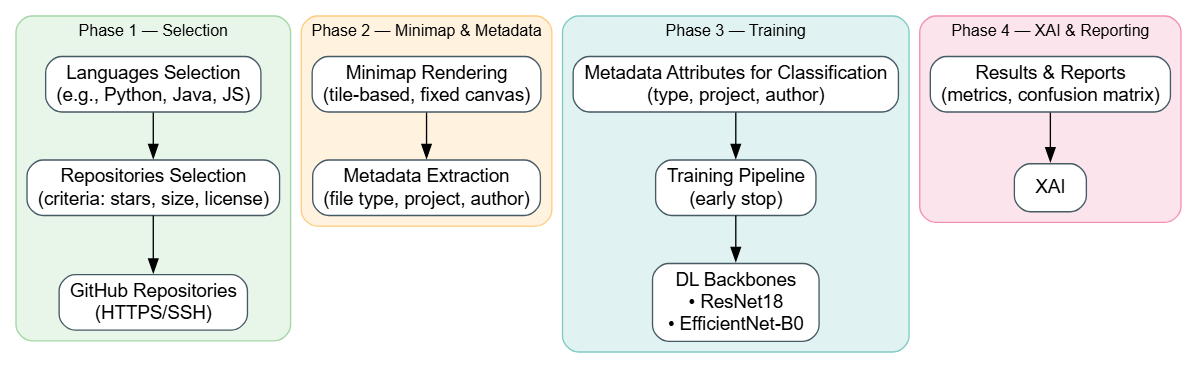
\includegraphics[width=0.95\textwidth]{figuras/workflow.png}
    \fautor
\end{figure}

The pipeline is intentionally modular. Minimap generation can be executed
without model training; anonymization can be strengthened or replaced; the same
catalog can support different objectives; and the trained models can be used
either in offline experiments or in IDE-integrated inference. This modularity is
important because the doctoral project combines empirical research, dataset
construction, explainability, and tool support.

\section{Repository Selection and File Discovery}

The repository-selection strategy depends on the research objective. For the
large-scale study, repositories were selected to cover multiple programming
languages and project conventions. The resulting corpus contains 100 open-source
projects across 10 languages \cite{gebara2025ciarp}. For future quality-related
studies, the selection must be refined to include repositories with known
quality indicators, code-smell labels, architectural roles, or defect history.

File discovery starts with recursive traversal of each repository. The traversal
records the relative path, file extension, size, and repository identifier. It
also applies exclusion rules to avoid files that would distort the dataset or
introduce redundant information. Typical exclusions include version-control
metadata, dependency folders, build outputs, binaries, vendored libraries, and
generated distribution folders such as \texttt{node\_modules}, \texttt{dist},
\texttt{build}, and \texttt{target}.

The filtering strategy must balance coverage and noise. If filtering is too
strict, the dataset may lose relevant software artifacts such as configuration
files, templates, and markup. If filtering is too permissive, the dataset may be
dominated by generated files, vendored code, or non-source artifacts. Because
minimaps can represent heterogeneous file types, the project does not restrict
the corpus to one programming language. Instead, file types are included when
they are meaningful for software analysis and when their role can be documented
in the catalog.

\section{Minimap Generation}

A source code minimap is generated by mapping the characters of a source file to
pixel intensities. The simplest form treats each character position as a visual
unit and each line as a row. The resulting image preserves aspects such as line
length, indentation, blank lines, punctuation density, and repeated structures.
Figure~\ref{fig:minimap-generation} illustrates the transformation from source
code to minimap.

\begin{figure}[ht]
    \centering
    \caption{Transformation of source code into a minimap representation.}
    \label{fig:minimap-generation}
    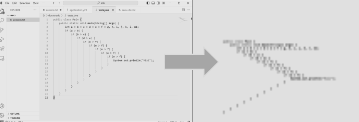
\includegraphics[width=0.88\textwidth]{figuras/minimap-generation.png}
    \fautor
\end{figure}

Two rendering strategies are considered:

\begin{description}
    \item[Variable-size minimaps.] The image width follows the length of the
    longest line, and the height follows the number of lines in the file. This
    representation preserves more information from the original artifact, but it
    produces images of different dimensions.

    \item[Fixed-size minimaps.] Each file is rendered or resized to a standard
    dimension, such as 128 by 128 pixels. This representation simplifies deep
    learning pipelines because all inputs share the same shape.
\end{description}

Figure~\ref{fig:fixed-variable} contrasts fixed-size and variable-size minimaps.
The first study evaluated both alternatives with handcrafted texture
descriptors, while the large-scale study adopted fixed 128 by 128 minimaps for
compatibility with convolutional backbones \cite{gebara2025iwssip,gebara2025ciarp}.

\begin{figure}[ht]
    \centering
    \caption{Comparison between variable-size and fixed-size minimaps.}
    \label{fig:fixed-variable}
    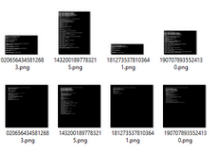
\includegraphics[width=0.82\textwidth]{figuras/fixed-variable-minimaps.png}
    \fautor
\end{figure}

Algorithm~\ref{alg:minimap-generation} summarizes the minimap generation
procedure in abstract form.

\begin{algorithm}[ht]
\caption{Source code minimap generation}
\label{alg:minimap-generation}
\begin{algorithmic}[1]
\Require Repository path $R$, file filters $F$, anonymization function $A$, target size $S$
\Ensure Minimap image set $M$ and metadata catalog $C$
\State $M \gets \emptyset$; $C \gets \emptyset$
\ForAll{file $f$ discovered recursively in $R$}
    \If{$f$ satisfies filters $F$}
        \State $content \gets$ read textual content from $f$
        \State $content' \gets A(content)$
        \State $image \gets$ render characters of $content'$ as pixel intensities
        \If{fixed-size mode is enabled}
            \State $image \gets$ resize or pad $image$ to target size $S$
        \EndIf
        \State $id \gets$ compute stable artifact identifier
        \State Add $(id, image)$ to $M$
        \State Add metadata for $f$ to $C$
    \EndIf
\EndFor
\State \Return $M, C$
\end{algorithmic}
\end{algorithm}

\section{Anonymization Strategy}

Anonymization is central to the project because it enables analysis of
industrial and proprietary codebases without exposing business-sensitive
information. A source file may embed strategic knowledge in identifiers
(\texttt{calculateMargin}, \texttt{profitRate}), in numeric constants
(\texttt{23.45}, \texttt{0.031}), or in comments describing business rules.
Sending such a file to an external analysis service---even in a research
context---can disclose intellectual property that organizations are not willing
to share. The minimap approach addresses this by suppressing the lexical layer
before the representation is transmitted or stored externally.

The initial anonymization strategy maps broad character classes to canonical
values. Letters and digits are replaced by representative values, while
whitespace and structural symbols are preserved. This suppresses all identifiers,
numeric literals, and string content while retaining visual signals such as
indentation, brackets, operators, separators, and line density.

Figure~\ref{fig:anonymization} shows an example of minimap generation before and
after anonymization.

\begin{figure}[ht]
    \centering
    \caption{Minimap rendering before and after anonymization.}
    \label{fig:anonymization}
    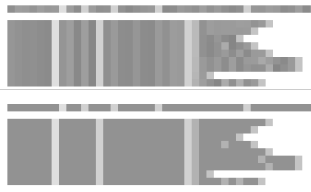
\includegraphics[width=0.82\textwidth]{figuras/anonymization.png}
    \fautor
\end{figure}

Table~\ref{tab:anonymization} summarizes the character-to-pixel mapping strategy
adopted in the current implementation. Each character in the source file is
mapped to a grayscale intensity value before the minimap image is generated.
Pixel values range from 0 to 255.

\begin{table}[ht]
\centering
\caption{Character-to-pixel mapping strategy used in the current implementation.}
\label{tab:anonymization}
\begin{tabular}{p{0.26\textwidth}p{0.12\textwidth}p{0.12\textwidth}p{0.33\textwidth}}
\toprule
\textbf{Character class} & \textbf{ASCII range} & \textbf{Pixel value} & \textbf{Information effect} \\
\midrule
Control characters and whitespace & below 32 & 0 & Preserves blank-line and indentation structure. \\
Digits & 48--57 & 53 & Suppresses numeric literals; marks numeric regions. \\
Uppercase letters & 65--90 & 77 & Suppresses identifiers; marks uppercase density. \\
Lowercase letters & 97--122 & 109 & Suppresses identifiers; marks lowercase density. \\
All other printable characters (spaces, punctuation, symbols, operators) & remaining & raw ASCII value & Preserves structural delimiters, operators, and layout signals. \\
\bottomrule
\end{tabular}
\fautor
\end{table}

A preliminary comparison between anonymized and non-anonymized minimaps was
conducted during the development of the approach. The results showed that
predictive performance is largely preserved after anonymization, confirming
that the discriminative signals captured by the model reside in structural
features---indentation, operator density, punctuation layout---rather than in
identifier names or literal values. This finding strengthens the argument that
anonymization can be applied without substantially sacrificing utility, and
that the model genuinely operates on structure rather than on lexical content.

This anonymization strategy is deliberately limited in its privacy claims. It
removes the lexical layer that carries direct business information, but it does
not guarantee unrecoverability of all organizational signals. A distinctive
architectural pattern or a very unusual indentation idiom could remain
recognizable. Stronger transformations---such as removing comments, normalizing
indentation, or masking punctuation density---can be evaluated in future work
as part of the suppression trade-off analysis (Activity A2).

\section{Catalog Construction}

Each generated minimap must be accompanied by a catalog. Without a catalog, the
image dataset becomes difficult to audit, reproduce, split, or extend. The
catalog records the metadata needed for supervised learning and later analysis.
Table~\ref{tab:catalog-fields} lists the core fields.

\begin{table}[ht]
\centering
\caption{Core fields of the minimap catalog.}
\label{tab:catalog-fields}
\begin{tabular}{p{0.25\textwidth}p{0.58\textwidth}}
\toprule
\textbf{Field} & \textbf{Purpose} \\
\midrule
Artifact identifier & Stable identifier for the generated minimap. \\
Repository identifier & Project-level label and provenance. \\
Hashed relative path & Path reference without exposing the original path. \\
File extension or inferred type & Basis for Type classification and filtering. \\
Programming language & Language-level grouping and analysis. \\
Author or committer label & Basis for the Author objective when ethically appropriate. \\
Image path & Location of the generated minimap file. \\
Split assignment & Train, validation, or test partition. \\
Anonymization mode & Transformation applied before rendering. \\
\bottomrule
\end{tabular}
\fautor
\end{table}

The catalog enables traceability between the original repository, the generated
image, and the learning objective. It also supports later filtering. For
example, a researcher may create a balanced Type subset, exclude bot authors,
select only Java projects, or design repository-disjoint splits. This makes the
catalog as important as the image files themselves.

\section{Dataset Splitting and Leakage Control}

Dataset splitting is one of the most important methodological decisions in this
project. A random file-level split is simple, but it may introduce leakage. If
near-duplicate files, generated templates, or files from the same repository
appear in both training and test sets, performance may be inflated. This risk is
especially relevant for Project and Author objectives because repository
conventions and contributor patterns can be repeated across many files.

The methodology therefore distinguishes three split strategies:

\begin{description}
    \item[File-stratified split.] Files are split while preserving class
    proportions. This strategy is useful for initial model development, but it
    is vulnerable to repository-level leakage.

    \item[Repository-aware split.] Repositories or repository groups are used to
    control which artifacts can appear in each partition. This strategy is
    stronger when the goal is to evaluate cross-project generalization.

    \item[Time-aware split.] Files or commits are split according to time. This
    strategy is useful when the goal is to simulate future prediction from past
    data, but it requires reliable historical metadata.
\end{description}

The appropriate split depends on the research question. For Type classification,
a stratified split may be acceptable when the question is whether minimaps encode
file-role signals within a corpus. For generalization claims, repository-aware
or time-aware splits are stronger. For Author analysis, additional care is
required because aliases, bots, and organizational accounts may distort the
meaning of labels.

Leakage control also requires preprocessing. The dataset-generation pipeline
should compute content hashes, identify exact duplicates, and flag near
duplicates when possible. Generated files should be detected or at least marked
in the catalog. Templates and boilerplate should be analyzed with ablation
experiments because they may dominate predictions.

\section{Prediction Objectives}

The large-scale study uses three supervised objectives: Type, Project, and
Author \cite{gebara2025ciarp}. These objectives are not equally sensitive and
must be interpreted differently.

\begin{description}
    \item[Type.] The model predicts the file-role or file-type class. This
    objective evaluates whether minimaps preserve artifact-level structural
    differences. It is the most directly relevant objective for future code
    quality and comprehension tasks.

    \item[Project.] The model predicts the repository from which a minimap was
    extracted. This objective evaluates whether minimaps capture repository
    conventions, templates, boilerplate, and project-specific organization.

    \item[Author.] The model predicts the author or committer label associated
    with the file. This objective is treated as a research proxy for stylistic
    and contribution-pattern signals. It must be handled carefully because
    author prediction can raise ethical and attribution concerns.
\end{description}

These objectives provide complementary evidence. Type asks whether minimaps can
recognize artifact roles. Project asks whether minimaps encode repository
identity. Author asks whether anonymized visual structure still contains
style-related cues. Together, they test whether minimaps preserve information at
different levels of granularity.

\section{Extension Toward Quality-Related Tasks}

Type, Project, and Author objectives are useful for validating the
representation, but the long-term thesis should also investigate tasks closer to
software quality. A minimap may not directly encode whether a method is correct,
but it can provide signals about structure, density, repetition, generated
regions, and deviations from project conventions. These signals can support
quality-related analysis when combined with appropriate labels.

Three task families are planned:

\begin{description}
    \item[Artifact-role consistency.] The model predicts whether a file visually
    conforms to its expected role. For example, a file labeled as a test may be
    compared with other tests in the same project.

    \item[Quality proxy classification.] The model predicts labels derived from
    existing tools, such as smell presence, complexity thresholds, or static-rule
    violations. These labels are noisy but useful for exploratory analysis.

    \item[Architectural-deviation detection.] The model identifies files whose
    visual signatures differ substantially from project-specific conventions for
    the same role.
\end{description}

These tasks require caution. A visual anomaly is not necessarily a defect. A
file may look unusual because it implements a legitimate special case. The
methodology should therefore frame minimap-based quality analysis as
prioritization or decision support, not automated judgment. The output should
help reviewers decide where to look, not replace the review.

\section{Learning Pipelines}

The methodology includes two main learning pipelines. The first uses
handcrafted texture descriptors. Minimap images are converted into Local Binary
Pattern histograms, and classifiers such as K-Nearest Neighbors, Random Forest,
and Support Vector Machines are trained over the resulting feature vectors
\cite{gebara2025iwssip}. This pipeline is useful as a baseline because it is
simple, efficient, and connected to previous texture-analysis literature.

The second pipeline uses deep learning. Fixed-size minimaps are passed directly
to convolutional backbones such as ResNet-18 and EfficientNet-B0, with both
from-scratch and pretrained variants considered \cite{he2016resnet,tan2019efficientnet,gebara2025ciarp}.
The model is trained end-to-end with task-specific output heads. This pipeline
can learn visual features directly from minimap images and may capture patterns
that handcrafted descriptors miss.

The comparison between these pipelines helps answer RQ2. If handcrafted
descriptors already perform well, then minimaps contain strong texture-level
signals. If deep models significantly improve results, then learned
representations capture additional structure. If both struggle on certain
classes, then the representation or labels may need refinement.

\section{Evaluation Metrics}

Evaluation must account for multi-class classification and severe class
imbalance. Accuracy is intuitive, but it can overstate performance when large
classes dominate. Macro-F1 gives equal weight to each class and is therefore
important for minority-class behavior. Weighted-F1 accounts for class support and
reflects performance under the observed distribution. ROC-AUC, reported in macro
and micro forms, helps assess separability across classes.

Table~\ref{tab:metrics} summarizes the metrics used in the project.

\begin{table}[ht]
\centering
\caption{Evaluation metrics used in minimap classification.}
\label{tab:metrics}
\begin{tabular}{p{0.20\textwidth}p{0.33\textwidth}p{0.34\textwidth}}
\toprule
\textbf{Metric} & \textbf{What it measures} & \textbf{Why it is useful here} \\
\midrule
Accuracy & Overall proportion of correct predictions. & Provides a direct global measure. \\
Macro-F1 & Mean F1 across classes with equal class weight. & Highlights minority-class performance. \\
Weighted-F1 & F1 averaged by class support. & Reflects performance under the dataset distribution. \\
Macro ROC-AUC & Class-balanced separability. & Useful under multi-class imbalance. \\
Micro ROC-AUC & Global separability across decisions. & Captures overall ranking behavior. \\
Confusion matrix & Distribution of correct and incorrect predictions. & Reveals which classes are confused. \\
\bottomrule
\end{tabular}
\fautor
\end{table}

Class imbalance is not only a metric problem. It can influence training,
generalization, and interpretation. Prior studies on imbalanced data
\cite{he2009imbalance,japkowicz2002,ortigosa2017} motivate the use of
class-aware metrics and future experiments with reweighting, focal loss,
balanced sampling, and calibration analysis.

\section{Qualitative Analysis}

Quantitative metrics are necessary but insufficient. A high score does not
explain what the model learned, whether the representation is meaningful, or how
the result should be used. For this reason, the methodology includes qualitative
analysis at three levels.

First, sample inspection is used during dataset construction. For each class,
the researcher should inspect randomly selected minimaps, representative
examples, and outliers. This helps identify mislabeled files, generated
artifacts, corrupt images, and classes that are visually heterogeneous.

Second, confusion analysis is used after model evaluation. When two classes are
frequently confused, the researcher should inspect their minimaps and labels.
Some confusion may be expected, such as between visually similar Java roles.
Other confusion may indicate problems in preprocessing or label definitions.

Third, explanation analysis is used to inspect attribution maps. If a model
focuses on file borders, compression artifacts, or dataset-specific noise, the
result is less trustworthy. If it focuses on indentation bands, delimiter
regions, or structural blocks, the result is more consistent with the research
hypothesis.

These qualitative procedures make the methodology more robust. They also help
transform model outputs into research insight.

\section{Explainability Protocol}

The explainability protocol uses Integrated Gradients to attribute predictions
to input pixels \cite{integratedgradients2017}. For each task, a trained model
receives a minimap image, and the attribution method estimates which regions
contribute most to the predicted class. The attribution map is normalized and
overlaid on the input image to support qualitative analysis.

The protocol is used to answer RQ3. In particular, it asks whether Type
classification relies on structural regions, whether Project classification uses
boilerplate or repository conventions, and whether Author classification depends
on diffuse style-related patterns. These interpretations help identify both
strengths and risks. A model that relies heavily on generated headers, for
example, may perform well but generalize poorly to repositories without that
boilerplate.

\section{Reproducibility and Artifact Strategy}

Reproducibility is a central requirement of the proposed methodology. The
project therefore separates artifacts into five categories:

\begin{enumerate}
    \item minimap generation scripts;
    \item anonymization procedures;
    \item image datasets and metadata catalogs;
    \item training and evaluation configurations;
    \item IDE plugins and backend services.
\end{enumerate}

The public code organization for the tool ecosystem is
\url{https://github.com/minimap-project}. The dataset used in the large-scale
study is available through Zenodo, and the training infrastructure is maintained
in public repositories. These artifacts support independent inspection and
future extensions, but they also require versioning discipline. Each experiment
should record the repository snapshot, dataset version, random seed, model
configuration, preprocessing mode, and evaluation split.

The methodology therefore treats reproducibility not as an afterthought but as
part of the research object. A minimap-based approach is only useful if other
researchers can regenerate representations, audit labels, compare models, and
extend the corpus to new tasks.

\section{Implementation Considerations}

The implementation of the methodology must address several engineering details.
Text files may use different encodings, line endings, and character sets.
Repositories may contain very large files, binary files with misleading
extensions, or generated artifacts. Rendering must be deterministic so that the
same file and anonymization mode produce the same minimap. Catalog generation
must also be deterministic so that image identifiers can be reproduced.

Performance is another concern. A large repository may contain thousands of
files, and a corpus with 100 repositories can generate hundreds of thousands of
images. The pipeline should support incremental generation, caching, and
parallel processing when possible. It should also log failures explicitly
instead of silently skipping problematic files.

For IDE integration, implementation constraints are different. A plugin must
generate a minimap quickly enough that the developer does not experience the
operation as disruptive. It must avoid sending raw source code when the
anonymized minimap is sufficient. It must handle unsaved buffers, temporary
files, and different editor encodings. These practical details are part of the
method because they determine whether minimap analysis can move from offline
experiments to developer workflows.

Finally, versioning is essential. A model trained with one anonymization
function and rendering procedure may not be compatible with minimaps generated
by another version of the tool. Therefore, each minimap and model should record
the rendering version, anonymization mode, target size, model version, and label
mapping. Without this metadata, predictions become difficult to audit.


\chapter{Preliminary Studies and Results}
\label{chapter:preliminary-results}
This chapter reports the empirical work already completed. Three studies are
described in sequence. The first two are ordered from the most controlled to the
most demanding setting: a small, balanced experiment with handcrafted texture
descriptors, and a large-scale experiment with deep convolutional models over
hundreds of thousands of minimaps. The third isolates a single question that the
proposal depends on, whether anonymization costs predictive performance, and
answers it with a paired design and an explicit statistical statement. The
chapter then consolidates what the studies jointly support, maps that evidence
back to the research questions, and is explicit about the limitations that
prevent the current results from being read as final. The research plan of
Chapter~\ref{chapter:research-plan} is built to resolve them.

\section{Role of Preliminary Studies}

This chapter consolidates the empirical evidence already produced during the
doctoral research. The goal is not to present the final thesis results, but to
show that the proposed direction is viable and that the remaining work is built
on concrete artifacts. Two studies are central. The first evaluates source code
minimaps with Local Binary Patterns and traditional machine learning
\cite{gebara2025iwssip}. The second scales the approach to hundreds of thousands
of minimaps and evaluates deep learning models with explainability
\cite{gebara2025ciarp}. A third study isolates the anonymization question with a
paired design.

Together, these studies support four claims. First, source code minimaps encode
discriminative information about software artifacts. Second, both handcrafted
texture descriptors and learned visual representations can exploit this
information. Third, explainability methods can reveal which visual regions
models use when making predictions. Fourth, suppressing lexical content does not
cost predictive performance in the setting where this has been measured, even
though it removes more than half of the information carried by each pixel.

\section{Study 1: Feature Detection with Texture Descriptors}

The first study introduced source code minimaps as visual signatures for
software feature detection \cite{gebara2025iwssip}. The methodology generated
minimap images from source files, applied anonymization, extracted Local Binary
Pattern histograms, and trained traditional classifiers. The evaluated models
included K-Nearest Neighbors, Random Forest, and Support Vector Machines.

The study was motivated by the observation that software artifacts often have
visual texture. Some classes contain repeated fields and annotations, some test
files contain repeated assertions and setup methods, some front-end files contain
dense markup, and some configuration files contain short nested structures.
Instead of manually defining rules for each stereotype, the study asked whether
these visual patterns could be learned from minimap images.

Figure~\ref{fig:lbp} illustrates the Local Binary Pattern operator used as the
texture descriptor.

\begin{figure}[ht]
    \centering
    \caption{Local Binary Pattern operator used for texture extraction.}
    \label{fig:lbp}
    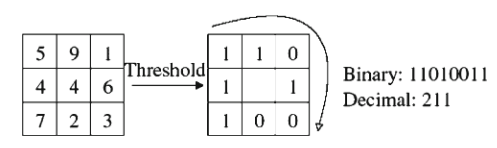
\includegraphics[width=0.70\textwidth]{figuras/lbp.png}
    \fadaptada{martins2013database}
\end{figure}

The operator works as follows \cite{ojala2002lbp}. Each pixel of the image is
taken in turn as the center of a neighborhood, and its intensity is used as a
local threshold. Every neighbor is compared with the center and replaced by a
single bit: one if the neighbor is greater than or equal to the center, zero
otherwise. In the example of Figure~\ref{fig:lbp}, the center value 4 converts
the surrounding intensities into the bits shown in the middle grid. Reading
these bits in a fixed circular order produces a binary word, here 11010011,
whose decimal value 211 becomes the code assigned to that pixel. Two parameters
control the operator: the number of sampled neighbors and the radius of the
circle on which they lie, which together determine the spatial scale of the
pattern being described.

Applying this procedure to every pixel yields a code image, and the descriptor
of the minimap is the histogram of those codes. Taking the histogram is the step
that makes the representation useful: it discards where each pattern occurred
and retains only how often each local configuration appears, so two files with the same
layout conventions produce similar descriptors even when their content differs.
The study used eight sampling points on a radius of two pixels and the
non-rotation-invariant uniform variant of the operator, which keeps every
uniform pattern, i.e., every code with at most two bit transitions in the
circular word, as an individual bin and collapses the remaining codes into a
single bin. This yields a descriptor of 59 bins per minimap, normalized to sum
to one so that images of different sizes remain comparable.

Two properties explain why this operator is a reasonable first choice for
minimaps. It is invariant to monotonic changes in overall intensity, because
only comparisons between neighbors matter, and it responds to exactly the kind
of structure a minimap encodes: indentation steps, line endings, and dense
punctuation regions all appear as recurring local intensity transitions rather
than as objects with semantic boundaries.

The study generated two dataset variants. The first used variable-size minimaps,
where image dimensions reflected source file dimensions. The second used
fixed-size minimaps, especially 128 by 128 pixels, to support later comparison
with neural image models. This distinction is important because variable-size
minimaps preserve more original layout information, while fixed-size minimaps
simplify modeling.

\subsection{Dataset and Classes}

The initial dataset was generated from two large private software projects, made
available under a confidentiality agreement: an enterprise resource planning
system from a company in the industrial sector, and a system developed by the
Brazilian federal government. Their size and heterogeneity made them a realistic
basis for the study, and they could only be used because anonymization removed
the lexical layer. Processing them produced 42,820 minimap images, organized into 28
classes representing file types and Java-related stereotypes, including Java
entities, repositories, services, unit tests, JavaScript files, JSON files, SVG
files, XML files, properties files, shell scripts, and SQL files. The complete
raw class distribution was imbalanced, with some classes containing only a few
instances and others containing thousands.

One implementation detail of the generation step affects the descriptor. An
eight-pixel dead zone was added around every image in both dataset variants, so
that the LBP operator can be evaluated on pixels near the original borders
without discarding them.

For the first controlled evaluation, the study kept only classes with more than
1,000 examples and drew exactly 1,000 random samples from each, which yields a
balanced setting. This produced seven classes: JSON, SVG, JavaScript, JSP, and
the Java stereotypes Entity, UnitTest, and ServiceImplementation. The design
provided a controlled scenario in which to test whether the representation
itself contained useful visual signals.

The published article does not report the partitioning scheme, so the protocol
described here was recovered from the accompanying artifact repository and
should be read as a reconstruction. Classes are capped as described above and
the resulting descriptor matrix is split once into 80\% training and 20\% test
partitions under a fixed random seed. Hyperparameters for each classifier are
selected by grid search with five-fold cross-validation over the training
partition only, and the test partition is used exclusively for the reported
figures. Two limitations of this protocol should be stated explicitly. The split
is not stratified by class label, so balance in the test partition follows from
the sampling cap rather than from the splitting procedure itself; and because a
single split is used, the reported values carry no variance estimate. Recording
the protocol explicitly and repeating the evaluation over multiple seeds is part
of the planned work described in Chapter~\ref{chapter:research-plan}.

Figure~\ref{fig:lbp-histograms} presents average LBP histograms for six
representative classes, computed over 1{,}000 minimaps per class. The figure is
split into two panels because the descriptor has a strongly skewed shape. Two
codes dominate every class: the code produced by a flat neighborhood and the
catch-all bin for non-uniform patterns. Together they account for between 91\%
and 99\% of the mass, which is expected, since a minimap is mostly empty
background. The upper panel shows the complete descriptor on a logarithmic
scale so that this dominance is visible; the lower panel restricts the view to
the remaining codes on a linear scale, where the classes actually separate.

\begin{figure}[ht]
    \centering
    \caption{Average LBP histograms for six minimap classes. Upper panel:
    complete descriptor, logarithmic scale. Lower panel: codes 0--56, linear
    scale.}
    \label{fig:lbp-histograms}
    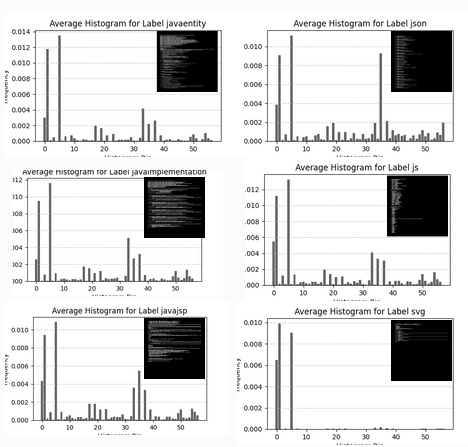
\includegraphics[width=0.92\textwidth]{figuras/lbp-histograms.png}
    \fautor
\end{figure}

Read this way, the figure carries a more precise message than a claim of visual
similarity. The discriminative structure occupies a small fraction of the
descriptor, from 0.4\% of the mass for SVG files to 7.5\% for JSP pages, and it
is concentrated in a few codes that correspond to horizontal and vertical
intensity transitions, i.e., to line endings and indentation steps. The classes
separate mostly by how much of that structure they contain and in which
proportion. SVG files are an instructive case: their minimaps are almost
entirely flat, so their descriptor is nearly degenerate, yet this very emptiness
makes them trivially separable from every other class. Java entity and Java
implementation files, in contrast, produce nearly superposed profiles, which
anticipates the confusion observed between them in the results below.

\subsection{Results}

Table~\ref{tab:study1-results} summarizes the main performance results reported
for the three traditional classifiers. The published study reports a single
figure of merit, overall accuracy on the test partition, and the table therefore
reports that quantity alone.\footnote{Earlier versions of this table presented
the same value under three separate headings for precision, recall, and
F1-score. That presentation was misleading: no per-class or averaged
precision-recall figures were computed for this experiment. Producing them, from
the per-class classification reports that the pipeline already generates, is
part of the consolidation work described in
Chapter~\ref{chapter:research-plan}.} The values should be interpreted as
preliminary evidence, both because the dataset was limited when compared with
the later large-scale corpus and because accuracy alone says nothing about how
the errors are distributed across classes.

\begin{table}[ht]
\centering
\caption{Summary of preliminary results with LBP features.}
\label{tab:study1-results}
\begin{tabular}{p{0.34\textwidth}c}
\toprule
\textbf{Classifier and dataset} & \textbf{Accuracy} \\
\midrule
KNN, variable-size minimaps & 0.79 \\
KNN, fixed-size minimaps & 0.78 \\
Random Forest, variable-size minimaps & 0.93 \\
Random Forest, fixed-size minimaps & 0.93 \\
SVM, variable-size minimaps & 0.89 \\
SVM, fixed-size minimaps & 0.88 \\
\bottomrule
\end{tabular}
\fautor
\end{table}

Random Forest achieved the best overall results, reaching approximately 93\%
accuracy in both fixed-size and variable-size settings. This result is
important because it indicates that minimap texture contains discriminative
signals even before using deep learning. SVM also performed strongly, while KNN
was less effective, suggesting that the feature space benefits from models that
can learn more complex decision boundaries or ensemble combinations. Across all
three classifiers the variable-size minimaps are equal or marginally superior to
the fixed-size ones, by at most one percentage point, which is consistent with
the fact that resizing to 128 by 128 pixels discards layout information. The
margin is small enough that fixed-size minimaps remain the sensible choice for
the convolutional experiments that follow, where a uniform input size is
required.

Figure~\ref{fig:confusion-rf} shows the confusion matrices for Random Forest in
the fixed-size and variable-size settings. The matrices indicate strong
performance for visually distinctive classes such as JSON and SVG, while some
Java-related classes exhibit more confusion because they share structural
similarities.

\begin{figure}[ht]
    \centering
    \caption{Random Forest confusion matrices for fixed-size and variable-size minimaps.}
    \label{fig:confusion-rf}
    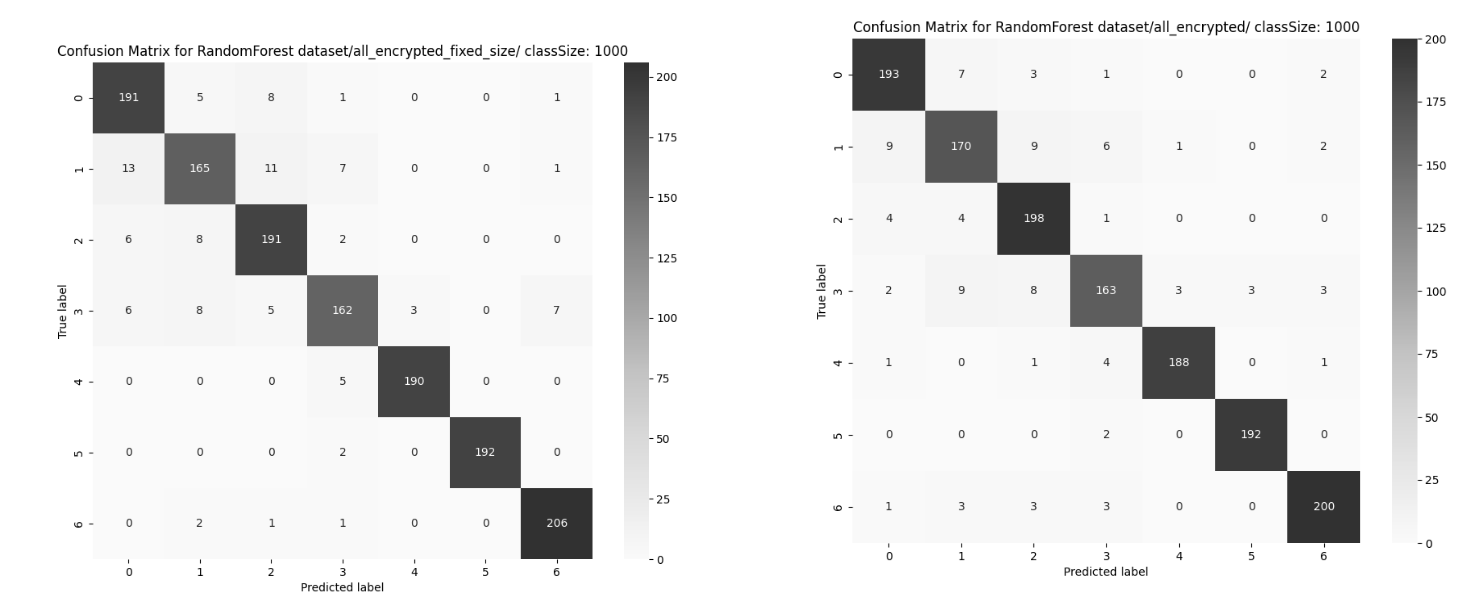
\includegraphics[width=0.92\textwidth]{figuras/confusion-rf.png}
    \fautor
\end{figure}

\subsection{Lessons from Study 1}

The first study produced four lessons that guide the rest of the doctorate.
First, source code minimaps can support classification without relying on
language-specific parsers. Second, anonymization did not prevent the models from
learning useful visual patterns in the evaluated setting. Third, fixed-size
minimaps remained competitive with variable-size minimaps, making them suitable
for convolutional models. Fourth, class similarity matters: files with similar
roles and layouts may be difficult to separate with texture descriptors alone.

These lessons motivated the second study. If minimaps work with handcrafted
features in a limited setting, the next question is whether they scale to more
projects, languages, classes, and learning objectives.

\section{Study 2: Large-Scale Deep Learning}
\label{sec:study2}

The second study expanded the evaluation to a large-scale corpus of source code
minimaps \cite{gebara2025ciarp}. The dataset contains 685,906 minimap images
extracted from 100 open-source projects across 10 programming languages. The
images are standardized to 128 by 128 pixels and accompanied by a file-level
catalog. The study evaluates three objectives: Type, Project, and Author.

The scale of the dataset changes the nature of the problem. Instead of asking
whether a few visually distinct classes can be separated, the study asks whether
minimaps preserve useful information across many repositories and heterogeneous
ecosystems. It also introduces severe class imbalance, especially because some
projects and file types are much more frequent than others.

Figure~\ref{fig:dist-type} presents the distribution of the top Type classes,
while Figures~\ref{fig:dist-project} and \ref{fig:dist-author} present the top
Project and Author classes.

\begin{figure}[ht]
    \centering
    \caption{Top Type classes in the large-scale minimap dataset.}
    \label{fig:dist-type}
    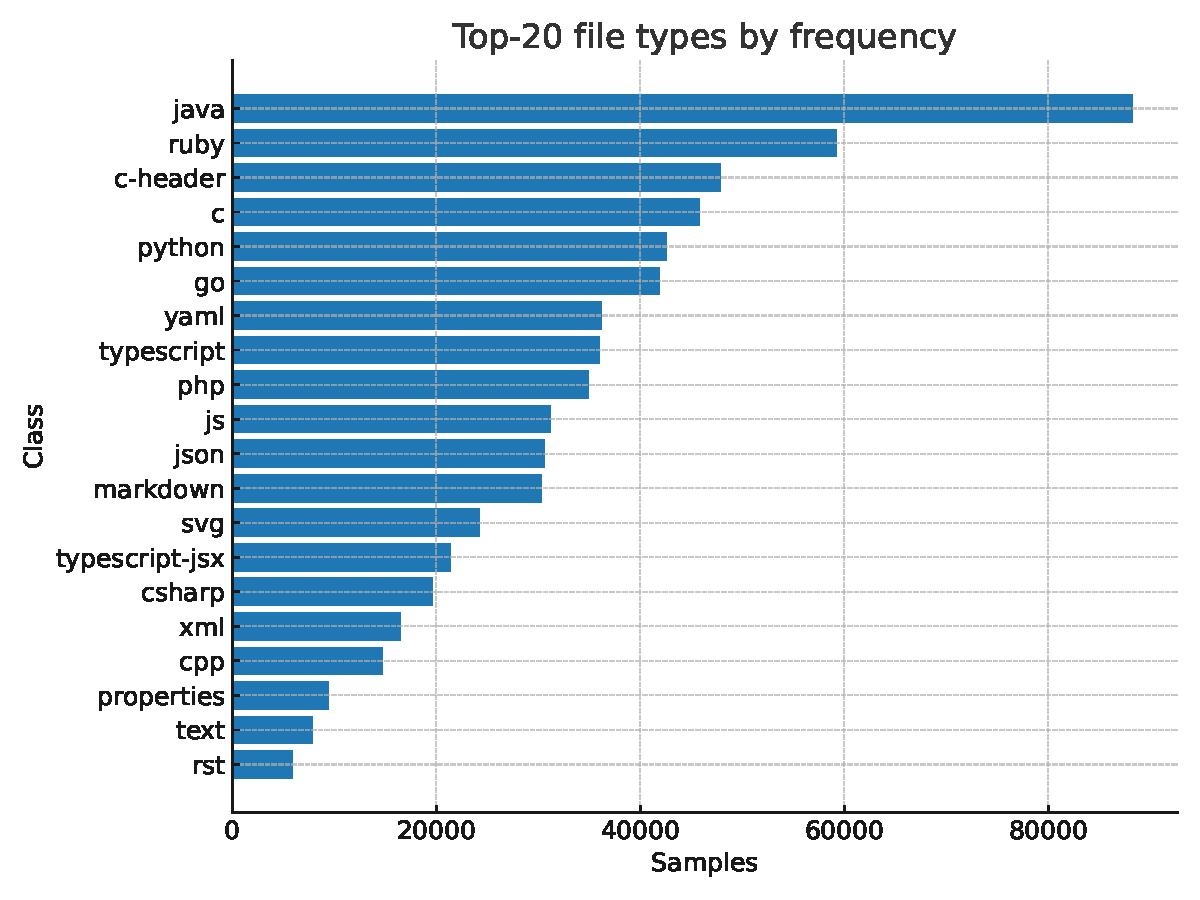
\includegraphics[width=0.82\textwidth]{figuras/dist-type-top20.pdf}
    \fautor
\end{figure}

\begin{figure}[ht]
    \centering
    \caption{Top Project classes in the large-scale minimap dataset.}
    \label{fig:dist-project}
    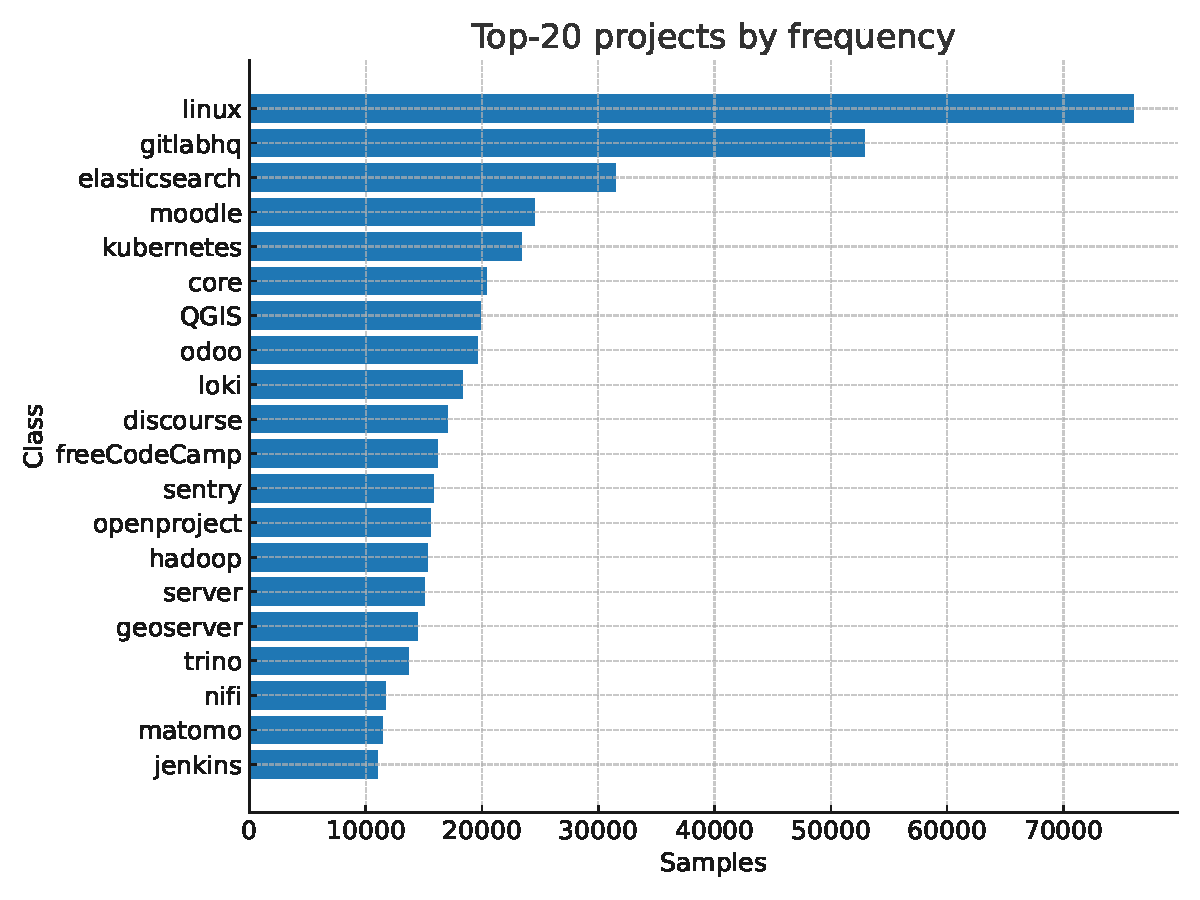
\includegraphics[width=0.82\textwidth]{figuras/dist-project-top20.pdf}
    \fautor
\end{figure}

\begin{figure}[ht]
    \centering
    \caption{Top Author classes in the large-scale minimap dataset.}
    \label{fig:dist-author}
    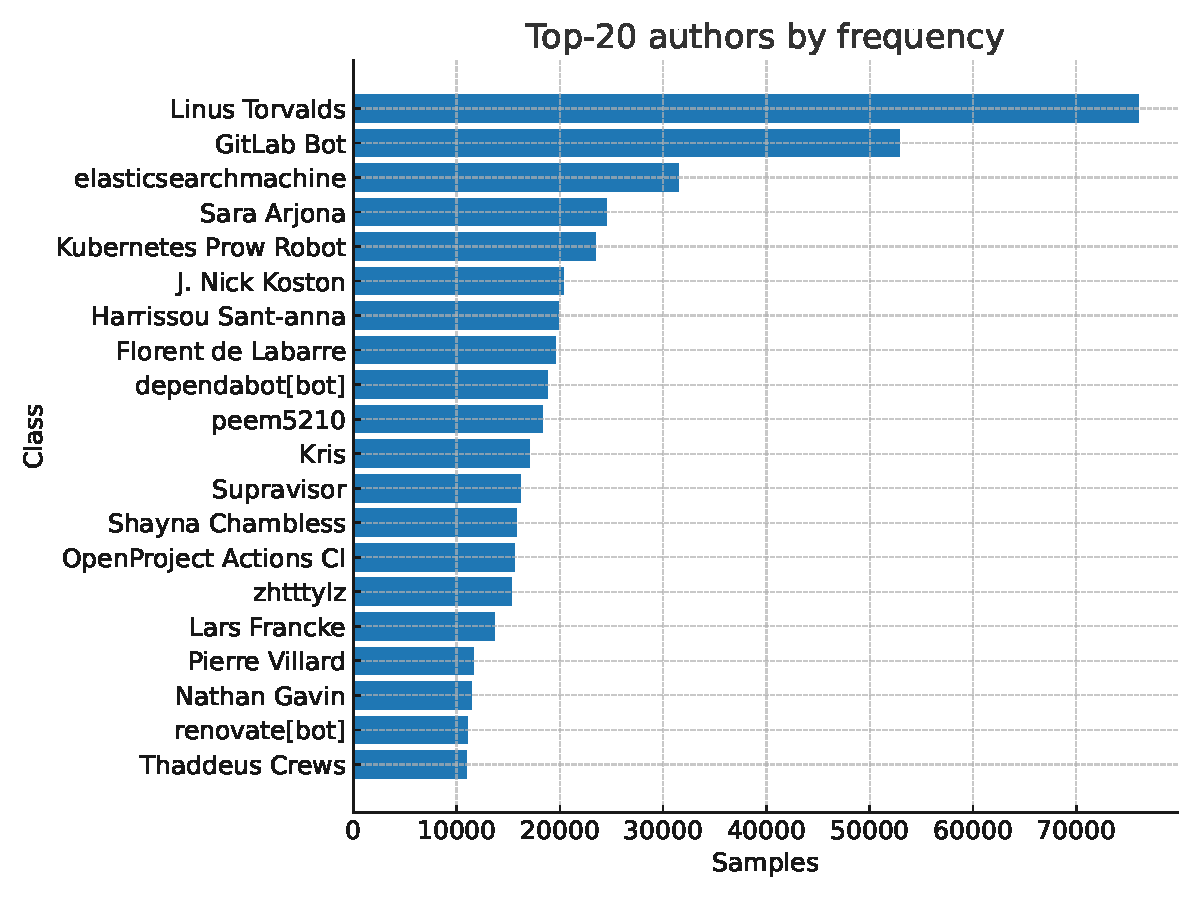
\includegraphics[width=0.82\textwidth]{figuras/dist-author-top20.pdf}
    \fautor
\end{figure}

\subsection{Dataset Summary}

Table~\ref{tab:study2-dataset} summarizes the main dataset statistics. The
numbers show that the corpus is large enough to train deep models, but also
imbalanced enough to require careful evaluation.

\begin{table}[ht]
\centering
\caption{Summary of the large-scale minimap dataset.}
\label{tab:study2-dataset}
\begin{tabular}{lr}
\toprule
\textbf{Property} & \textbf{Value} \\
\midrule
Number of minimap images & 685,906 \\
Number of open-source projects & 100 \\
Number of programming languages & 10 \\
Type classes & 63 \\
Project classes & 99 \\
Author classes & 97 \\
Default image size & 128 by 128 pixels \\
Default color mode & Grayscale \\
\bottomrule
\end{tabular}
\fautor
\end{table}

The Type objective contains file-role categories such as programming-language
files, headers, configuration formats, markup, scripts, and other artifacts. The
Project objective reflects repository identity.\footnote{The corpus was
generated from 100 repositories, while the label catalog records 99 distinct
Project classes. Documenting the precise origin of this one-class difference is
part of the dataset-curation activity (A1) in
Chapter~\ref{chapter:research-plan}.} The Author objective reflects
last-committer or author labels as recorded by the dataset-generation process.
Because this objective may conflate humans, bots, and organizational accounts,
it is interpreted cautiously.

\subsection{Training Protocol}

The large-scale study evaluates convolutional backbones under a unified
protocol. Inputs are fixed-size 128 by 128 grayscale minimaps. Models are
trained with early stopping and evaluated using accuracy and ROC-AUC, with
macro-F1 and weighted-F1 used to interpret class imbalance. The evaluated
architectures are ResNet-18 and EfficientNet-B0, tested in two
configurations: trained from scratch on the minimap corpus, and initialized
from ImageNet pretrained weights followed by fine-tuning
\cite{he2016resnet,tan2019efficientnet}. Vision Transformer configurations
(ViT-B/16) were also exercised during early experimentation, but the
consolidated evaluation focused on the two convolutional backbones; a
systematic transformer comparison is deferred to the research plan.

Three details of the data protocol matter for interpreting the results. Before splitting, classes with
fewer than 100 samples were excluded and classes were capped at 5,000 samples,
which limits extreme imbalance but also means that the effective number of
classes seen by the models can be smaller than the catalog totals. The data
were then split at file level into 70\% training, 15\% validation, and 15\%
test partitions, stratified by class label and controlled by a fixed random
seed. The split is not repository-disjoint: files from the same project can
appear in different partitions. For the Project objective this is unavoidable,
since each project is itself a class, but for Type and Author it means the
reported results are within-corpus validation; repository-disjoint evaluation
is part of the planned work. No data augmentation was applied: images are
converted to tensors and normalized with mean and standard deviation of 0.5.

The rationale for transfer learning is pragmatic. Although source code minimaps
are structurally different from natural images, pretrained convolutional filters
may still provide useful low-level edge and texture detectors. Results indicate
that ImageNet pretraining provides consistent but modest benefits across the
three objectives, with EfficientNet-B0 pretrained reaching the strongest
reported validation accuracy in this study \cite{gebara2025ciarp}.

\subsection{Results}

Table~\ref{tab:study2-results} presents the main validation results emphasized
in the large-scale study. EfficientNet-B0 with ImageNet pretraining reached the
best reported validation accuracies among the evaluated configurations. The
ROC-AUC values are reported as lower bounds, following the original study, and
the accuracies refer to the validation partition; consolidating the held-out
test results is part of the evaluation work described below.

\begin{table}[ht]
\centering
\caption{Representative validation results from the large-scale minimap study
(EfficientNet-B0, ImageNet pretrained).}
\label{tab:study2-results}
\begin{tabular}{p{0.20\textwidth}ccc}
\toprule
\textbf{Objective} & \textbf{Accuracy} & \textbf{ROC-AUC macro} & \textbf{ROC-AUC micro} \\
\midrule
Type    & 0.9333 & $\geq$0.99 & $\geq$0.99 \\
Project & 0.8604 & $\geq$0.99 & $\geq$0.99 \\
Author  & 0.8705 & $\geq$0.99 & $\geq$0.99 \\
\bottomrule
\end{tabular}
\fautor
\end{table}

The Type objective achieved the highest validation accuracy, which is
consistent with the research hypothesis: file roles often produce visually
distinctive structures that remain separable after character anonymization.
Project and Author classification are harder multi-class problems, with 99 and
97 labels respectively, yet the model still reached substantial accuracy,
suggesting that repository conventions and contributor style patterns are
partially encoded in the visual layout of source files even after lexical
content is suppressed.

The contrast between near-perfect ROC-AUC and accuracies of 86--87\% needs
explanation. With roughly one hundred classes evaluated
one-vs-rest, each per-class ROC curve is dominated by easy negatives: a model
can rank most negatives below the positives, and thus reach very high AUC,
while still confusing similar classes at decision time. Accuracy, in contrast,
requires the correct class to win among all labels. High AUC therefore signals
good per-class separability, not reliable final decisions. These values must
also be read together with imbalance-aware metrics, since large head classes
can dominate global accuracy while minority classes remain poorly classified.
The training pipeline already produces per-class classification reports and
confusion matrices for each objective; these outputs exist but have not yet
been consolidated into the tables above. Reporting macro-F1, per-class recall,
and held-out test results alongside the validation accuracies is a priority
for the next revision of these results, and improving minority-class behavior
remains one of the central open tasks.

\subsection{Explainability Findings}

The large-scale study uses Integrated Gradients \cite{integratedgradients2017}
to interpret model predictions. The method assigns to each input pixel the
integral of the model gradient along a straight path from a reference baseline
to the actual image, which distributes the difference in model output between
the two endpoints across the input pixels.

Three properties motivated this choice over the alternatives. First, the method
is defined by axioms rather than by architecture: it satisfies sensitivity,
meaning a pixel that changes the prediction receives non-zero attribution, and
implementation invariance, meaning functionally equivalent networks receive
identical attributions. Second, and decisively for this application, it produces
attributions at pixel resolution. Class activation methods such as Grad-CAM
\cite{selvaraju2017gradcam} operate on the last convolutional feature map, which
for a 128 by 128 input is reduced to a grid of a few cells; the visual evidence
of interest here, i.e., indentation steps, line endings, and delimiter columns,
is finer than that grid and would be blurred away. Third, the method is
gradient-based and therefore architecture-agnostic, which keeps the same
protocol usable when the evaluation is extended to transformer backbones, unlike
Grad-CAM, which presupposes a convolutional feature map. Perturbation-based
alternatives such as LIME and SHAP were not adopted because they require many
forward passes per explanation, which is impractical at the scale of this
corpus, and because their surrogate sampling is poorly defined for images whose
information is carried by thin, spatially structured strokes.

The protocol is the following. Attributions are computed with the Captum
implementation using 32 integration steps and a zero-valued baseline in the
normalized input space; since inputs are normalized with mean and standard
deviation of 0.5, this baseline corresponds to a uniform mid-gray image rather
than a black one. Attribution is always taken with respect to the class
predicted by the model, not the ground-truth label, so that the maps explain the
decision actually made. For each objective, eight validation images per class
are drawn under a fixed seed; the per-pixel attributions are reduced by absolute
value, summed across channels, min-max normalized per image, and then averaged
within each class and across all classes to yield the summaries reported here.
Two limitations follow directly from this design and should be kept in mind when
reading the maps: eight images per class is a small sample for a visual
argument, and the choice of baseline is known to influence attribution
magnitudes, so a baseline sensitivity check remains to be done.

Figure~\ref{fig:xai} presents attribution maps for the three objectives. The
figure suggests that models rely on different visual evidence depending on the
task.

\begin{figure}[ht]
    \centering
    \caption{Integrated Gradients attribution maps for minimap classification objectives.}
    \label{fig:xai}
    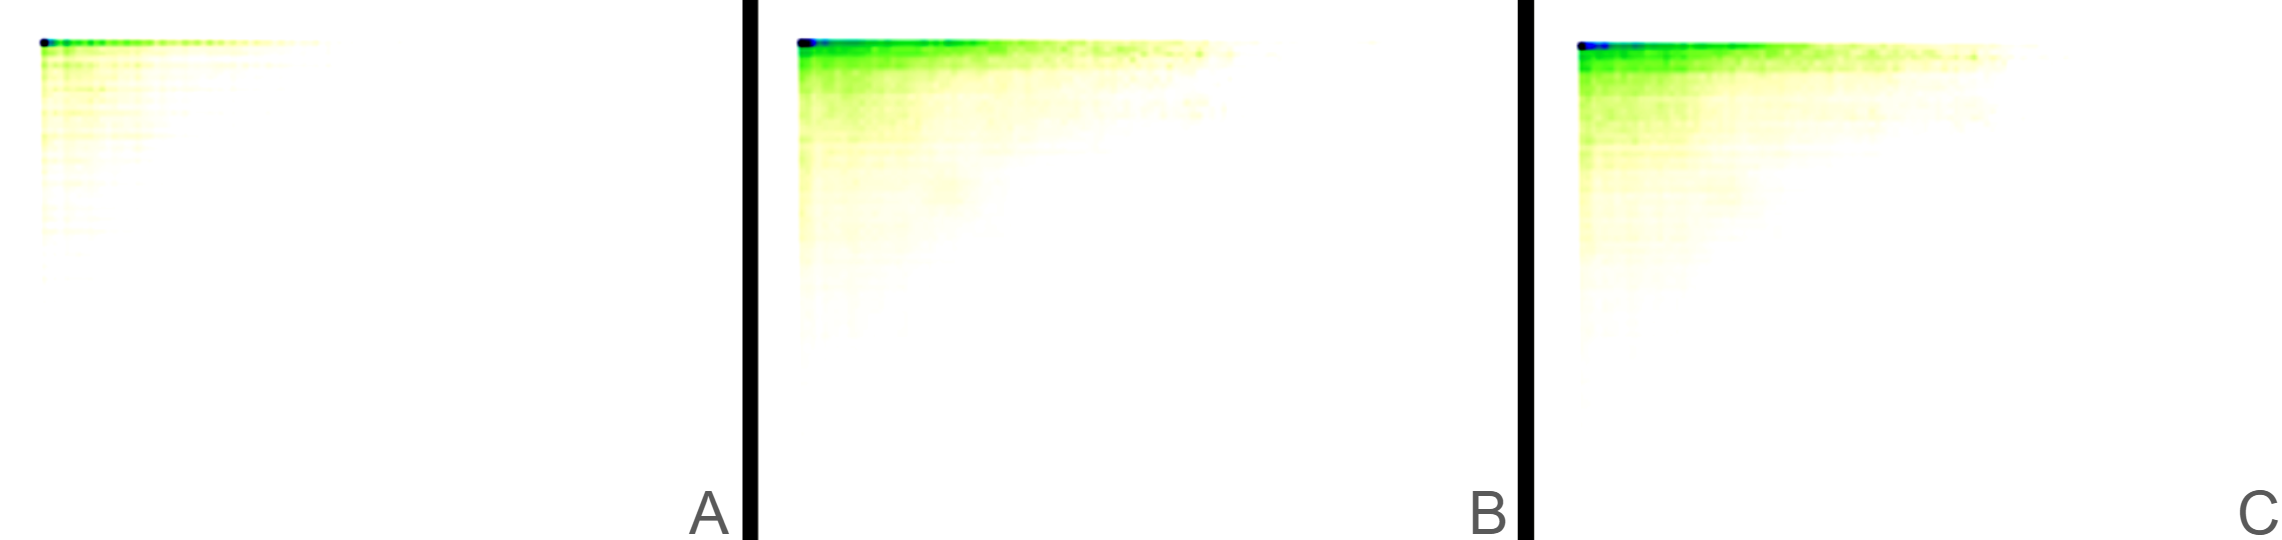
\includegraphics[width=0.92\textwidth]{figuras/xai.png}
    \fautor
\end{figure}

For Type classification, attributions often concentrate on structural bands,
indentation regions, and delimiter patterns. This is consistent with the idea
that file roles have visual structure. For Project classification, attributions
may highlight repository-specific conventions, headers, generated sections, or
boilerplate. For Author classification, attributions are more diffuse, suggesting
that stylistic signals are distributed and harder to localize.

These findings are valuable but also cautionary. If a Project classifier relies
heavily on boilerplate, it may not generalize to repositories with different
templates. If an Author classifier learns bot-generated patterns, it may not
represent human style. Explainability therefore serves as a check on the method,
not only as a defence of it.

\section{Study 3: Paired Anonymization Ablation}
\label{sec:study3-anonymization}

Because anonymization strips the lexical layer, the approach can be applied to
code that cannot leave an organization; the claim that it preserves predictive
utility therefore carries a large share of the proposal. Until recently that claim rested on a single
uncontrolled comparison. This section reports a controlled experiment designed
to replace it. It is a first instalment of Activity A2 rather than its
completion; the remaining scope is stated at the end of the section and in
Chapter~\ref{chapter:research-plan}.

\subsection{Design}

The experiment relies on a property of the method that makes the comparison
unusually direct. Anonymization is a deterministic per-character map applied
at rendering time: it changes pixel intensities and leaves geometry untouched.
The same source file can therefore be rendered twice, producing two images with
identical dimensions, identical layout and identical label, differing only in
the intensity alphabet. Both renderings are produced in a single pass, so the
two datasets are paired instance by instance. The pairing licenses paired
statistical tests, which are more sensitive than comparing two independent
runs.

The corpus is a large private enterprise system, a more recent version of one of
the projects used in the first study. Files were selected by extension, and only
textual source formats were read. Classes were defined by naming convention:
first by the suffix of the class name, and, when no suffix matched, by the
package the file belongs to. Keeping only classes with at least 300 examples and
capping each at 1,000 gives twelve classes and 10,927 paired minimaps, of which
10,923 pairs were usable. Descriptors are the same 59-bin LBP histograms used in
the first study.

The evaluation separates two questions that are routinely treated as one. The
first is whether any difference is detectable, and is answered by a paired
$t$-test over the cross-validation folds and by McNemar's test over paired
per-instance predictions \cite{mcnemar1947note}. The second is whether the
difference is small enough to be irrelevant, and is answered by two one-sided
tests of equivalence against a margin fixed before the experiment was run
\cite{schuirmann1987comparison}. The distinction matters: a non-significant
difference does not establish equivalence, since it may reflect nothing more
than lack of power. The equivalence margin was set at two percentage points of
accuracy. Both representations are evaluated on exactly the same splits of a
ten-times repeated five-fold stratified cross-validation, and the $t$-test uses
the correction of Nadeau and Bengio \cite{nadeau2003inference}, because folds of
a repeated cross-validation share training data and the uncorrected test is
anti-conservative.

\subsection{Results}

Table~\ref{tab:a2-anonymization} reports the outcome over fifty folds.

\begin{table}[ht]
\centering
\caption{Paired anonymization ablation with Random Forest over LBP descriptors,
twelve classes and 10,923 paired minimaps, ten times five-fold stratified
cross-validation. The difference is the accuracy lost by anonymizing.}
\label{tab:a2-anonymization}
\begin{tabular}{lc}
\toprule
\textbf{Measure} & \textbf{Value} \\
\midrule
Accuracy, original rendering & 0.8015 $\pm$ 0.0069 \\
Accuracy, anonymized rendering & 0.8076 $\pm$ 0.0063 \\
Difference (original $-$ anonymized) & $-$0.0060 \\
95\% confidence interval & [$-$0.0123, $+$0.0003] \\
Difference test (corrected paired $t$) & $p = 0.060$ \\
Equivalence within $\pm$0.02 (TOST) & $p = 2.4 \times 10^{-5}$ \\
\bottomrule
\end{tabular}
\fautor
\end{table}

Anonymization did not cost accuracy. The point estimate favours the anonymized
representation by 0.6 percentage points, and the confidence interval places the
largest loss compatible with the data at 0.0003, that is, at essentially zero.
The equivalence test rejects the hypothesis of a difference larger than the
declared margin.

The two tests should be read together rather than in isolation. The difference
test alone would support only the weak statement that no difference was
detected, at $p = 0.060$. The equivalence test supports the stronger and more
useful statement that the difference is bounded below the margin. McNemar's test
does find a detectable difference in six of the ten repetitions, and its
direction is consistent: across all repetitions, 5,239 instances were classified
correctly only by the anonymized representation against 4,580 only by the
original one. The result is therefore not that the two representations are
indistinguishable, but that the difference between them is small and, in this
setting, slightly favourable to anonymization.

A plausible explanation is that anonymization acts as a filter rather than only
as a loss. Collapsing letters and digits onto three intensities removes lexical
variation that a texture descriptor cannot exploit anyway, leaving the
structural skeleton more salient. The measurement in the next subsection
supports this reading.

\subsection{What the Transformation Removes}

The effect of anonymization on the representation can be quantified directly,
without training anything, because the map is deterministic. Measured over 12.3
million characters of the same corpus, the alphabet contracts from 152 to 37
distinct intensities and the entropy per pixel falls from 5.444 to 2.358 bits, a
reduction of 56.7\%. Only 25.9\% of characters survive unchanged, and those are
exactly the symbol classes: punctuation, delimiters and operators. The reduction
is uneven across file types, from 62.6\% for Java sources down to 48.0\% for SVG
files.

Read together, the two measurements say something that neither says alone: more
than half of the information carried by each pixel is discarded, and predictive
accuracy does not fall. That combination is evidence for the claim on which the
proposal rests, namely that the discriminative signal in a minimap is structural
rather than lexical. It also explains why the surviving 25.9\% is sufficient,
since block structure and layout are carried by punctuation and indentation.

\subsection{Scope of This Result}

Two boundaries must be respected when reading it. The evidence covers one
software system, so it establishes that anonymization can be cost-free, not that
it always is. And it covers one descriptor and one classifier family: Local
Binary Patterns describe local intensity relations, and may be constitutionally
blind to precisely the information that anonymization removes. A convolutional
model, which learns its own filters, could exploit lexical intensity differences
that LBP ignores, so this result does not transfer automatically to the
large-scale study of Section~\ref{sec:study2}. Extending the same protocol to
open-source corpora, to deep models, and to the Project and Author objectives is
the remainder of Activity A2.

\section{Artifact and Tool Results}

In addition to the two empirical studies, this work produced MinimapSignatures,
a multi-IDE tool ecosystem composed of a FastAPI/PyTorch inference backend, a
Visual Studio Code extension, and an IntelliJ IDEA plugin
\cite{gebara2026minimapsignatures}. The workflow was validated end-to-end: each
plugin generates an anonymized 128 by 128 minimap locally, submits it to the
backend, and displays ranked predictions for the Type, Project, and Author
targets. A fourth response target (quality) is a placeholder and currently
returns mock data; no model has been trained for it.

With this line of work, the thesis is no longer limited to a dataset-and-model
comparison; it also investigates how minimap analysis can become usable
infrastructure for software-engineering workflows. No user study
has been conducted yet, so the evaluation remains functional and
integration-oriented. The architecture, the deployed multitask model, the
current capture limits, and the validation status are detailed in
Chapter~\ref{chapter:tool-support}.

\section{Consolidated Evidence}

Table~\ref{tab:preliminary-evidence} summarizes the evidence produced so far and
how it supports the research questions.

\begin{table}[ht]
\centering
\caption{Preliminary evidence and relation to research questions.}
\label{tab:preliminary-evidence}
\begin{tabular}{p{0.24\textwidth}p{0.43\textwidth}p{0.18\textwidth}}
\toprule
\textbf{Evidence} & \textbf{Main finding} & \textbf{Related RQs} \\
\midrule
LBP study & Minimap texture supports software-feature classification with Random Forest near 93\% accuracy. & RQ1, RQ2 \\
Fixed-size comparison & 128 by 128 minimaps remain competitive with variable-size minimaps. & RQ1, RQ2 \\
Large-scale dataset & Minimap learning scales to 685,906 images from 100 projects and 10 languages. & RQ1 \\
Deep learning results & EfficientNet-B0 pretrained reaches strong validation results for Type, Project, and Author. & RQ1, RQ2 \\
Integrated Gradients & Different objectives rely on different visual regions and patterns. & RQ3 \\
MinimapSignatures & IDE plugins and backend validate an end-to-end tool workflow. & RQ5 \\
\bottomrule
\end{tabular}
\fautor
\end{table}

The evidence supports continuing the doctoral research, but it also defines the
remaining challenges. The next phase must deepen the evaluation of
anonymization, improve imbalance-aware learning, refine dataset splits, extend
the task set toward quality and architectural analysis, and evaluate the tool
with developers or realistic development scenarios.

\section{Interpretation by Research Question}

The preliminary studies already provide partial answers to the research
questions stated in the Introduction.

\subsection{RQ1: Discriminative Structural Cues}

The LBP study and the large-scale deep learning study both support the idea that
minimaps preserve discriminative structural cues. In the first study, the
success of Random Forest over LBP histograms indicates that texture-level
information is meaningful. In the second study, the strong Type classification
results indicate that fixed-size minimaps preserve enough information to
distinguish many artifact categories across a much larger corpus. Together,
these results support the representational premise of the work: the
two-dimensional layout of source files carries a signal that survives both
compression to 128 by 128 pixels and lexical suppression, and that would not be
directly visible to models consuming code as a one-dimensional sequence.

However, RQ1 is not fully answered. The current evidence is strongest for the
datasets already used. Future work must evaluate additional repositories,
stronger splits, and quality-related tasks. It must also examine which classes
are consistently difficult and whether failures are due to representation loss,
label ambiguity, or insufficient samples.

\subsection{RQ2: Handcrafted and Learned Representations}

The first study shows that handcrafted texture descriptors are a viable
baseline. The second study shows that deep models can operate directly on
minimap images at scale. The comparison suggests that handcrafted descriptors
are useful for simpler settings, while learned representations become important
when the dataset is larger, more imbalanced, and more heterogeneous.

The remaining work should compare these pipelines under the same dataset
conditions. For example, LBP histograms can be computed for the large-scale
dataset and compared with deep models under identical splits. This would make
the answer to RQ2 more precise.

\subsection{RQ3: Visual Evidence and Explainability}

Integrated Gradients provides an initial answer to RQ3. The attribution maps
suggest that models use structural bands, boilerplate regions, and diffuse style
patterns depending on the objective. This supports the claim that predictions
are not arbitrary, but it also reveals risks. If a model depends too strongly on
headers or generated sections, then its performance may reflect dataset
artifacts rather than genuine software structure.

Future work must make this analysis more systematic. Instead of inspecting only
representative examples, the thesis should aggregate attribution statistics,
compare attribution patterns across classes, and perform ablation experiments
that remove or mask salient regions.

\subsection{RQ4: Anonymization}

The paired ablation of Section~\ref{sec:study3-anonymization} answers this
question directly for one system. Over twelve classes and 10,923 paired
minimaps, anonymization did not reduce accuracy: the difference was $-0.0060$ in
favour of the anonymized representation, with a 95\% confidence interval whose
upper bound is 0.0003, and equivalence within two percentage points holds at
$p = 2.4 \times 10^{-5}$. The result is reinforced by the measurement of the
transformation itself, which discards 56.7\% of the entropy per pixel while
leaving accuracy intact. An earlier comparison made during the first study
pointed in the same direction, with average F1-score falling from 0.83 to 0.82
for an SVM over ten classes \cite{gebara2025iwssip}, though that figure came
from a single uncontrolled run.

This evidence matters for two reasons.

First, it indicates that the discriminative signal resides in structural
features such as indentation patterns, operator density, punctuation layout,
and block organization, rather than in identifier names or literal values. The
model does not appear to need lexical content to distinguish file types,
project origins, or authorship styles.

Second, it supports the industrial motivation developed in
Chapter~\ref{chapter:foundations}: if anonymization preserves utility, an
organization can submit anonymized minimaps to an external analysis service
while the business logic embedded in the lexical layer stays local.

The Author objective matters here. Style remains identifiable after full
lexical suppression, which is direct evidence that the model operates on
structural patterns; if author identification depended on lexical content,
anonymization would have eliminated it.

A formal ablation study is still required. The thesis should repeat the
comparison under documented conditions, cover multiple suppression levels,
measure degradation curves, and characterize what remains inferable from
anonymized minimaps under each strategy (Activity A2 in
Chapter~\ref{chapter:research-plan}).

\subsection{RQ5: IDE Integration}

MinimapSignatures provides an initial answer to RQ5 by showing that minimap
analysis can be integrated into Visual Studio Code and IntelliJ IDEA. The
functional validation confirms that the technical workflow is feasible.

However, developer usefulness remains open. The current prototype shows that
predictions can be delivered inside IDEs, but it does not prove that developers
benefit from them. Future work must evaluate whether the feedback is
understandable, whether explanations increase trust, and whether multi-file
analysis is more useful than single-file prediction.

\section{Limitations of the Current Evidence}

The current evidence has several limitations. First, the first study uses a
limited dataset compared with the later corpus. Its results are valuable as
proof of feasibility, but they should not be generalized beyond the evaluated
setting without further experiments.

Second, the large-scale study is affected by class imbalance. Strong accuracy
and ROC-AUC values show that the models learn substantial signal, but they do
not guarantee equally strong behavior for minority classes. Macro-F1, per-class
recall, and confusion matrices must be emphasized in the thesis.

Third, the Author objective must be interpreted carefully. Labels may reflect
last committers, bots, project maintainers, or generated artifacts, which
introduces noise. Methodologically, the objective serves as a probe: it tests
whether style-related structural patterns survive anonymization. In this role it
is valuable. However, the objective is not presented as a deployment-ready
author identification tool, and the thesis should be explicit about this
distinction.

Fourth, the current tool evaluation is functional. It confirms that the
architecture works, but it does not measure usability, usefulness, or impact on
developer productivity. This distinction must be preserved in the thesis.

Finally, the current studies focus mostly on classification. The most valuable
software-engineering applications may require ranking, anomaly detection,
clustering, explanation, or integration with other signals. These directions
remain to be explored.

\section{Implications for the Thesis}

The preliminary results shape the final thesis in a concrete way. The thesis
does not need to prove from scratch that minimaps contain information; the early
studies already support that claim. Instead, the thesis must characterize that
information: how far it generalizes, how it can be interpreted, and what it is
useful for.

This shifts the emphasis from simple feasibility to disciplined evaluation. The
next experiments should ask harder questions: whether the representation
generalizes across repositories, whether minority classes are handled fairly,
whether anonymization is strong enough, whether explanations reveal meaningful
evidence, and whether developers can use the feedback in realistic tasks.

The final thesis should therefore be organized around a progression:
representation, evidence, interpretation, and operationalization. The current
chapter provides the evidence base for that progression.


\chapter{MinimapSignatures: Tool Support}
\label{chapter:tool-support}
\section{Motivation for Tool Support}

Research artifacts in software engineering become more valuable when they can be
used in realistic workflows. A model that classifies minimap images in an
offline experiment demonstrates feasibility, but developers work inside IDEs,
version-control systems, code-review platforms, and continuous-integration
pipelines. Therefore, one of the objectives of this doctoral project is to
connect minimap-based analysis to practical development environments.

The tool-support line is named \textit{MinimapSignatures}. Its purpose is to
operationalize source code minimaps as visual signatures inside IDEs. The tool
does not replace syntax highlighting, code navigation, static-analysis warnings,
or dependency inspection. Instead, it adds a model-based visual-analysis layer:
the active source file is transformed into an anonymized minimap, sent to a
backend, classified by trained models, and returned to the IDE as developer-facing
feedback.

This tool line contributes to the thesis in three ways. First, it validates that
minimap generation can be executed locally in development environments. Second,
it shows that the same backend contract can support different IDE clients.
Third, it creates infrastructure for future evaluations involving multi-file
analysis, project-specific models, code quality indicators, and developer
feedback.

\section{Architecture}

MinimapSignatures follows a client--server architecture. The clients are IDE
plugins for Visual Studio Code and IntelliJ IDEA. The server is a Python backend
responsible for receiving minimap images, preprocessing them, invoking trained
models, and returning structured predictions. Figure~\ref{fig:tool-architecture}
illustrates the architecture.

\begin{figure}[ht]
    \centering
    \caption{Architecture of the MinimapSignatures ecosystem.}
    \label{fig:tool-architecture}
    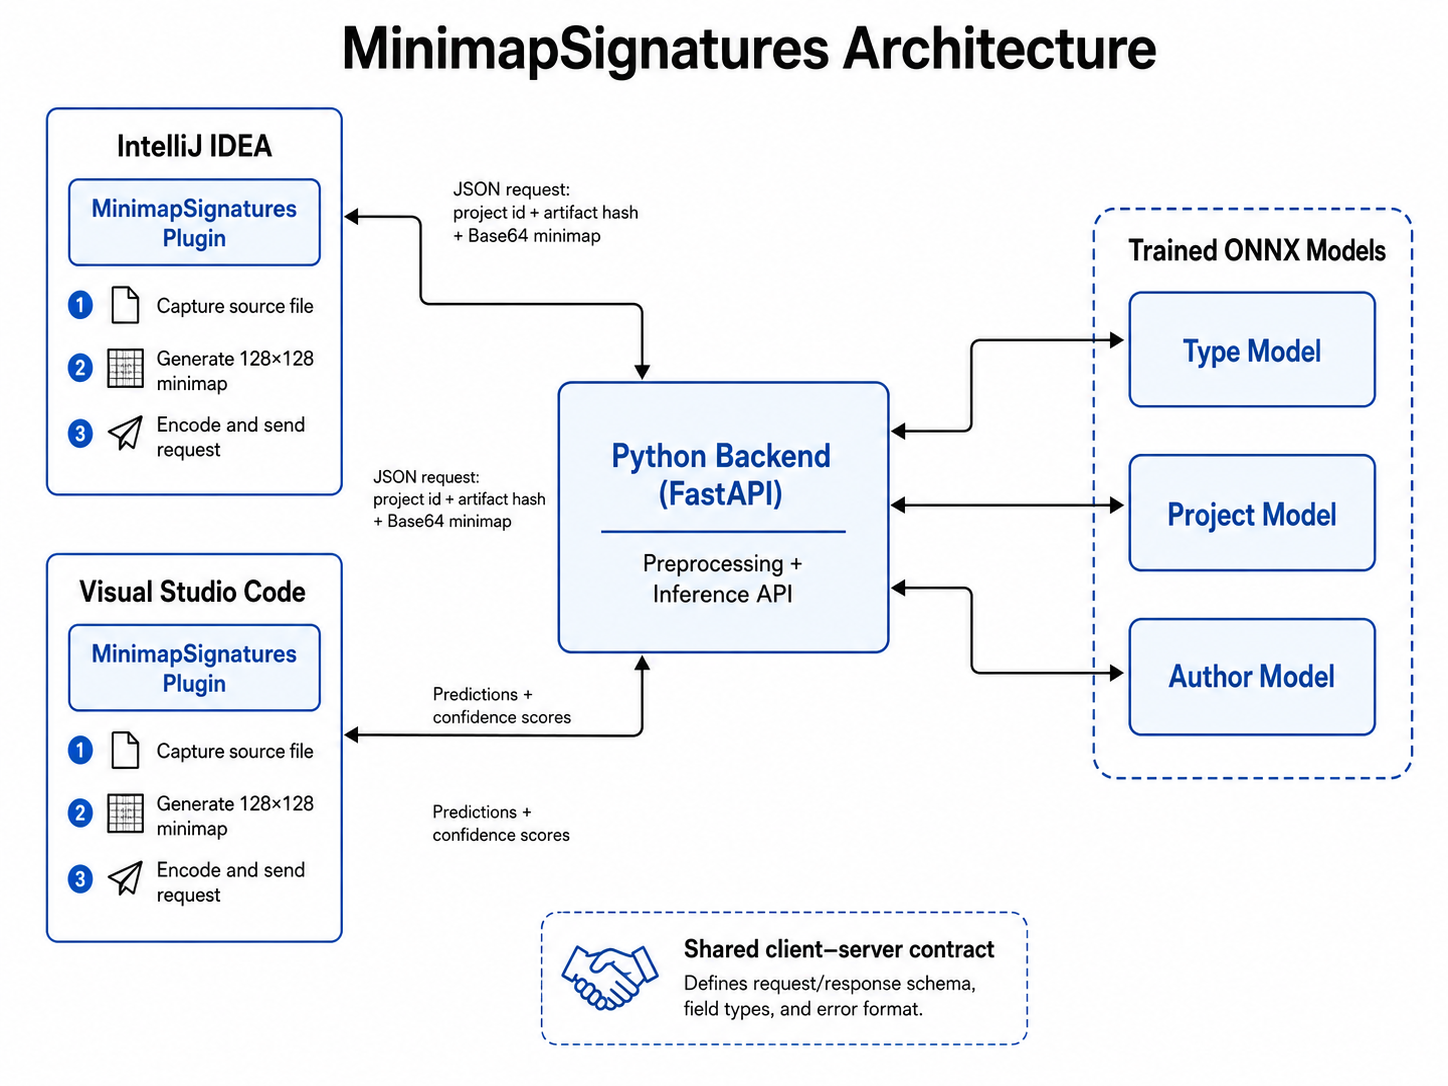
\includegraphics[width=0.92\textwidth]{figuras/minimapsignatures-architecture.png}
    \fautor
\end{figure}

The separation between clients and backend is a central design decision. IDE
plugins should remain lightweight because each IDE has its own APIs, packaging
requirements, and interaction patterns. Model inference, on the other hand, may
change frequently as new architectures, datasets, and objectives are introduced.
By decoupling them, the project can update the backend without rewriting each
plugin.

\section{Backend Service}

The backend is implemented in Python and exposes an HTTP interface. Its main
endpoint receives a JSON payload containing metadata and a base64-encoded PNG
image representing the minimap. The backend decodes the image, converts it to
the expected grayscale format, normalizes pixel values, invokes the trained
models, and returns prediction groups.

The backend is designed around the prediction objectives used in the large-scale
study: Type, Project, and Author. This does not mean that every deployment must
use all three objectives. In practice, Type is the most immediately useful and
least ethically sensitive target. Project can support repository-convention
analysis. Author should be treated cautiously and may be disabled or reframed as
style analysis in many contexts.

The backend design supports model evolution. A future version may add
quality-related models, code-smell indicators, architectural-deviation scores,
or explanation maps. Since the clients communicate through a shared contract,
these new results can be added as new response fields or prediction groups.

\section{Visual Studio Code Extension}

The Visual Studio Code extension provides a graphical WebView interface. When a
developer triggers the analysis, the extension captures the active file,
generates an anonymized 128 by 128 minimap, sends it to the backend, and displays
the returned predictions. The WebView can show the minimap image, artifact hash,
prediction groups, confidence values, and later explanation overlays.

Figure~\ref{fig:vscode-plugin} shows the Visual Studio Code interface.

\begin{figure}[ht]
    \centering
    \caption{Visual Studio Code extension showing minimap analysis results.}
    \label{fig:vscode-plugin}
    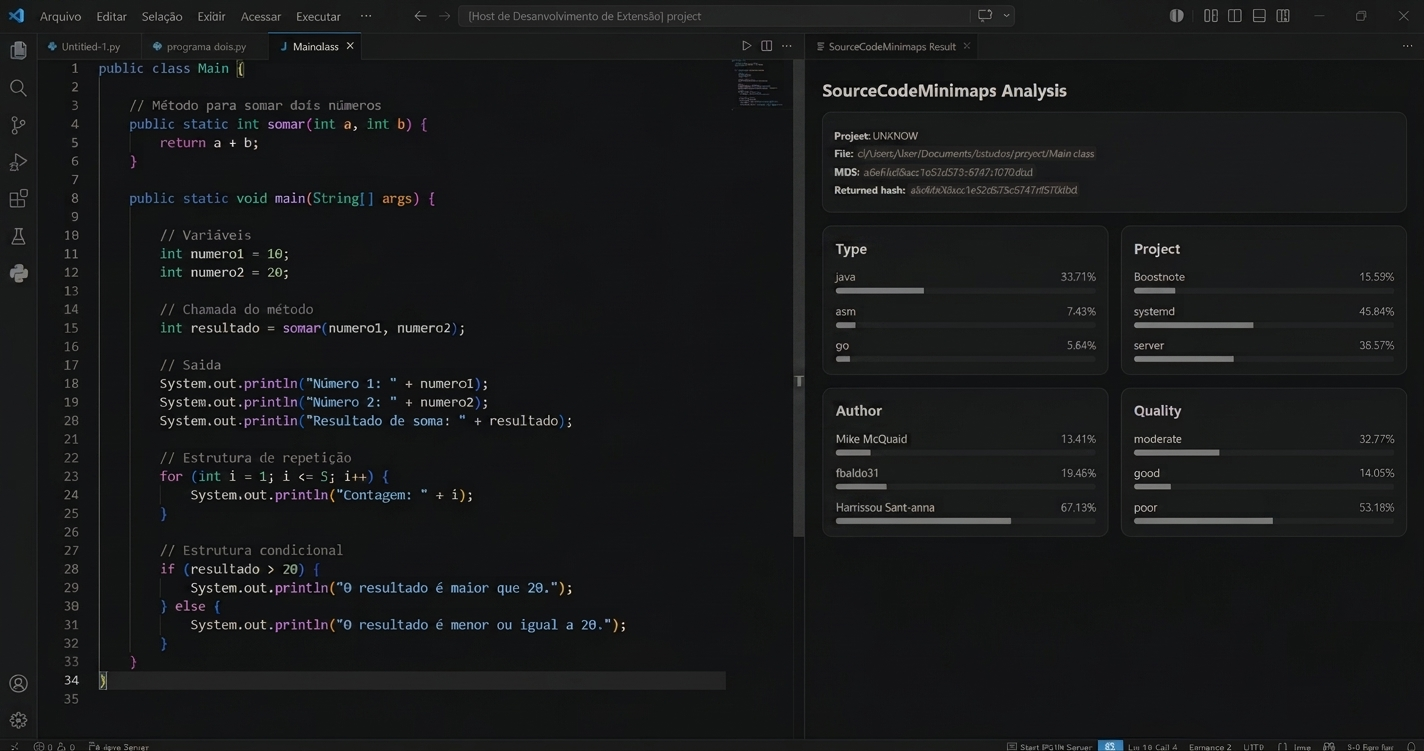
\includegraphics[width=0.92\textwidth]{figuras/vscode-plugin.png}
    \fautor
\end{figure}

The WebView approach is useful for richer visual feedback. It can present cards,
confidence bars, minimap images, and future XAI overlays. This makes it suitable
for exploratory workflows in which a developer wants to inspect files, folders,
or project-level patterns.

\section{IntelliJ IDEA Plugin}

The IntelliJ IDEA plugin follows a lighter interaction model. It captures the
active source artifact, generates the minimap, sends it to the backend, and
displays a Markdown-based report in a split-screen editor. This approach
integrates naturally with the IDE because the result appears as a document beside
the source file.

Figure~\ref{fig:intellij-plugin} shows the IntelliJ IDEA plugin interface.

\begin{figure}[ht]
    \centering
    \caption{IntelliJ IDEA plugin displaying a Markdown report generated from minimap analysis.}
    \label{fig:intellij-plugin}
    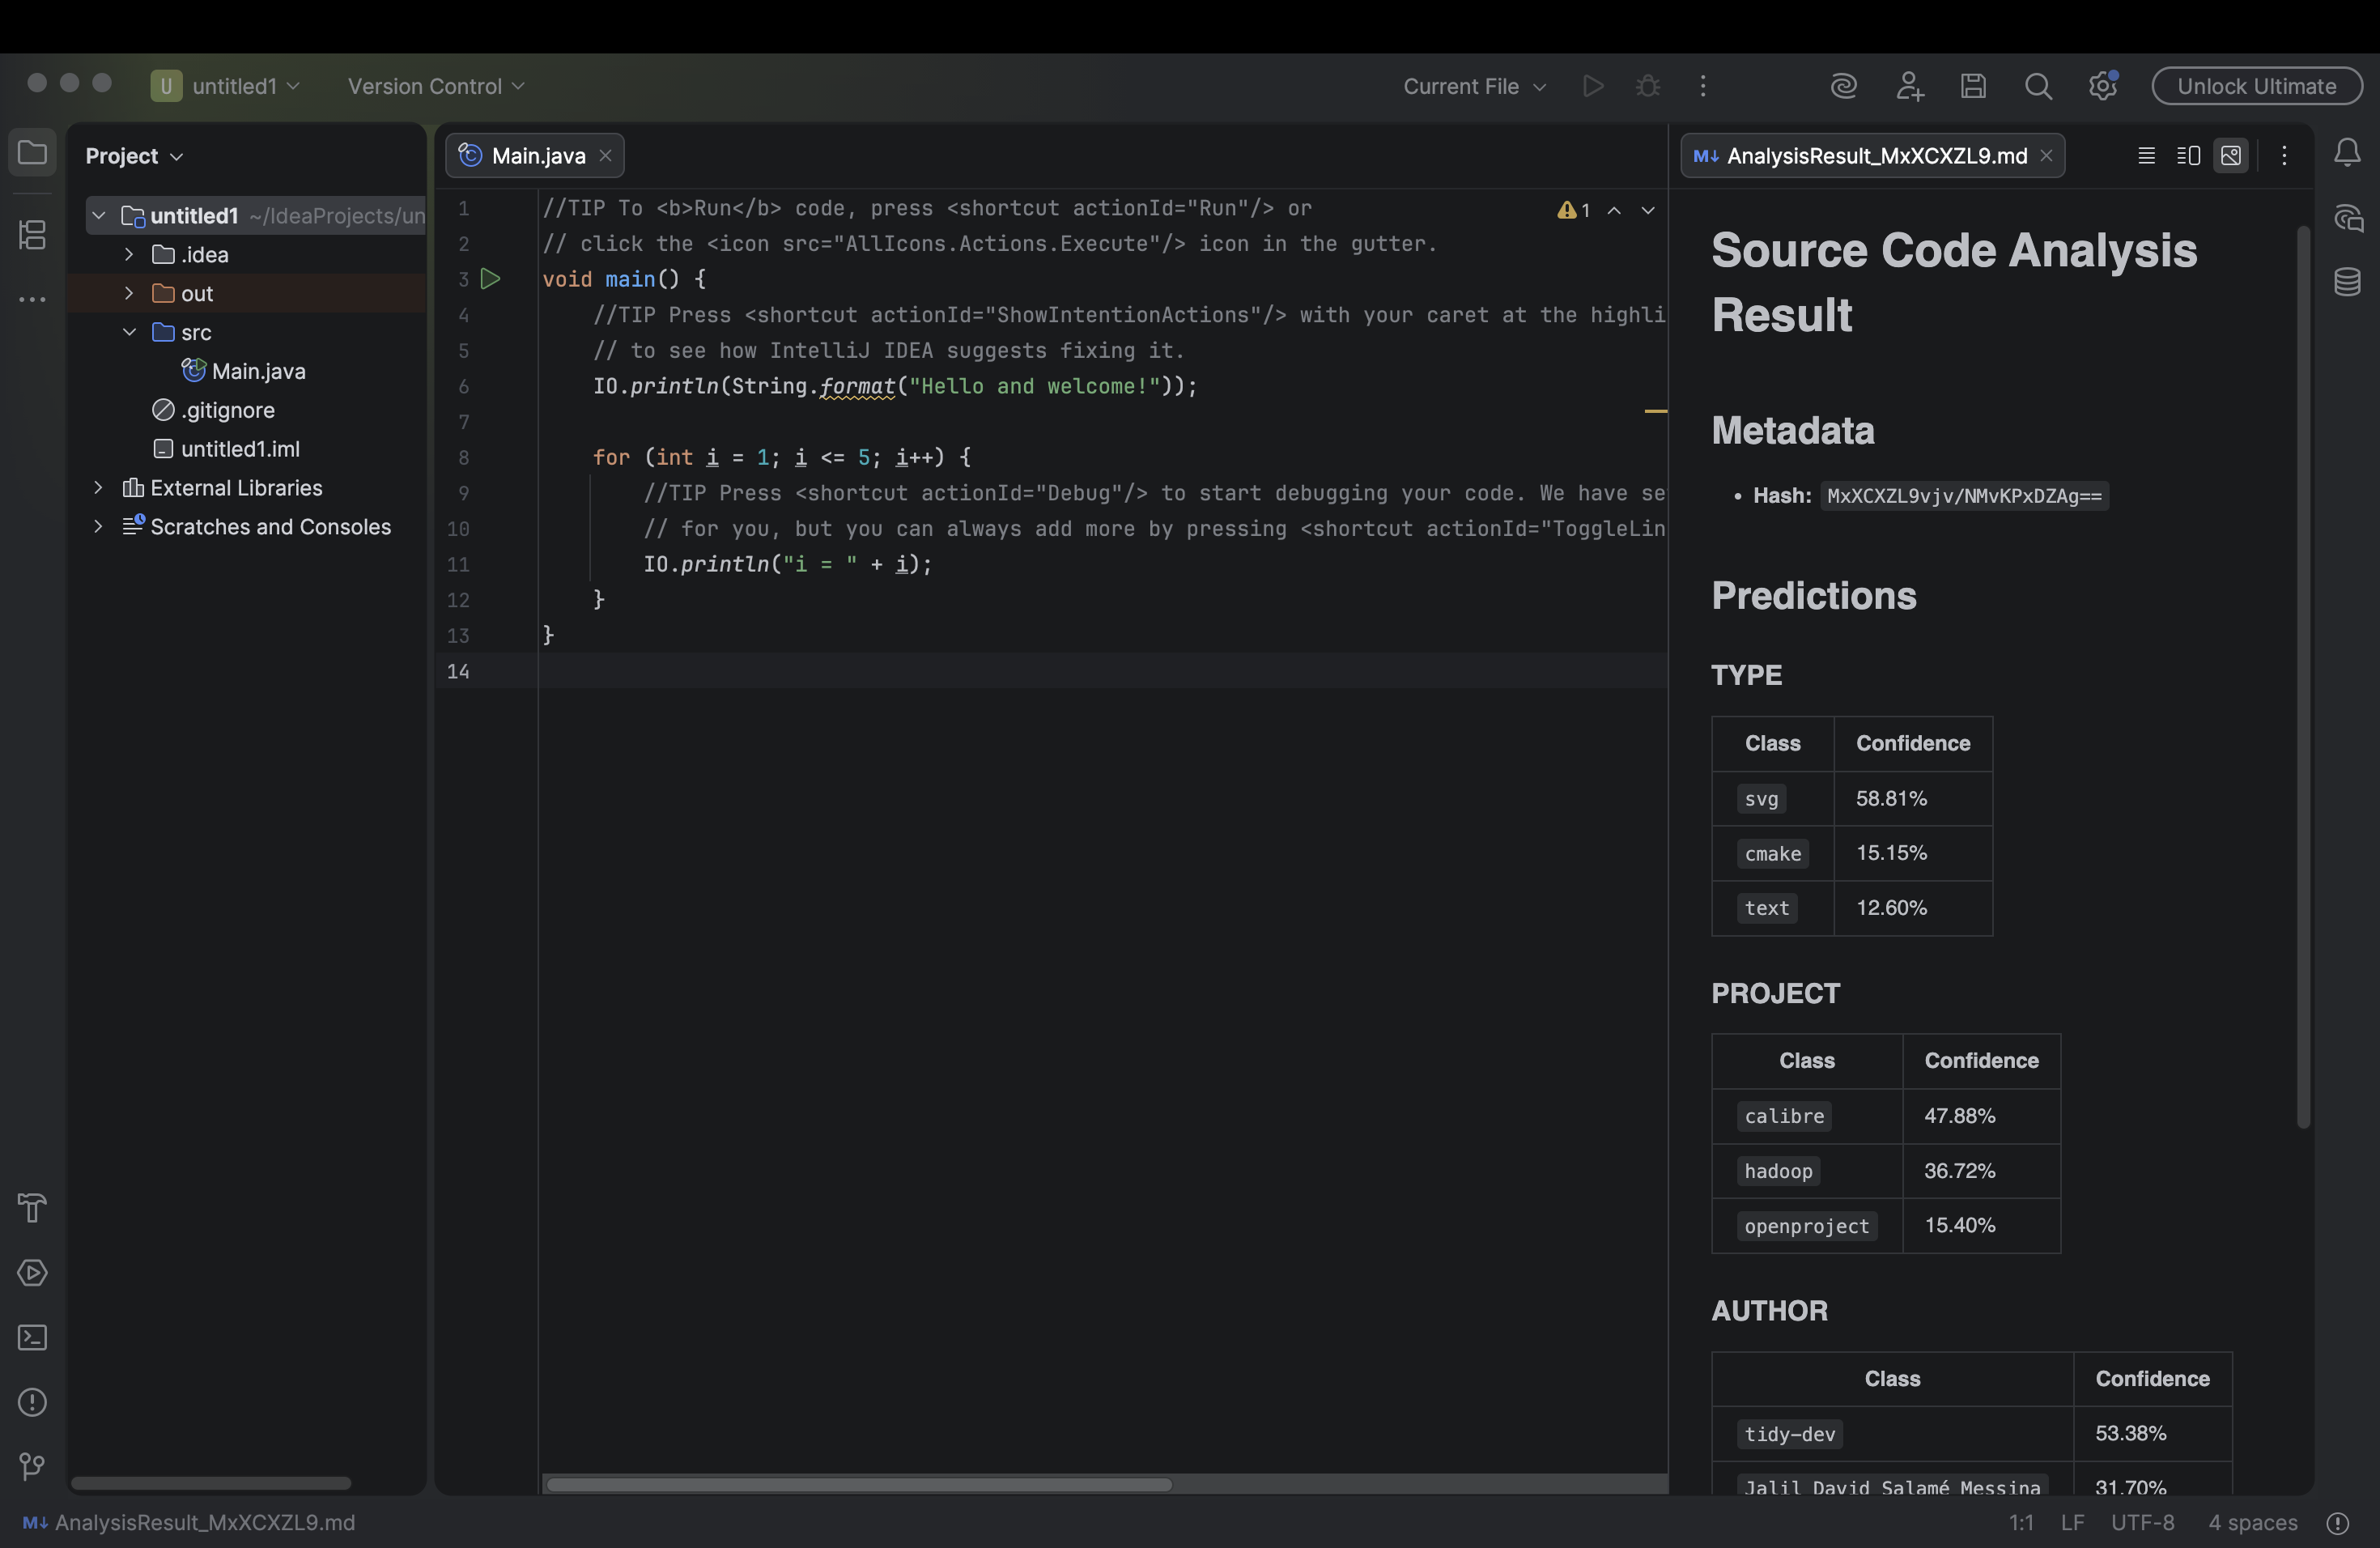
\includegraphics[width=0.92\textwidth]{figuras/intellij-plugin.png}
    \fautor
\end{figure}

The Markdown approach is less visually elaborate than the WebView interface, but
it is simple, robust, and aligned with quick inspection. It also produces a
textual artifact that can be saved, shared, or attached to later analysis.

\section{Shared Client--Server Contract}

Both IDE clients follow the same conceptual contract. Table~\ref{tab:tool-contract}
summarizes the main request and response elements.

\begin{table}[ht]
\centering
\caption{Shared client--server contract in MinimapSignatures.}
\label{tab:tool-contract}
\begin{tabular}{p{0.22\textwidth}p{0.58\textwidth}}
\toprule
\textbf{Element} & \textbf{Description} \\
\midrule
Project identifier & Optional or inferred identifier for the current workspace. \\
Artifact hash & Stable hash used to identify the analyzed file without sending its path in clear text. \\
Minimap image & Base64-encoded PNG generated locally by the IDE client. \\
Model group & Prediction target such as Type, Project, or Author. \\
Predicted label & Most likely class returned by the backend. \\
Confidence score & Numeric score associated with the prediction. \\
Additional metadata & Optional fields for model version, preprocessing mode, or explanation data. \\
\bottomrule
\end{tabular}
\fautor
\end{table}

The shared contract confirms that minimap-based analysis is not tied to a single
IDE. Additional clients can be implemented by generating the same minimap format
and sending the same request structure.

\section{Functional Validation}

The current evaluation of MinimapSignatures is functional and
integration-oriented. It verifies whether the complete workflow can be executed
successfully. Table~\ref{tab:functional-validation} summarizes the validation
status.

\begin{table}[ht]
\centering
\caption{Functional validation of MinimapSignatures.}
\label{tab:functional-validation}
\begin{tabular}{p{0.58\textwidth}p{0.20\textwidth}}
\toprule
\textbf{Component or feature} & \textbf{Status} \\
\midrule
Backend receives base64 minimap payloads & Validated \\
Backend preprocesses images for inference & Validated \\
Backend invokes trained models & Validated \\
Backend returns structured prediction groups & Validated \\
Visual Studio Code extension generates and submits minimaps & Validated \\
Visual Studio Code extension displays WebView results & Validated \\
IntelliJ IDEA plugin generates and submits minimaps & Validated \\
IntelliJ IDEA plugin displays Markdown results & Validated \\
Shared client--server contract works across IDEs & Validated \\
Multi-file and project-level analysis & Planned \\
Project-specific model update & Planned \\
Developer usability evaluation & Planned \\
\bottomrule
\end{tabular}
\fautor
\end{table}

This validation does not yet demonstrate that the tool improves productivity,
reduces comprehension effort, or increases trust. Those claims require a
different evaluation design, such as observational studies, controlled tasks,
interviews, or field deployments. At this stage, the contribution is that the
research pipeline can be executed from real IDEs.

\section{Usage Scenarios}

MinimapSignatures can support several usage scenarios. The current prototype
implements only part of them, but they guide future development and evaluation.

\subsection{Single-File Inspection}

In the simplest scenario, a developer opens a file and triggers minimap analysis.
The tool returns the predicted Type, optional Project or style-related
predictions, confidence scores, and later an explanation overlay. This scenario
is useful when a developer inspects an unfamiliar file and wants a quick
classification or when a reviewer wants to compare a file against expected
roles.

\subsection{Code Review Support}

During code review, a pull request may introduce files that visually differ from
the existing project conventions. A minimap-based tool could flag unusual
artifacts for additional inspection. The output should be framed carefully: the
tool should not say that a file is wrong, but that it is visually unusual
relative to a learned distribution. This makes the tool a prioritization aid.

\subsection{Onboarding and Repository Exploration}

A new developer entering a project often needs to understand file roles and
project organization. A project-level version of MinimapSignatures could render
minimaps for selected folders, group similar artifacts, and summarize dominant
file patterns. Such a view would complement textual navigation and dependency
analysis.

\subsection{Project-Specific Model Adaptation}

Organizations may have conventions that differ from open-source datasets. A
future version of the tool could allow teams to generate a private minimap
catalog and train or fine-tune project-specific models. This would make the
analysis more relevant to local architecture, naming patterns, and quality
expectations, while still avoiding transmission of raw source code.

\section{Artifact Availability and Repositories}

The public code organization for the project is
\url{https://github.com/minimap-project}. At the time this document was prepared,
the organization included repositories for the training infrastructure,
shared assets, backend service, IntelliJ IDEA plugin, and Visual Studio Code
extension. The artifact structure supports separation of concerns:

\begin{itemize}
    \item \texttt{minimap-signatures-trainer}: training and model-related code;
    \item \texttt{assets}: shared visual and documentation assets;
    \item \texttt{back-end}: Python inference backend;
    \item \texttt{intellij-plugin}: IntelliJ IDEA client;
    \item \texttt{vscode-plugin}: Visual Studio Code client.
\end{itemize}

This organization is useful for research reproducibility because it avoids
mixing IDE-specific code with training scripts and backend inference logic. It
also allows each component to evolve independently. For example, a new model can
be added to the backend without changing the extension packaging, while a new
IDE client can reuse the same backend contract.

\section{Planned Extensions}

The next versions of MinimapSignatures should support four extensions.

First, the tool should move from single-file analysis to multi-file and
project-level analysis. This would allow developers to inspect a folder, module,
or entire repository and receive summaries of visual signatures, unusual files,
or clusters of similar artifacts.

Second, the backend should support explanation maps. Integrated Gradients or
other attribution methods can be computed server-side and returned to the IDE so
that developers can see which regions influenced predictions. This would make
the tool more transparent than a label-only classifier.

Third, the tool should support project-specific model customization. A team may
want to train or adapt a model using its own conventions, especially for
architectural roles or quality indicators. The minimap catalog and backend
architecture can support this direction.

Fourth, the tool should include quality-related targets. Instead of predicting
only Type, Project, or Author, future models may identify code-smell likelihood,
architectural deviation, generated-file anomalies, suspicious templates, or
files that deserve priority in code review.

These extensions will move the tool from proof of integration toward a research
platform for developer-facing visual source code analysis.


\chapter{Research Plan, Risks, and Threats to Validity}
\label{chapter:research-plan}
This chapter turns the evidence gathered so far into a plan for the remainder of
the doctorate. It begins by stating what has already been produced and what is
therefore no longer at risk, and derives from that the deliverables the thesis
must still provide. The planned activities, experiments, and evaluation criteria
follow, each connected to the gaps identified in the previous chapters. The
chapter then addresses the conditions under which the work must be carried out,
namely the threats to the validity of the results, the responsible use of author
prediction, the open science commitments, the project risks, and the schedule
that fits the remaining time before the defense.

\section{Current Status}

At the qualification stage, this work has already produced three
main outputs. The first is an initial empirical study on source code minimaps,
Local Binary Patterns, and traditional classifiers \cite{gebara2025iwssip}. The
second is a large-scale study with 685,906 minimaps from 100 open-source
projects and 10 programming languages \cite{gebara2025ciarp}. The third is the
MinimapSignatures tool ecosystem, which validates the feasibility of bringing
minimap analysis into IDE workflows \cite{gebara2026minimapsignatures}. To these
is added an unpublished result produced for this document: the paired
anonymization ablation of Section~\ref{sec:study3-anonymization}, which gives
the confidentiality claim of the proposal a measured basis it previously
lacked.
Table~\ref{tab:publications} summarizes this production and its editorial
status; the three completed articles are reproduced in
Appendices~\ref{apendice:iwssip} to~\ref{apendice:sbes}.

\begin{table}[ht]
\centering
\caption{Scientific production associated with this doctoral research.}
\label{tab:publications}
\begin{tabular}{p{0.40\textwidth}p{0.20\textwidth}p{0.11\textwidth}p{0.13\textwidth}}
\toprule
\textbf{Paper} & \textbf{Venue} & \textbf{Role} & \textbf{Status} \\
\midrule
Software Feature Detection Using Source Code Minimaps as Visual Signatures \cite{gebara2025iwssip} & IWSSIP 2025 (IEEE) & Main author & Published \\
Source Code Minimaps at Scale: Feature-Oriented Analysis of 100 Projects \cite{gebara2025ciarp} & CIARP 2025 (Springer LNCS 16528) & Main author & Published \\
MinimapSignatures: A Multi-IDE Ecosystem for Analysis of Visual Source Code Signatures \cite{gebara2026minimapsignatures} & SBES-Tools 2026 (CBSoft) & Main author & Accepted \\
\midrule
Explainability of visual code representations (working title) & VISAPP 2027 & Main author & Planned \\
Consolidated study on confidentiality-preserving visual code analysis (working title) & Empirical Software Engineering & Main author & Planned \\
\bottomrule
\end{tabular}
\fautor
\end{table}

The last two rows are targets, not results. The proceedings volume of CIARP
2025 appeared in 2026, which is the year recorded in the corresponding
bibliography entry. VISAPP 2027 is the venue
chosen for the explainability work developed during the research internship
abroad described in Section~\ref{sec:internship}: it is a computer vision
conference whose scope covers representation learning and texture analysis,
which matches the framing of this research, and its schedule aligns with the
internship, with a regular paper deadline expected for September 2026 according
to the current call, and the conference held in February 2027. The journal target is \emph{Empirical Software
Engineering}, chosen because the final contribution is an empirical study of a
software engineering problem rather than a purely methodological result, and
because the venue expects the kind of controlled evaluation and reproducibility
package that this work plans to deliver. The submission is planned for the
second half of 2027, once repository-disjoint evaluation and the anonymization
ablation are complete, so that the article reports consolidated evidence
instead of preliminary results.

These outputs establish a solid foundation, but the thesis is not complete. The
remaining work must deepen the methodology, broaden the task set, strengthen
evaluation, and connect the tool to developer-facing scenarios. This chapter
defines the planned research activities and the main risks.

\section{Expected Deliverables}

The final doctoral work is expected to produce a set of deliverables, not a
single isolated experiment. The main deliverables are:

\begin{enumerate}
    \item a finalized methodology for source code minimap generation,
    anonymization, cataloging, and evaluation;
    \item a curated and documented minimap dataset or dataset-generation package;
    \item benchmark results comparing handcrafted descriptors and deep visual
    models under controlled splits;
    \item an anonymization study measuring the trade-off between information
    suppression and predictive performance;
    \item an explainability study showing which visual regions support model
    decisions;
    \item an extended MinimapSignatures prototype with multi-file or
    explanation-oriented feedback;
    \item at least one evaluation of developer-facing use, even if exploratory;
    \item the final thesis text and associated reproducibility package.
\end{enumerate}

The deliverables depend on one another: the dataset and methodology feed the
models, the models feed the explanation protocols, and the explanations become
the tool feedback that the developer-centered evaluation will assess.

\section{Remaining Research Activities}

The remaining doctoral work is organized into six activities.

\subsection{A1: Refined Dataset Curation}

The large-scale dataset must be refined for additional experiments. This
includes improving label hygiene, identifying generated files, separating bot and
human contributors when possible, recording repository metadata, and creating
balanced or task-specific subsets. The catalog should support reproducible
filtering decisions.

This activity is necessary because the current dataset is large but imbalanced.
Head classes dominate some objectives, and Author labels may contain bots,
organizations, or aliases. Bots are pervasive in popular open-source projects:
about a quarter of popular GitHub repositories use them \cite{wessel2018power},
so bot-authored files are likely present in a corpus selected by popularity.
Planned curation heuristics include matching author names against known bot
naming patterns (such as the \texttt{[bot]} suffix), merging aliases by
normalized name and e-mail, and flagging accounts with anomalous commit volume
for manual inspection. The proportion of bot-attributed files will be reported,
and Author experiments will be run with and without these accounts. Better
curation will make later experiments more trustworthy.

\subsection{A2: Anonymization Evaluation}

The first installment of this activity is already complete and is reported in
Section~\ref{sec:study3-anonymization}. A paired ablation over twelve classes
and 10,923 minimaps of a large government system found no accuracy cost for
anonymization, with equivalence within two percentage points established at
$p = 2.4 \times 10^{-5}$, while the transformation itself removes 56.7\% of the
entropy per pixel. That experiment retires the uncontrolled comparison on which
the confidentiality argument previously rested, and its instruments, paired
generation, repeated cross-validation on shared splits, McNemar's test and an
equivalence test against a pre-declared margin, are reused unchanged in what
follows.

Three boundaries of that result define the remaining work. It covers a single
software system, so the ablation must be repeated on the open-source corpus,
where the dataset can also be published for external replication. It covers a
single descriptor and classifier: Local Binary Patterns may be insensitive to
exactly what anonymization removes, so the comparison must be repeated with the
convolutional backbones of the large-scale study, which learn their own filters.
And it covers only the Type objective, so Project and Author must be evaluated
as well, the latter being the objective most likely to depend on suppressed
content.

Beyond replicating the two-level comparison in these settings, Activity A2 will
extend it into a graded study over several suppression levels:

\begin{itemize}
    \item baseline (the current character-to-pixel mapping: letters and digits
    replaced by canonical values, other characters kept as raw ASCII);
    \item no anonymization (raw character codes, including identifiers and literals);
    \item comment removal (strip comment regions before rendering);
    \item punctuation normalization (map all operators and delimiters to a single
    canonical value, testing whether structure beyond punctuation still carries signal);
    \item maximum suppression (all non-whitespace characters to a single value,
    preserving only blank lines and indentation).
\end{itemize}

To avoid post hoc rationalization, the ablation design is declared in this
proposal, before execution. All suppression levels will share identical
repository-aware splits, seeds, architecture, and training budget, so that the
anonymization level is the only manipulated factor. The primary metric is
macro-F1 per objective; accuracy and per-class recall are secondary. Every
comparison against the non-anonymized rendering will be reported with both a
difference test and an equivalence test, since a non-significant difference on
its own would establish nothing. The equivalence margin remains two percentage
points, the value used and declared in the completed installment. A drop beyond
that margin will be reported as a negative result and will trigger a revision of
the confidentiality claims made in this proposal. Results for all levels will be reported regardless of outcome, and
the goal remains a performance-versus-suppression trade-off curve indicating
which level is appropriate when intellectual property protection is the
primary concern.

\subsection{A3: Imbalance-Aware Modeling}

The next modeling phase will evaluate techniques designed for imbalanced
multi-class datasets. Candidate strategies include class weighting, balanced
sampling, focal loss, logit adjustment, mixup or cutmix variants, and deferred
reweighting schedules. Evaluation will prioritize macro-F1, per-class recall,
calibration, and confusion analysis, not only accuracy.

This activity responds directly to limitations observed in the large-scale
study. The goal is to improve minority-class behavior and to avoid drawing
conclusions from head-class performance alone.

\subsection{A4: Multi-Scale and Region-Aware Minimap Analysis}

Fixed 128 by 128 minimaps are compact and convenient, but they may discard
information from long files. Future experiments should compare multiple
resolutions, patch-based inputs, pyramidal representations, and region-aware
models. Explainability results can guide this process by showing which regions
are repeatedly salient.

This activity will help answer whether minimap performance is limited by input
resolution and whether region-level analysis can support more detailed tasks,
such as identifying suspicious sections of a file rather than classifying the
whole file.

\subsection{A5: Quality and Architectural-Deviation Tasks}

The thesis should move beyond Type, Project, and Author objectives toward tasks
closer to software quality. Candidate targets include code-smell likelihood,
test-file recognition, architectural role classification, generated-file
anomaly detection, and deviation from project-specific conventions.

This activity may combine minimap signals with existing static-analysis metrics
or labels. The goal is not to claim that minimaps alone can prove quality
problems, but to evaluate whether they can provide useful weak signals for
prioritization and review.

\subsection{A6: Tool Evaluation}

MinimapSignatures has been functionally validated, but it still requires
developer-centered evaluation. Future studies may involve controlled tasks,
think-aloud sessions, interviews, or scenario-based inspections. The evaluation
should measure usefulness, understandability, trust, and perceived fit with
developer workflows.

The tool should also be extended to multi-file analysis and explanation
overlays. These features are likely to make the tool more useful than single
file-level prediction alone.

\section{Planned Experiments}

Table~\ref{tab:planned-experiments} summarizes the planned experiments, the
activity each one belongs to, and its expected outcome; the experimental
details are given in the activity descriptions above.

\begin{table}[ht]
\centering
\caption{Planned experiments for the doctoral thesis.}
\label{tab:planned-experiments}
\begin{tabular}{p{0.26\textwidth}p{0.10\textwidth}p{0.46\textwidth}}
\toprule
\textbf{Experiment} & \textbf{Activity} & \textbf{Expected output} \\
\midrule
Anonymization ablation & A2 & Trade-off curves between performance and information suppression. \\
Imbalance-aware learning & A3 & Improved macro-F1 and minority-class analysis. \\
Resolution analysis & A4 & Evidence about information loss and scalability. \\
Model comparison (additional CNN backbones, transformer variants, multitask architecture) & A4 & Stronger benchmark of architecture choices under identical repository-aware splits. \\
Quality target pilot & A5 & Evidence about feasibility for quality-related analysis. \\
Tool study with developers & A6 & Feedback on usefulness, trust, and workflow integration. \\
\bottomrule
\end{tabular}
\fautor
\end{table}

\section{Evaluation Plan}

The evaluation plan combines quantitative and qualitative evidence. Quantitative
model evaluation will use train/validation/test splits, multiple random seeds
when feasible, macro-F1, weighted-F1, accuracy, ROC-AUC, calibration measures,
and confusion matrices. When objectives involve repositories or authors, splits
must be designed to avoid leakage. For example, project-specific tasks must not
accidentally train and test on near-duplicate artifacts.

Qualitative evaluation will be used in two places. First, explainability maps
will be inspected to verify whether visual evidence is plausible and stable.
Second, tool evaluation will collect developer perceptions through interviews,
questionnaires, or observational protocols. These qualitative data will not
replace quantitative metrics; they will help interpret whether the tool's
feedback is understandable and useful.

Empirical software-engineering guidelines will inform reporting, including
explicit threats to validity and transparent description of datasets, procedures,
and limitations \cite{kitchenham2002preliminary,wohlin2012experimentation,runeson2012case}.

\section{Threats to Validity}

\subsection{Construct Validity}

Construct validity concerns whether the study measures what it claims to
measure. In this project, a major construct threat is the interpretation of
labels. Type labels may mix file extension with semantic role. Project labels
may capture boilerplate rather than meaningful project identity. Author labels
may reflect bots, generated files, or organizational accounts rather than human
style. Quality labels may be noisy if derived from static-analysis tools or
proxies.

Mitigation strategies include careful label documentation, sensitivity analysis,
manual inspection of samples, exclusion of ambiguous labels when needed, and
explicit discussion of what each objective actually represents.

\subsection{Internal Validity}

Internal validity concerns whether observed effects are caused by the method
rather than confounding factors. In minimap experiments, potential confounders
include duplicate files, generated artifacts, repository templates, file naming
patterns, and data leakage across splits. If training and test sets contain
near-identical generated files, performance may be inflated.

Mitigation strategies include content hashing, duplicate removal, repository-aware
splits, time-aware splits when possible, and ablation studies that remove
headers, comments, or generated files.

\subsection{External Validity}

External validity concerns whether results generalize beyond the evaluated
corpus. The large-scale dataset includes 100 open-source projects and 10
languages, but it may not represent proprietary systems, safety-critical
software, small scripts, educational code, or low-resource languages. Industrial
code may also have conventions not present in public repositories.

Mitigation strategies include expanding the corpus, reporting repository
characteristics, evaluating additional ecosystems, and conducting industrial or
semi-industrial case studies when access is possible.

\subsection{Conclusion Validity}

Conclusion validity concerns whether the statistical and analytical conclusions
are justified. Class imbalance, multiple comparisons, and single-run results can
lead to overconfident claims. Accuracy alone may hide poor minority-class
performance.

Mitigation strategies include reporting multiple metrics, confidence intervals
or variation across seeds when feasible, per-class results, macro-averaged
metrics, and clear distinction between preliminary and final evidence.

\section{Intellectual Property and Responsible Use}

The primary ethical motivation of this project is the protection of intellectual
property. Industrial codebases often contain strategic business information
embedded in identifiers, numeric constants, formulas, and comments. The
minimap approach is designed to enable structural analysis of source code without
exposing this information to external services or collaborators.

The character-level anonymization adopted here suppresses identifier names,
numeric literals, and string content before any minimap is transmitted or
stored externally. The paired ablation reported in
Chapter~\ref{chapter:preliminary-results} found no accuracy cost for this
suppression in the setting where it was measured; Activity A2 extends the
measurement to further corpora and models.

The Author prediction objective is a methodological probe, not a surveillance
tool. Its purpose is to demonstrate that stylistic patterns, e.g., indentation
habits, spacing conventions and operator placement, survive anonymization. This
is evidence
that the model operates on structure rather than on lexical content. Author
prediction is not proposed as a deployment target in personnel monitoring,
performance evaluation, or attribution of responsibility. Any use of this
objective outside its methodological role would be a misapplication of the
research.

For practical tool deployment, the following design principles apply:

\begin{enumerate}
    \item generate minimaps locally and transmit only the anonymized image, never
    the raw source file;
    \item make the anonymization transformation auditable and documented;
    \item allow individual objectives to be disabled at the user's discretion;
    \item communicate prediction results as probabilistic signals, not as facts;
    \item keep humans responsible for all decisions based on model output.
\end{enumerate}

The MinimapSignatures backend already implements local anonymization in the IDE
plugins: the minimap is generated client-side and only the image is sent to the
inference endpoint, not the source text. This design reflects the principle that
intellectual property protection begins at the data-collection step.

\section{Open Science Practices}

The remaining doctoral work adopts open science practices explicitly. Several
artifacts are already public: the large-scale dataset is archived on Zenodo
under a versioned DOI (Chapter~\ref{chapter:tool-support}); the training
pipelines, the backend, and the IDE plugins are available in public
repositories; and the
multitask training repository includes a model card describing the model's
inputs, outputs, intended use, and limitations.

Four practices are planned for the remaining period. First, the systematic
mapping protocol, including search strings, screening decisions, and reviewer
assignments, will be packaged as a citable artifact. Second, experimental
designs will be declared before execution, as done for the anonymization
ablation in Activity A2, so that confirmatory analyses can be distinguished
from exploratory ones. Third, each experiment will ship a replication package
with configurations, seeds, scripts, and environment specifications. Fourth,
datasets and models will be documented with structured metadata (data cards
and model cards), so that reuse does not depend on contacting the author.

These practices also serve the confidentiality argument: a claim that
anonymized minimaps preserve utility is only as strong as the ability of
independent researchers to verify it.

\section{Risks and Mitigation}

Table~\ref{tab:risks} summarizes the main research risks and mitigation actions.

\begin{table}[ht]
\centering
\caption{Research risks and mitigation strategies.}
\label{tab:risks}
\begin{tabular}{p{0.26\textwidth}p{0.33\textwidth}p{0.27\textwidth}}
\toprule
\textbf{Risk} & \textbf{Impact} & \textbf{Mitigation} \\
\midrule
Dataset imbalance dominates results & Inflated accuracy and weak minority-class performance. & Use macro metrics, reweighting, balanced subsets, and per-class analysis. \\
Anonymization removes too much signal & Models lose predictive power. & Measured at no accuracy cost on one system; Activity A2 tests whether this holds for other corpora and models. \\
Stronger suppression needed for certain contexts & Current mapping may not satisfy all intellectual-property protection requirements. & Evaluate comment removal, punctuation normalization, and maximum suppression modes in Activity A2. \\
Models learn boilerplate artifacts & Poor generalization across repositories. & Use XAI, ablations, and repository-disjoint evaluation. \\
Tool feedback is not useful to developers & Weak practical contribution. & Conduct user-centered evaluation and refine interaction design. \\
Quality labels are noisy & Invalid quality-related conclusions. & Use multiple label sources and manual validation samples. \\
\bottomrule
\end{tabular}
\fautor
\end{table}

\section{Research Internship Abroad}
\label{sec:internship}

Part of the remaining work will be carried out abroad. The internship is funded
under the CAPES doctoral sandwich programme (PDSE) and will be hosted by the
Escuela T\'ecnica Superior de Ingenier\'ia Inform\'atica of the Universidad Rey
Juan Carlos, in Madrid, Spain, under the supervision of Prof. Dr. \'Angel
S\'anchez Calle, from October 2026 to February 2027; the award letter is
reproduced in Annex~\ref{anexo:pdse}. The project registered for
the internship, \emph{Explainable Artificial Intelligence applied to Code
Visualization}, is a direct continuation of the work reported in this document.

The host group is GAVAB, the high-performance research group on algorithms
applied to computer vision and biometrics of the Universidad Rey Juan Carlos.
GAVAB's central line of work is the automatic analysis of handwritten document
images, which poses the same difficulty addressed here: extracting
discriminative structure from images whose content is thin, spatially organized
strokes rather than objects with semantic boundaries.
The texture descriptors, attribution methods, and evaluation practices developed
in that setting transfer directly to minimaps.

The internship concentrates the activities for which this expertise is most
useful. Three of the planned
activities are scheduled for this period. The dataset is to be extended beyond
the currently selected open-source projects towards a broader and more
heterogeneous corpus, covering more languages, domains, and development
practices, and enriched with additional metadata such as architectural roles and
project evolution information, which corresponds to activity A1. The evaluation
of learning models is to be broadened to vision transformers and hybrid
architectures, together with the imbalance-aware strategies of activity A3, such
as focal loss, augmentation, and reweighting, which addresses activity A4.
Finally, the attribution protocols are to be consolidated, adapting
gradient-based methods to highlight the visual cues that support model
decisions.

Two practical consequences follow for the schedule. The paper submitted to
VISAPP 2027 is prepared immediately before departure and presented during the
internship, since the conference takes place in February 2027, within the
internship period. The writing of the methodology and results chapters is
placed after the return, so that the internship period is spent on
experimental work that depends on the host group rather than on text that can be
written anywhere.

\section{Tentative Timeline}

Table~\ref{tab:timeline} presents a tentative schedule after the qualification
deposit. The schedule should be refined with the advisor and co-advisors after
the qualification exam.

\begin{table}[ht]
\centering
\caption{Tentative doctoral research timeline after qualification.}
\label{tab:timeline}
\begin{tabular}{p{0.22\textwidth}p{0.62\textwidth}}
\toprule
\textbf{Period} & \textbf{Main activities} \\
\midrule
July--August 2026 & Replicate the anonymization ablation (A2) on the open-source corpus; refine the dataset catalog (A1). \\
September 2026 & Qualification exam on September 18; incorporate the committee feedback and freeze the revised research questions and thesis structure; prepare and submit the VISAPP 2027 paper; organize the internship. \\
October 2026 -- February 2027 & \textbf{Research internship abroad (PDSE), Universidad Rey Juan Carlos.} Dataset extension (A1); imbalance-aware experiments (A3); additional architectures, including vision transformers (A4); consolidation of the explanation protocols. Presentation at VISAPP 2027 in February. \\
March--May 2027 & Repository-disjoint evaluation; consolidate held-out test results and per-class metrics; begin writing the methodology and results chapters. \\
June--August 2027 & Quality or architectural-deviation pilot (A5); extend MinimapSignatures with multi-file analysis and explanation overlays; write and submit the journal article to \emph{Empirical Software Engineering}. \\
September--October 2027 & Developer-centered evaluation of the tool (A6); continue thesis writing. \\
November--December 2027 & Consolidate results, finish the thesis text, prepare artifacts and defense material. \\
\bottomrule
\end{tabular}
\fautor
\end{table}

The schedule is compact because the core representation, the datasets, and the
preliminary studies already exist. The remaining effort concentrates on
controlled evaluation, tool extension, and writing, and it fits the eighteen
months available until the expected conclusion at the end of 2027, within the
program deadline for the doctoral defense. The five months abroad shape the
schedule without interrupting it: the activities
allocated to that period are experimental and benefit from the host group, while
the writing-intensive phases are placed before departure and after return. The
replication of the anonymization ablation was moved ahead of the internship
precisely so that its results are available when the extended architectures are
evaluated abroad, where the same comparison is repeated with convolutional and
transformer backbones.


\chapter{Final Remarks}
\label{chapter:final-remarks}
\section{Summary}

This qualification document presented a doctoral research proposal centered on
source code minimaps as visual signatures for software analysis. The proposal
starts from a practical problem: modern software repositories are heterogeneous,
large, and difficult to understand at scale, while many analysis approaches
depend on language-specific processing, expert-defined rules, or representations
that preserve sensitive lexical content.

The approach rests on the commitments stated in
Chapter~\ref{chapter:introduction}: each source file is rendered as a
two-dimensional image whose geometry comes from the layout developers actually
write; the image is produced for a model to read, not for a human to inspect;
and the lexical layer that carries business-sensitive content is suppressed
before anything leaves the developer's environment. Informal evidence discussed
in Chapter~\ref{chapter:preliminary-results} suggests that this suppression
costs little predictive performance, although the controlled ablation that will
quantify this cost is still pending.

The resulting images can be analyzed with handcrafted texture descriptors, deep
learning models, and explainable AI methods. The approach does not replace
static analysis, parsers, or software visualization; it complements them in
contexts where sending raw source code to external services is not acceptable.

\section{Current Evidence}

The research has already produced preliminary evidence. The first empirical
study showed that Local Binary Patterns and traditional classifiers can detect
software features from source code minimaps, with Random Forest reaching
approximately 93\% F1-score in the evaluated setting. The second study scaled
the representation to 685,906 minimaps from 100 open-source projects across 10
programming languages and evaluated deep models for Type, Project, and Author
objectives. The tool-support line, MinimapSignatures, demonstrated that minimap
generation and inference can be integrated into Visual Studio Code and IntelliJ
IDEA through a shared backend.

These results support the central hypothesis that anonymized minimaps preserve
useful structural information for software analysis. They also reveal the main
remaining challenges: class imbalance, label quality, anonymization strength,
explainability, generalization, and developer-centered evaluation.

\section{Expected Thesis Contribution}

The expected thesis contribution is a coherent methodology and artifact set for
visual source code analysis with minimaps: a representation, an anonymization
strategy, dataset-generation procedures, empirical evaluation, explainability
protocols, and IDE-integrated tooling. Scientifically, the thesis aims to
position source code minimaps as a reproducible bridge between software
visualization and machine learning for code. Practically, it aims to provide
tools and datasets that can be reused in future research on software
comprehension, quality assessment, architectural deviation, and code-review
support.

The qualification stage shows that the project has moved beyond an initial
idea: it already includes empirical studies, a large dataset, explainability
results, and working tool prototypes. The remaining doctoral work will refine
the evidence, expand the task set, evaluate practical usefulness, and
consolidate the approach into a thesis. By showing that structural information
alone supports a family of software analysis tasks, the thesis will offer both
a practical option for confidentiality-aware analysis and a scientific argument
that layout can stand in for lexical content in this class of problems.


\bookmarksetup{startatroot}

\postextual

\bibliography{referencias}

% ------------------------------------------------------------------------
% Appendices: published and accepted articles produced during the doctorate
% (ABNT: material produced by the author belongs in appendices, not annexes)
% ------------------------------------------------------------------------
\begin{apendicesenv}
\partapendices

\chapter{Article published at IWSSIP 2025: Software Feature Detection Using Source Code Minimaps as Visual Signatures}
\label{apendice:iwssip}
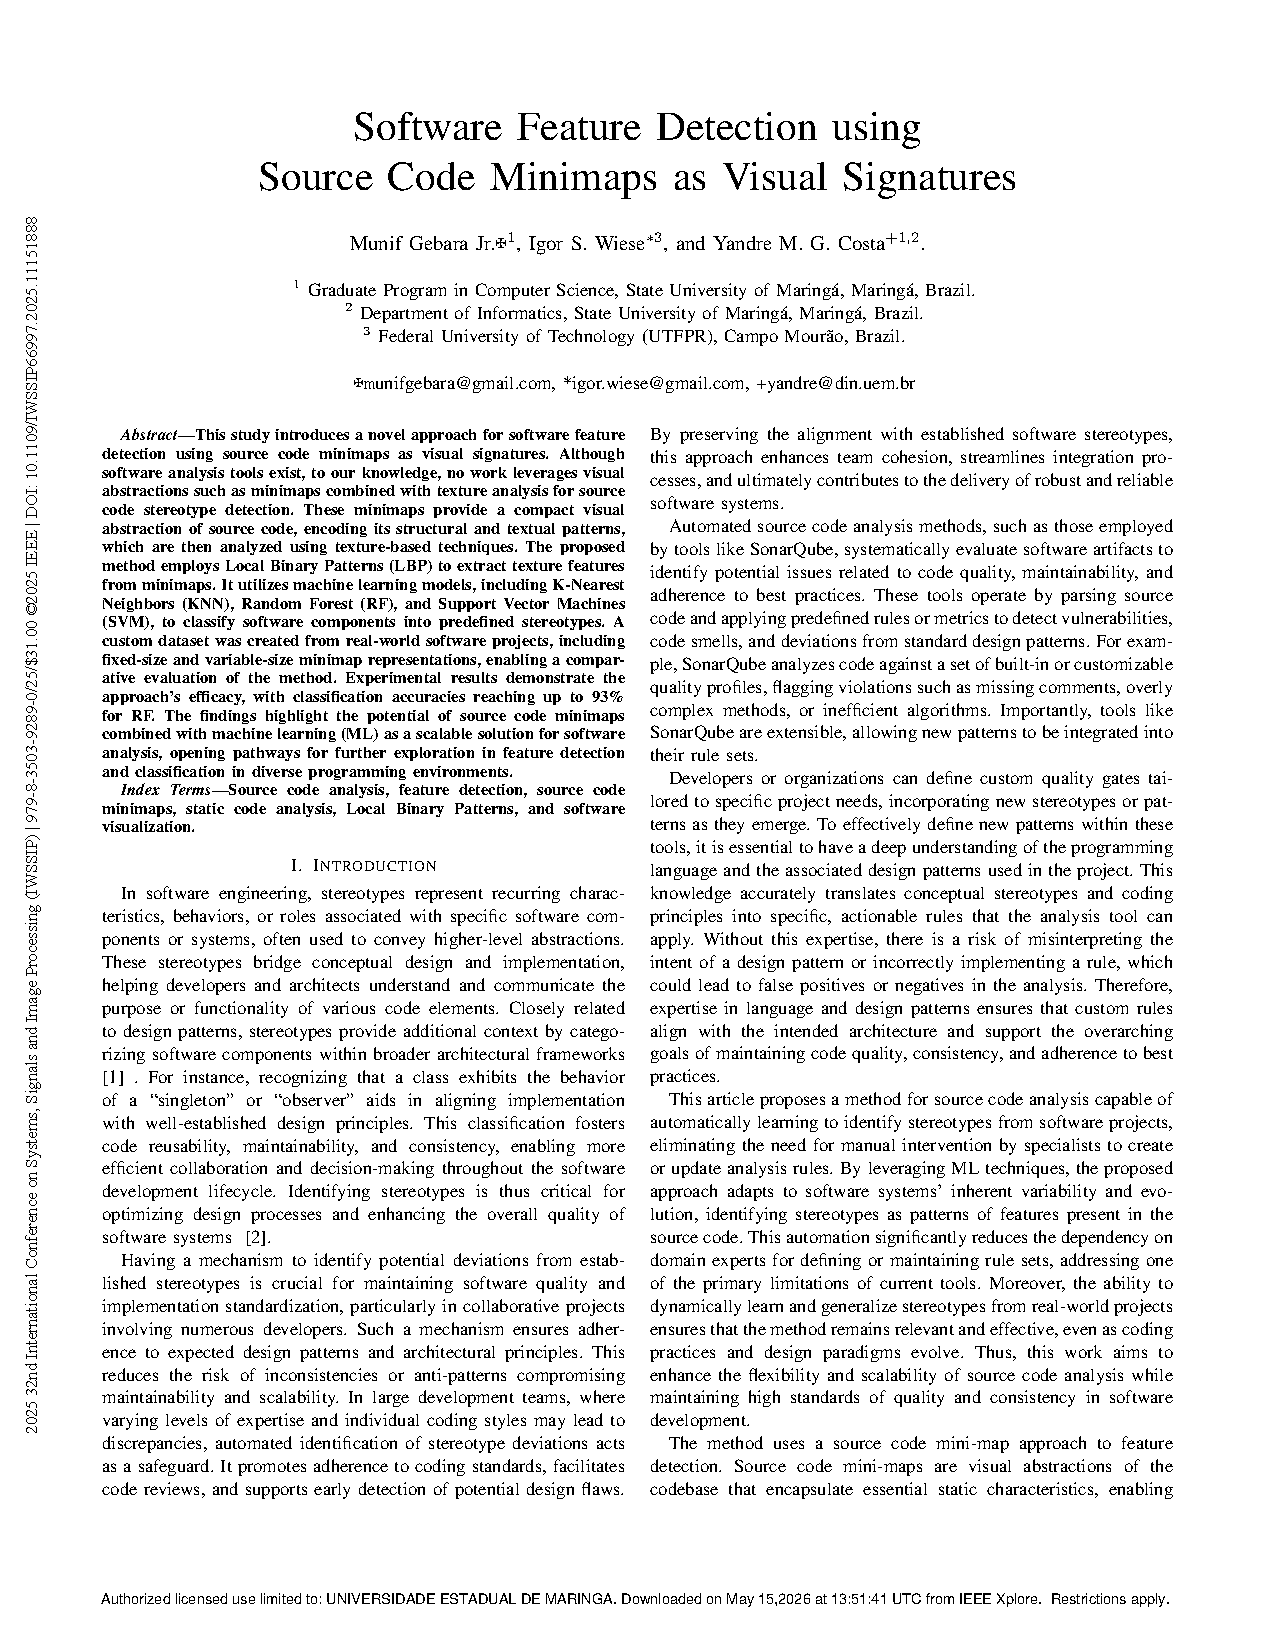
\includepdf[pages=-]{apendices/apendice-a-iwssip2025.pdf}

\chapter{Article published at CIARP 2025: Source Code Minimaps at Scale: Feature-Oriented Analysis of 100 Projects}
\label{apendice:ciarp}
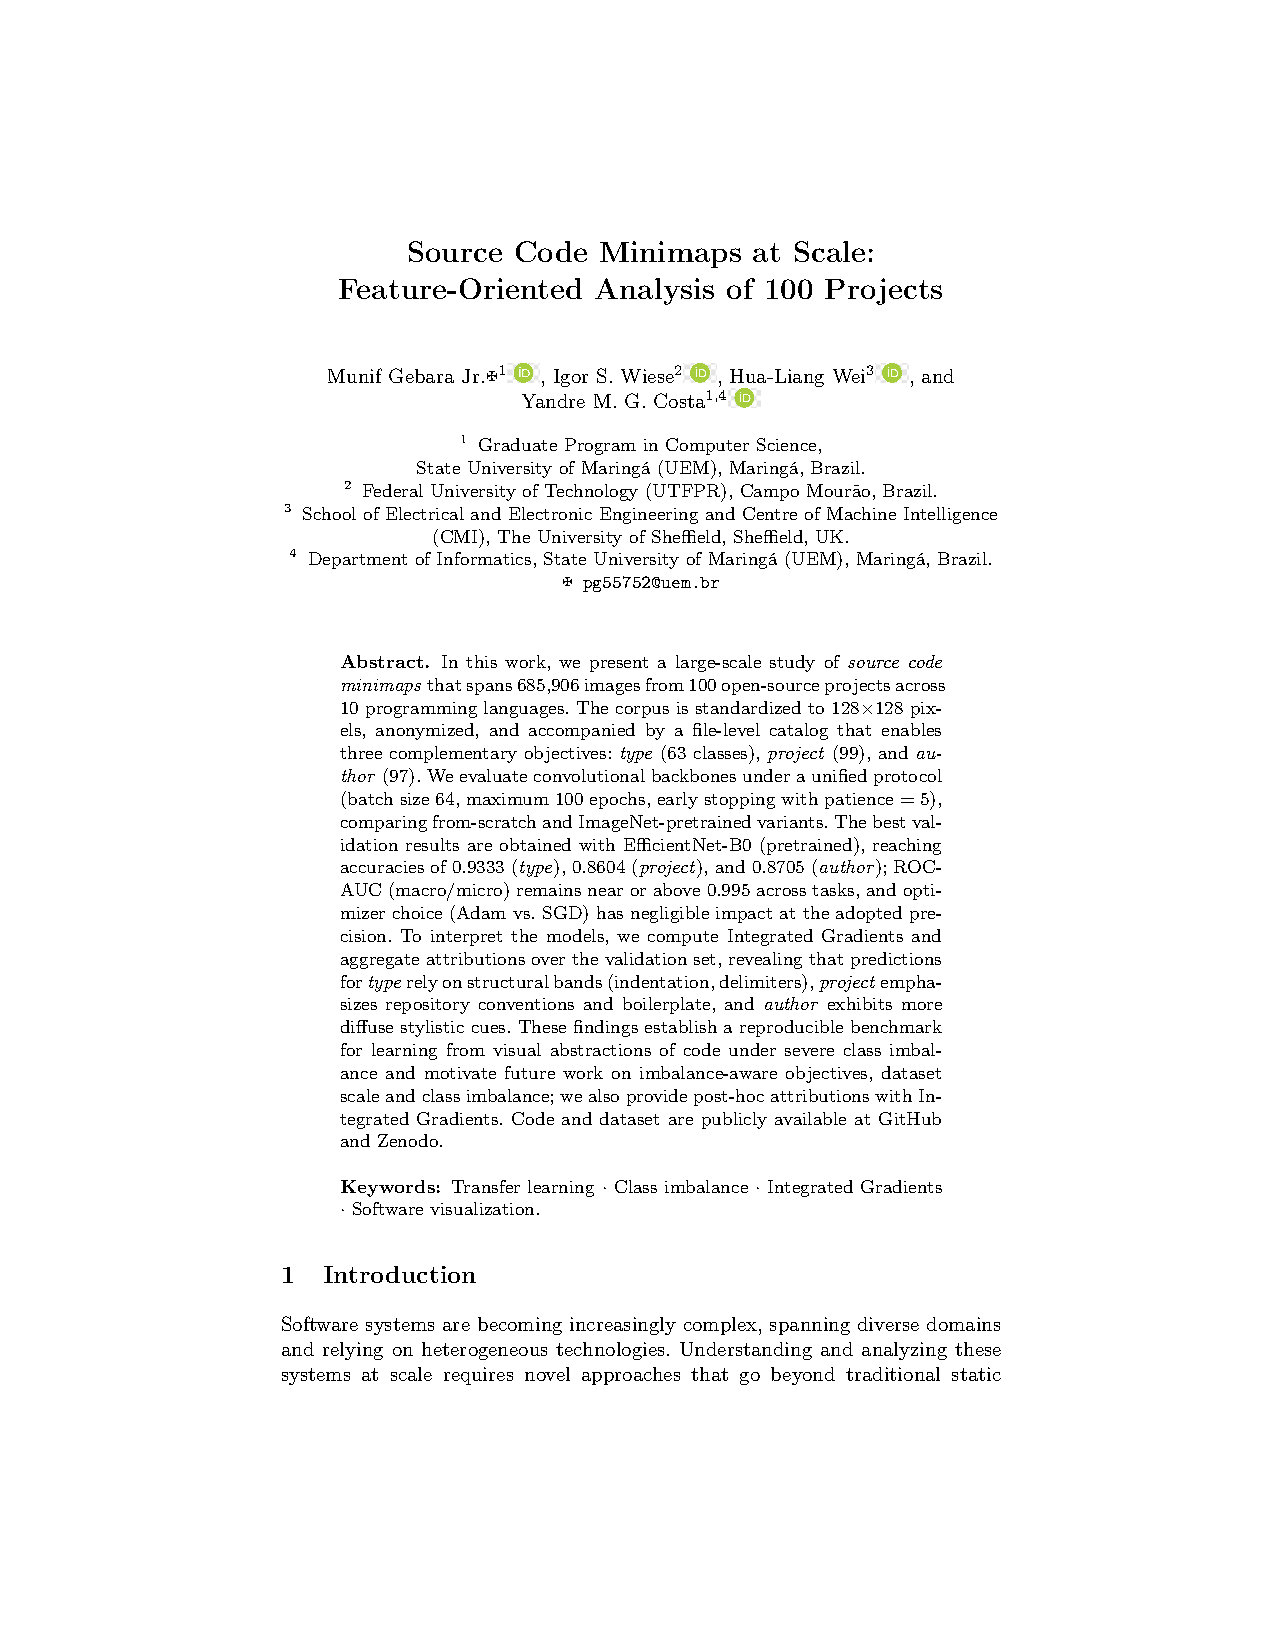
\includepdf[pages=-]{apendices/apendice-b-ciarp2025.pdf}

\chapter{Article accepted at SBES-Tools 2026: MinimapSignatures: A Multi-IDE Ecosystem for Analysis of Visual Source Code Signatures}
\label{apendice:sbes}
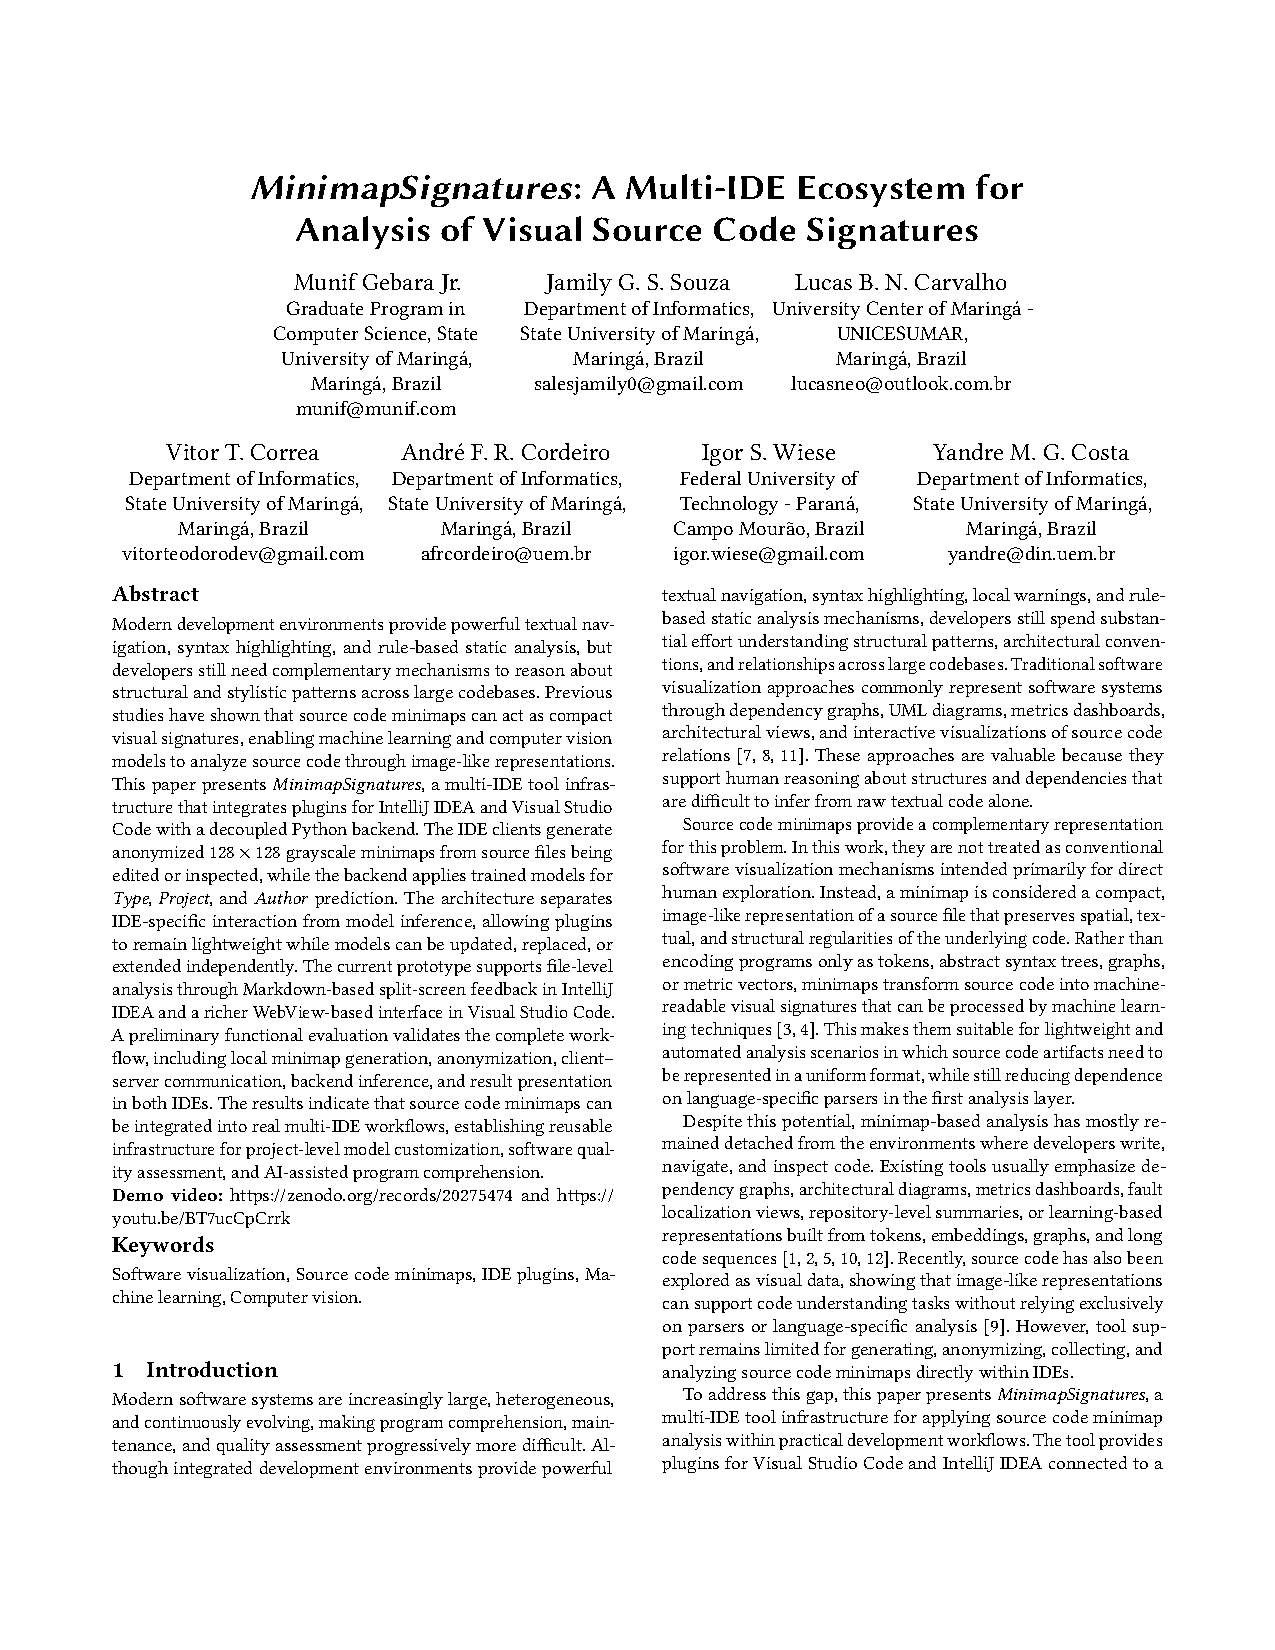
\includepdf[pages=-]{apendices/apendice-c-sbes2026.pdf}

\end{apendicesenv}

% ------------------------------------------------------------------------
% Annexes: third-party documents (ABNT: material not produced by the author)
% ------------------------------------------------------------------------
\begin{anexosenv}
\partanexos

\chapter{CAPES award letter for the doctoral research internship abroad (PDSE)}
\label{anexo:pdse}
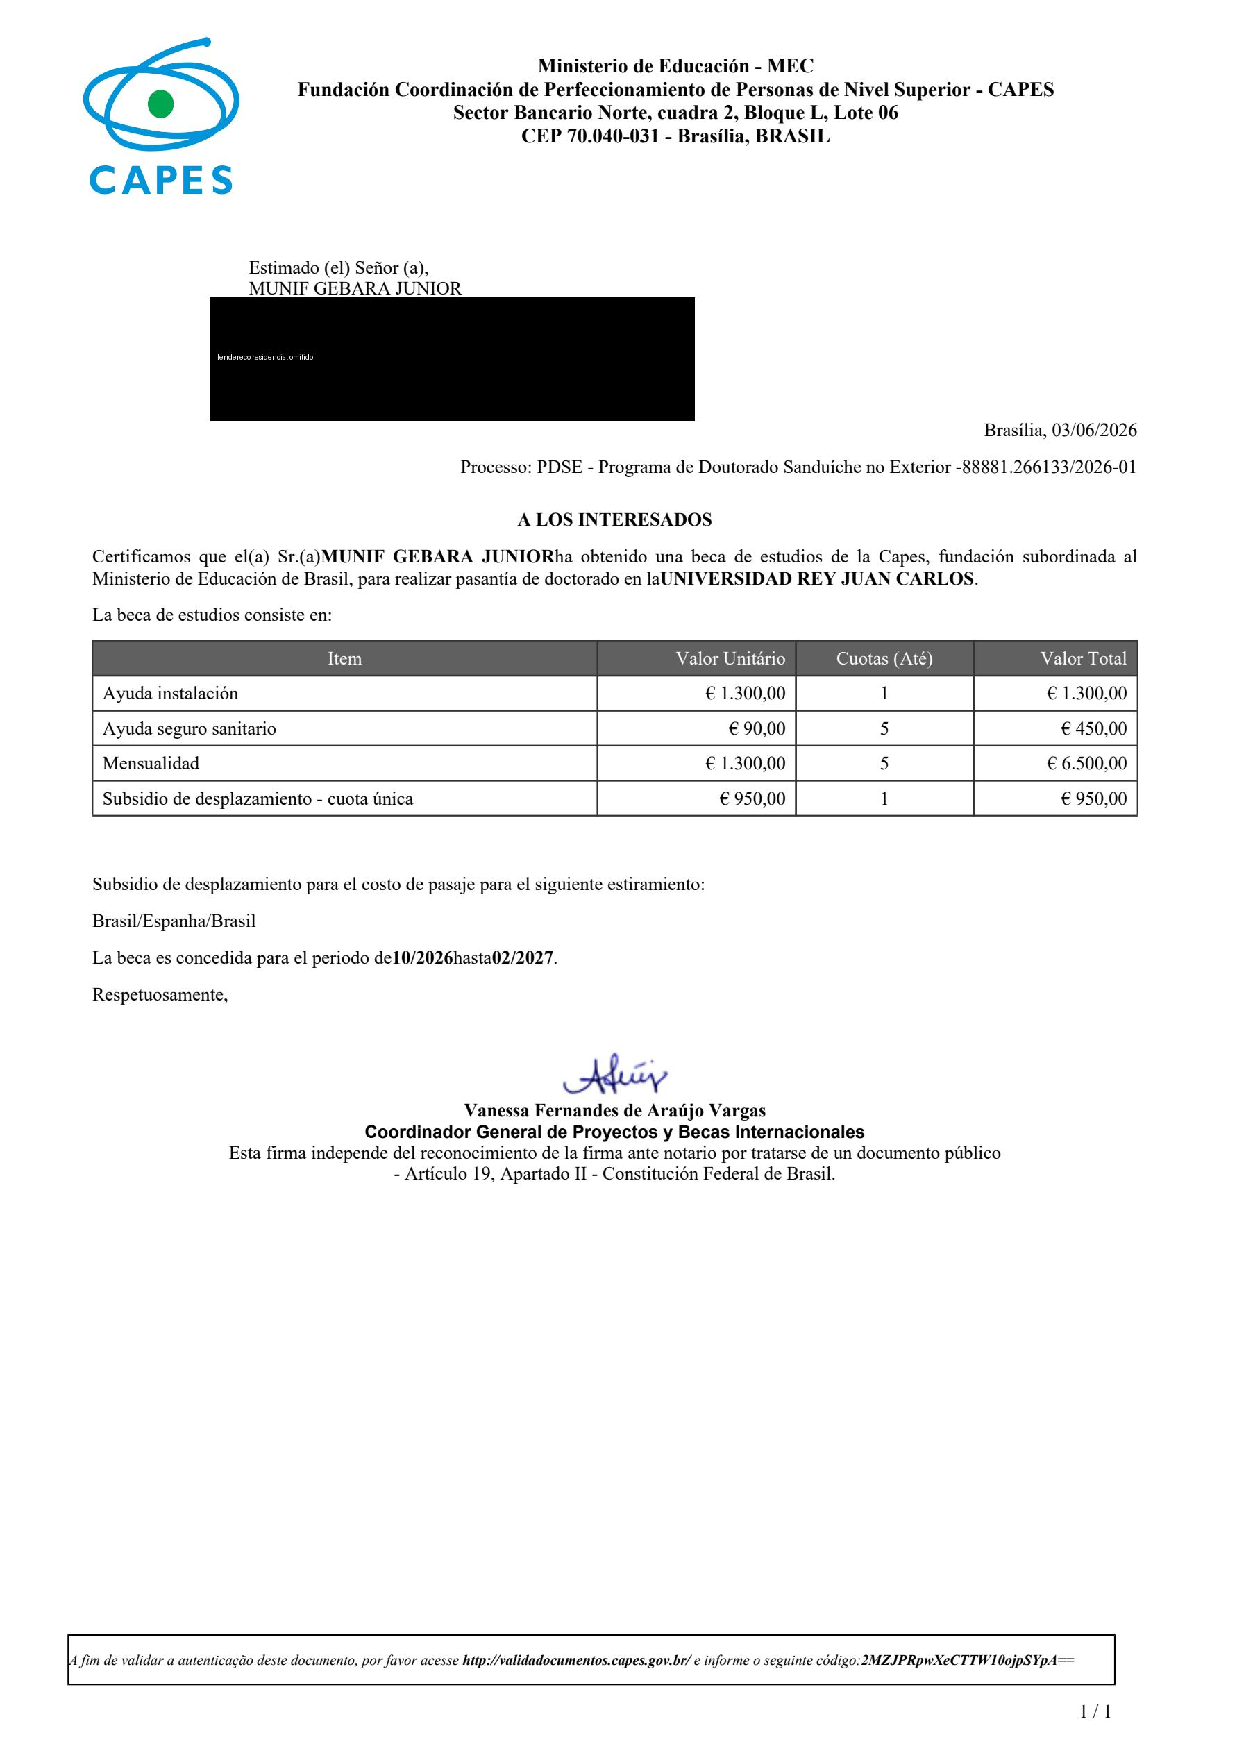
\includepdf[pages=-]{anexos/anexo-a-carta-pdse.pdf}

\end{anexosenv}

\end{document}
